\setcounter{footnote}{0}
\setcounter{section}{0}
\setcounter{ExNo}{0}
\begin{center}
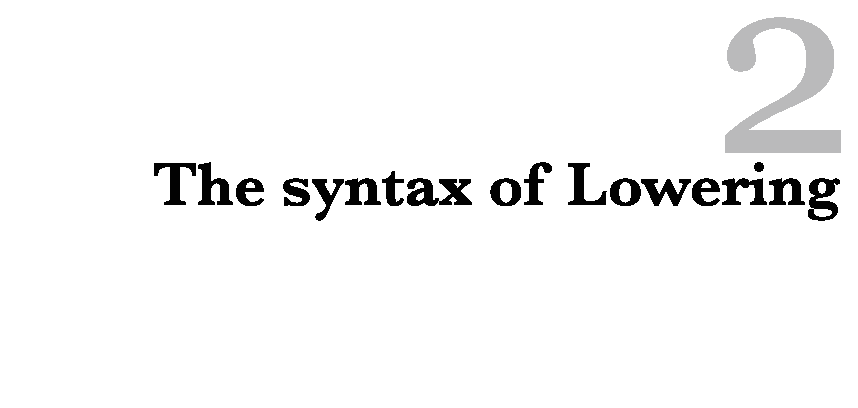
\includegraphics{chapter2.eps}
\end{center}
\section*{}
\addcontentsline{toc}{section}{\Large{Chapter 2: The syntax of Lowering}}
\section{Overview}
In this chapter, I investigate some of the structural properties of Lowering, focusing on the operation of Lowering as a head movement transformation that is inherently sensitive to hierarchical syntactic composition. Lowering, just like Raising of heads in the narrow syntax, is limited by strict locality conditions; just as narrow syntactic head movement is restricted to movement of a head to the next highest head, skipping specifiers and adjuncts (the \textit{Head Movement Constraint} (HMC), \citenop{travis1984}), Lowering of a head X must target the head Y of its complement, thus also necessarily skipping any intervening specifiers and adjuncts. Therefore, in many respects, Lowering of heads at PF is simply the structural inverse of Raising of heads in the narrow syntax. The current chapter attempts to account for the similarities and differences between these two types of structural head movement in a principled manner.

Recall from Chapter 1 that all downward movements are prohibited in the narrow syntax, by assumption, and thus Lowering must occur on the PF branch after Spell-out.\footnote{As noted in Chapter 1, I will initially follow \posscitet{embick_noyer2001} model of Lowering as a PF operation, though we will revise this view in later chapters.} Additionally, Lowering, as it must necessarily be operative on syntactic structures, since it specifically targets syntactic heads and is immune to any blocking effects of intervening specifiers or adjuncts, occurs before Vocabulary Insertion (i.e.\ before the formation of a morpho-phonological string). Lowering is thus defined and represented schematically as follows (adapted from \citeauthor{embick_noyer2001} \citeyear{embick_noyer2001}:561):\footnote{Note that the directionality of adjunction of X to Y is, for the most part, unimportant. We will address the resulting orderings of these morphemes in the morpho-phonological string in the upcoming sections.}

\singlespacing
\begin{quote}
\begin{minipage}{5in}
\ex. \textit{Lowering (to be revised)} \label{Lowering_def}
\a. A head X$^{0}$ may be lowered to the head of its complement Y$^{0}$ after Spell-out, but before Vocabulary Insertion.\\
\b.[][$_{XP}$ X$^{0}$ ... [$_{YP}$ ... Y$^{0}$ ... ]] $\rightarrow$ [$_{XP}$ ... [$_{YP}$ ... [$_{Y}$\raisebox{-3pt}{$^{\circ}$} Y$^{0}$ + X$^{0}$] ... ]]\\
\b. \Tree
[.XP ZP
[.XP \node{Xtrace}t 
[.YP WP
[.YP [.Y\0 \node{X}{~~X\0~~} ~~Y~~ ] $\ldots$
].YP ].YP ].XP ]
\anodecurve[bl]{Xtrace}[bl]{X}{1in}\\\\

\end{minipage}
\end{quote}
\onehalfspacing
In the remainder of this section, we will see many purported examples of the above operation, and begin to develop certain analytical criteria that will allow us to identify Lowering transformations. While most of this and the next chapter will focus on Lowering (and Local Dislocation) operations within verbal paradigms cross-linguistically (e.g.\ tense-hopping, Lowering of Aspect to the verb), we will also address the possibility of such transformations within the nominal domain (e.g.\ Lowering of determiners within the DP, as in Bulgarian).

In Section 2 of this chapter, using examples of reduplication in Tagalog and Ndebele and subject agreement markers in Turkish, I argue that Lowering operations can be much more varied than narrow syntactic head movement, due simply to the opposite directionality of each respective movement and the correlating higher level of available complexity of the landing site for Lowering heads than for Raising heads. In other words, unlike in narrow syntactic head movement, the head that is the targeted landing site for a Lowering operation may be structurally complex, as the result of previous narrow syntactic head movements, thus allowing for the possibility of multiple adjunction sites when Lowering into a complex head. I propose that this derives several cases of morphological optionality, in which the position of a particular morpheme within a word may vary considerably with respect to the positions of other morphemes in the overt representation of that word.

In Section 3, we investigate the motivations underlying Lowering operations, which have heretofore been elusive. Taking the relatively uncontroversial stance that 1) all transformations of syntactic structure (including head-to-head Lowering) should be feature-driven, and 2) structural transformations in the narrow syntax are preferred to---i.e.\ are more economical than---structural transformations after Spell-out (due, for example, to the Earliness Principle \citep{pesetsky1989}), I propose an extension to the \textit{Phase Impenetrability Condition} (PIC, \citenop{chomsky2001}) that accounts for these seemingly uneconomical downward head movements at PF. Namely, I argue for the \textit{Phase Head Impenetrability Condition} (PHIC), under which embedded features of a complex phase head become unavailable for subsequent narrow syntactic feature-checking after phase Spell-out. Lowering is therefore evaluated when the PHIC disallows an uninterpretable feature on a higher head to be checked via narrow syntactic (i.e.\ upward) head movement; that is, the required interpretable feature embedded in the phase head is unable to be accessed by the corresponding uninterpretable feature on the higher head, due to the PHIC. This accounts for the general observation that Lowering only ever seems to occur between a head that takes a phase complement and the head of that phase (e.g.\ T-to-\textit{v}, Asp-to-\textit{v}, and D-to-\textit{n} Lowering, among others). Section 4 summarizes the preceding arguments and presents a few remaining issues with the proposed model, many of which are to be addressed in later chapters.\footnote{The reader should keep in mind that I will be ignoring the motivations underlying the transformations in \S1 and \S2 until \S3, and instead will be addressing these patterns from a purely structural perspective. However, note that I will later argue that each Lowering head that we observe carries an uninterpretable feature that it may not check via raising of the lower head, due to the PHIC, and so the higher head must therefore move downward to the lower head.}

\subsection{Tense-hopping}
In this section, we will briefly examine one of the most well-known examples of Lowering: affix-hopping of finite tense in verbal paradigms (\citenop{chomsky1957}, \citenop{embick_noyer2001}, and many others). As we saw in Chapter 1, some languages, such as French, raise the verb out of \textit{v}P to the T head, whereas others, such as English and Swedish, leave the verb within \textit{v}P (in embedded clauses in the case of Swedish), yet the morphology of the higher T head is realized overtly on the lower verb. As downward movements are assumed to be impossible in the narrow syntax, the overt morphological realizations of these inflected tense-hopping verb forms require explanation.

\subsubsection{A brief note on competing theories of tense-hopping}
Providing an account of the patterns of tense-hopping has been, to varying degrees, at least one of the goals of most models of (morpho-)syntactic theory ever since \citet{chomsky1957}.\footnote{Or, at the very least, a theory of tense-hopping has been provided as a bit of ``house-keeping'' in most theories of syntactic derivation.}  Because of this, it would be impossible to provide a fair treatment of all of these various accounts, and so I will not attempt to do so here. I will simply note briefly that there are two general schools of thought on the subject, as mentioned in Chapter 1: the lexicalist view and the non-lexicalist view. Under the lexicalist view (e.g.\ \citenop{chomsky1993}), verbs come into the narrow syntactic derivation fully inflected, and all verbs raise to INFL to check their inflectional features. The difference between verb-raising languages and tense-hopping languages under this analysis is that the former raise these verbs before PF (i.e.\ INFL has strong features), whereas the latter raise these verbs at LF (i.e.\ INFL has weak features). Distributed Morphology (DM, \citenop{halle_marantz1993}), on the other hand, takes a decidedly non-lexicalist approach to these patterns. Under DM, all verbs enter the syntax uninflected, as there is no pre-syntactic generative lexicon, and so all complex inflected verb forms must be created via syntactic and/or post-syntactic transformations of discrete morphemes.

Neither of these theories is without both its advantages and its drawbacks. For example, the lexicalist view renders downward transformations a completely unnecessary complication to syntactic derivation, but, unlike the non-lexicalist approach, this requires the existence of an additional pre-syntactic generative component of linguistic computation, the capabilities and limitations of which are difficult to pin down. Moreover, auxiliary-raising in English creates problems for the standard accounts of tense-hopping under both models; e.g., under the lexicalist view, auxiliaries may not wait until LF to raise, for uncertain reasons,\footnote{\citet{chomsky1993} argues that this is because auxiliaries are semantically vacuous, and so therefore cannot be targeted by movement at LF. However, since overt movement is necessarily evaluated before covert movement, this scenario would seem to require an undesirable pre-PF-Spell-out look-ahead to the possibility or impossibility of later movement at LF, under a purely derivational model of syntax.}  and under the non-lexicalist view, tense-hopping is somehow made unnecessary in favor of verb-raising in the presence of an auxiliary.\footnote{\citet{lasnik1995} proposes a hybrid lexicalist/non-lexicalist approach for English verbs in which auxiliaries, but not main verbs, come into the derivation fully inflected. We will address this in Chapter 4 and present an alternative, purely non-lexicalist approach for both.}  However, it is not a goal of this thesis to argue extensively for one theory over the other (but see the brief discussion in Chapter 1 \S2.1), but rather to adopt one of these theories, namely Distributed Morphology, and account for the patterns of tense-hopping and other morphological phenomena using the mechanisms made available by that model of complex word formation. Therefore, I will leave the discussion of competing morphological theories here and move on to an analysis of tense-hopping under DM.

\subsubsection{Tense-hopping under DM}
We will begin with a brief overview tense-hopping from the perspective of Distributed Morphology, under which the pattern is derived via Lowering. Consider the following example from Swedish:\footnote{Note that Swedish is V2 in matrix, but not embedded, clauses. We will address this issue in Chapter 3, in which I provide a cross-linguistic comparison of Swedish and English tense-hopping. Note that I will not address English tense-hopping in this chapter, as I ultimately claim that it is not a case of Lowering, following the general claims of \citet{bobaljik1995}, \citet{lasnik1995}, \citet{ochi1999}, and \citet{omaki2008}. However, we will maintain the Lowering analysis of Swedish tense-hopping throughout this thesis.}

\singlespacing
\begin{quote}
\begin{minipage}{5.5in}
\ex. \label{Se_completely}
\ag. Du vet att jag \textbf{helt} \underline{gl\"{o}mde} adressen.\\
you know.\sc{past} that I completely forget.\sc{past} address.\sc{def}\\
`You know that I completely forgot the address.'\\
\bg. *Du vet att jag \underline{gl\"{o}mde} \textbf{helt} adressen.\\
you know.\sc{pres} that I forget.\sc{past} completely address.\sc{def}\\

\end{minipage}\\\\
\end{quote}
\onehalfspacing
In the embedded clause in (\ref{Se_completely}), the \textit{v}P-adjunct \textit{helt} `completely' appears before the embedded verb \textit{gl\"{o}mde} `forgot', indicating that the verb has not raised out of the \textit{v}P. This suggests a syntactic structure at Spell-out like the following (\textit{gl\"{o}mma} is the infinitival, uninflected form of `forget'):

\singlespacing
\begin{quote}
\begin{minipage}{5in}
\ex. \textit{Du vet att jag helt gl\"{o}mde adressen.} \label{Se_completely_tree}

\moveleft12pt\vbox{\small{~~~~~~~~~~~~~... \Tree
[.TP \qroof{\{\textit{jag}\}}.DP_i
[.TP T\\\{\sc{past}\}
[.\textit{v}P \qroof{\{\textit{helt}\}}.AP
[.\textit{v}P \textit{t}_i
[.\textit{v}P [.\textit{v} V_j\\\{\textit{gl\"{o}mma}\} \textit{v} ]
[.VP t_j \qroof{\{\textit{adressen}\}}.DP
].VP ].\textit{v}P ].\textit{v}P ].\textit{v}P ].TP ]\\}}
\end{minipage}
\end{quote}
\onehalfspacing
Given that the verb has not moved out of \textit{v}P, yet the higher inflectional past tense morpheme appears on the overt form of the verb, T in (\ref{Se_completely_tree}) must undergo a downward movement on the PF branch. According to \citet{embick_noyer2001}, tense-hopping, like that observed in the Swedish example above, is the result of T-to-\textit{v} Lowering. Under this analysis, the morpheme in T in (\ref{Se_completely_tree}) undergoes Lowering to the head of its complement after Spell-out but before Vocabulary Insertion. Since this is a case of head-to-head movement, the phrase adjoined to \textit{v}P, {\it helt}, is necessarily skipped in this structural transformation, whether it is merged early or late (see Chapter 1 \S3.1, and Chapters 3 and 4).

\subsubsection{\posscitet{cinque1999} Functional Cartography}\label{cinque_sec}
Before we may accept such an analysis of supposed tense-hopping transformations like the one observed in the Swedish example above, we must ask whether it is actually the case that the morpheme in T has lowered to the verb, or if the verb itself has rather raised to finite T, and the adverb is simply higher than T (with the subject in some even higher position). \citet{cinque1999} observed that there is a universal relative ordering of adverbs in the functional domain of clauses. For example, adverbs like \textit{probably} must always appear structurally higher than adverbs like \textit{completely}:\footnote{In the absence of any focus or intonational pauses, (\ref{En_prob_compl}b) can only be understood as \textit{completely} directly modifying \textit{probably}, showing that it may not take scope over the remainder of the clause. Consequently, [\textit{completely probably}] itself must form its own, single syntactic constituent, with \textit{completely} adjoined to \textit{probably}.}

\begin{quote}
\ex. \label{En_prob_compl}
\a. John probably completely lost his mind.
\b. ?* John completely probably lost his mind.

\ex. \label{Fr_prob_compl} \textit{French}
\ag. Il a probablement compl\`{e}tement perdu la t\^{e}te.\\
he has probably completely lost the head\\
`He probably completely lost his mind'\\
\b. ?* Il a compl\`{e}tement probablement perdu la t\^{e}te.

\end{quote}
Taking this and many other universal, rigid ordering patterns into consideration, Cinque proposes that there is a strictly ordered cartography of functional heads (i.e.\ heads found above the lexical, verbal domain (see \S2.1.1 below and Chapter 3)), which is a part of Universal Grammar. These heads project the adverbs in question in their specifiers, and thus these adverbs are universally ordered across languages. In this way, Cinque argues that all languages contain a great number of functional heads, and the order in which these are projected in the syntax is universally fixed. For example, here is one version of this hierarchy:

\begin{quote}
\begin{minipage}{4.5in}
\ex. \label{Cinque_hierarchy} \textit{Cinque's functional hierarchy}\\
MoodP$_{speech}$ $_{act}$ $\gg$ MoodP$_{evaluative}$ $\gg$ MoodP$_{evidential}$ $\gg$ ModP$_{epistemic}$ $\gg$ TP$_{(Past)}$ $\gg$ TP$_{(Future)}$ $\gg$ MoodP$_{irrealis}$ $\gg$ ModP$_{alethic}$ $\gg$ AspP$_{habitual}$ $\gg$ AspP$_{repetitive(I)}$ $\gg$ AspP$_{frequentative(I)}$ $\gg$ ModP$_{volitional}$ $\gg$ AspP$_{celerative(I)}$ $\gg$ TP$_{(Anterior)}$ $\gg$ AspP$_{terminative}$ $\gg$ AspP$_{continuative}$ $\gg$ AspP$_{retrospective}$ $\gg$ AspP$_{proximative}$ $\gg$ AspP$_{durative}$ $\gg$ AspP$_{generic/progressive}$ $\gg$ AspP$_{prospective}$ $\gg$ ModP$_{obligation}$ $\gg$ ModP$_{permission/ability}$ $\gg$ AspP$_{Completive}$ $\gg$ VoiceP $\gg$ AspP$_{celerative(II)}$ $\gg$ AspP$_{repetitive(II)}$ $\gg$ AspP$_{frequentative(II)}$\\ 

\end{minipage}
\end{quote}
According to this hierarchy, the reason that \textit{probably} is universally higher than \textit{completely} is because \textit{probably} is generated in SpecModP$_{epistemic}$,\footnote{Cinque notes that adverbs like \textit{probably} suggest the same lack of confidence on the part of the speaker as epistemic modals like \textit{should} do when expressing doubt; e.g.\ \textit{John should be home now (�but I'm not sure if he is)}. Thus, \textit{probably} is functionally related to these modals by virtue of being generated in the specifier position of the head that contains them, under his analysis.}  whereas \textit{completely} is generated in the structurally lower SpecAspP$_{completive}$. Assuming that this hierarchy of functional heads is correct, it gives us cause to question whether adverbs like the one in the Swedish example in (\ref{Se_completely}) are simply generated in the specifier of one of the higher functional heads of this cartography, and the verb raises in the narrow syntax to a tense morpheme found in one of the lower functional heads (i.e.\ there is actually no tense-hopping involved in this pattern). Even a cursory examination of the above hierarchy suggests that this is not a possibility. Within this hierarchy, the adverb \textit{helt} `completely' should be generated relatively low (e.g.\ in SpecAspP$_{completive}$), but the past tense morpheme should be generated relatively high (e.g.\ in TP$_{(past)}$). Therefore, given that the inflected verb in (\ref{Se_completely}) follows the adverb \textit{helt}, the verb could not have possibly raised higher than the head of AspP$_{completive}$, which is still lower than the base-generated position of finite past tense. This requires that, even if we accept the consistent presence of these functional heads in the narrow syntactic structure, the tense morpheme must still undergo some type of downward transformation to adjoin to the verb before the ultimate PF representation is derived, given our rejection of a lexicalist model of verbal inflection (see Chapter 1 and \S1.1.1 above).

Additionally, under a non-lexicalist morphology that allows for head-to-head Lowering, such an ever-present, expanded functional cartography can almost certainly not exist. Since Lowering is limited to a strict head-complement locality, this type of fine functional domain places overly restrictive conditions on what types of Lowering are possible. For example, it would limit Lowering to Mod$_{epistemic}$-to-T$_{(Past)}$, Asp$_{terminative}$-to-Asp$_{continuative}$, etc., and would not allow for the putative cases of T-to-{\it v} Lowering, as these two morphemes would not be in a head-complement relation. We would instead have to re-think what locality conditions are operative in Lowering transformations, and undoubtedly allow for iterative head-lowering, for which I have found no empirical evidence.

Taking into account the fact that such a cartographic approach to adverb placement does not obviate the need for some type of tense-hopping transformation, and creates problems for the notion of locality in morpho-syntactic transformations, I will not adopt Cinque's hierarchy of functional heads for the remainder of this thesis, and will rather assume that the incontrovertible ordering patterns that he observed are the result of some as yet undetermined syntactic or semantic restrictions on the order and placement of adjuncts to pre-existing phrasal projections (see \citenop{ernst2006}, \citenop{nilsen2003} for relevant proposals). The assumption here will therefore be that the strict ordering of adverbs is not due to the presence of a fixed cartography of functional heads, but it is rather due to a restriction on either the order in which these adjuncts may be merged into the narrow syntactic structure or, relatedly, some type of scope restrictions at LF. It is beyond the range of the current project to propose, or even conjecture about, what these restrictions might be. I will simply assume that (at least most) verbal modifiers are adjuncts to a \textit{v}P projection, as schematized in (\ref{Se_completely_tree}), rather than specifiers of independent functional heads. Therefore, whether an inflected verb appears immediately before or after these \textit{v}P-adjuncts will allow us to determine if a particular construction is the result of verb-raising or tense-hopping, respectively.\footnotemark \footnotetext{This of course does not hold in the case of right-adjoined modifiers like the following, which necessarily follow both the verb and its complement, just as in English, and thus do not allow us to make any strong claims about the relative positions of tense and the verb:

\singlespacing
\begin{quote}
\ag.[(i)] Du vet att jag l\"{a}ser tidningen ofta.\\
you know.\sc{pres} that I read.\sc{pres} newspaper.\sc{def} often\\
`You know that I read the newspaper often.'

\end{quote}
However, just as in English, this modifier may also be left-adjoined, which is the configuration that we are most concerned with here:

\singlespacing
\begin{quote}
\ag.[(ii)]Du vet att jag ofta l\"{a}ser tidningen.\\
you know.\sc{pres} that I often read.\sc{pres} newspaper.\sc{def}\\
`You know that I often read the newspaper.'

\end{quote}
I should take this opportunity to note that I am not adopting a syntactic linearization model like \posscitet{kayne1994} \textit{Antisymmetry}. I instead entertain the possibility that there are both left- and right-adjunction, in addition to both left- and right-headedness (e.g.\ Turkish, \S2.3).}$^{,}$\footnote{I will also not entertain the non-standard assumption that all apparently intervening adjuncts are actually always adjoined to TP, rather than \textit{v}P (see \citenop{boskovic_lasnik2003}). Among other things, this complicates an analysis of modals, which I assume to be located in T, with respect to adverbs, e.g.\ \textit{Bill would often eat pie}, in which the modifier is necessarily adjoined to a position below T and above the verb, under the current analysis.} In this way, we allow for a much simpler syntactic derivation, with as few projections as possible, which will be an underlying goal of many of the proposals presented in this work.\footnote{\begin{samepage}This assumption is unproblematic for English and Swedish, which are our main concern here, as they are argued to have a `pre-Pollockian' unsplit-INFL (\citenop{bobaljik1995}, \citenop{thrainsson1996}, \citenop{bobaljik_thrainsson1998}). That is, unlike languages with multiple Agr projections in the domain of INFL, English and Swedish simply have the following structure:\nobreak
\begin{quote}
\a.[(i)] \Tree
[.TP Spec [.TP T \qroof{$\ldots$}.\textit{v}P ].TP ]

\end{quote}
In split-INFL languages, such as Italian and French, there are theoretically more possible adjunction sites. See Chapter 3, \S2.3 for more.\end{samepage}} I will close the discussion of tense-hopping here, but will take it up again in much more detail in Chapter 3.

\subsection{Determiner-hopping}
Lowering is argued to not be limited to tense-hopping constructions. For example, determiners in many languages undergo a downward transformation to adjoin to the noun head, which is ostensibly the result of a Lowering operation. Consider the following Bulgarian data (from \citenop{embick_noyer2001}) in which the definiteness marker appears adjoined to the noun head in (\ref{Bg_data}a) and the adjective in (\ref{Bg_data}b), but may not adjoin to the adverb in (\ref{Bg_data}c):

\singlespacing
\begin{quote}
\begin{minipage}{5in}
\ex. \label{Bg_data}
\ag. kniga-ta\\
book-\sc{def}\\
\hspace{1pt}\\
\bg. xubaba-ta kniga\\
nice-\sc{def} book\\
\hspace{1pt}\\
\cg. *mnog-\textschwa t star teat\textschwa r\\
very-\sc{def} old theater\\
\hspace{1pt}\\
\dg. mnogo \mbox{starij-\textschwa} teat\textschwa r\\
very old-\sc{def} theater\\
\hspace{1pt}\\

\end{minipage}
\end{quote}
\onehalfspacing
Assuming, following \citet{abney1987}, that the adjective AP is generated on the spine of the DP, and that the definiteness marker is the head of the DP, the pre-Spell-out structure for (\ref{Bg_data}d) is the following, in which the adverb \textit{mnogo} `very' is an adjunct:\footnote{I assume that whether AP is generated on the spine or as an adjunct is parameterized cross-linguistically. In Chapter 4, I will show that the same type of parameterization occurs with negation.}

\singlespacing
\begin{quote}
\ex. \label{Bg_tree}
\Tree
[.DP D\\\{\sc{def}\}
[.AP \qroof{\{\textit{mnogo}\}}.AdvP
[.AP A\\\{\textit{star}\} [ N\\\{\textit{teat\textschwa r}\} ].NP
].AP ].AP ] 

\end{quote}
\onehalfspacing
Embick and Noyer argue that in (\ref{Bg_tree}) post-Spell-out Lowering moves the head D to the head of its complement, A, skipping the intervening adjunct.\footnote{In \S4 below, I argue that an analysis of Bulgarian determiner-hopping as Lowering due to the PHIC is problematic. However, in Chapter 4 we will re-analyze this data as a possible case of Local Dislocation.}  In the absence of the AP projection (and, less importantly, the AdvP adjunct), D will take NP as its complement, and thus D lowers directly to N, as in (\ref{Bg_data}a). However, in the presence of this AP, D may not lower all the way to N (\ref{Bg_data}b,d), but must necessarily target just the head of its complement, A. Thus, movement of the determiner in Bulgarian is argued to be a post-Spell-out head-to-head transformation---i.e.\ Lowering--, and Lowering is limited to the simple, one time operation of moving a head to the head of its complement; that is, there is no evidence that Lowering may be iterative downward head movement (e.g.\ D may not move iteratively through A to N in Bulgarian). Note that this is unlike narrow syntactic head movement, which is argued to allow iteration in keeping with the HMC; we will address why this distinction exists in the following sections and in Chapter 3.

\subsection{Section summary}
In this section we have seen that Lowering is a strictly local, downward head-to-head movement operation occurring after Spell-out to the PF branch. It may not be iterative, nor may it skip intervening head projections, though adjoined phrases are transparent for this movement. However, the motivations behind these transformations remain unclear. We must ask the following questions: what drives Lowering, and why can't this requirement be met via narrow syntactic raising? We will address this issue in Section 3, but will first investigate the intricate structural sensitivity that is possible in Lowering operations.

\section{Structural sensitivity of Lowering operations: Morphological optionality}
In some languages, certain reduplicative operations may produce several distinct overt realizations, all of which are used in free variation by native speakers, and carry no semantically intelligible differences. One such example is Tagalog aspectual reduplication, where the position of the reduplicant may fluctuate within the verb. In the following cases, reduplication in Tagalog indicates that the entire event is unrealized----i.e., roughly, it is not yet complete (from \citenop{rackowski1999}; \textbf{boldface} and brackets `[]' indicate the reduplicative aspectual morpheme):

\singlespacing
\begin{quote}
\begin{minipage}{5in}
\ex. \label{Ta_tm_red_ex}
\a. \textit{Base form}
\bg.[] ma- \textglotstop i- pa- bili\\
\mbox{\sc{abl}}- \mbox{\sc{tm}}- \mbox{\sc{caus}}- buy\\
`be able to have (s.o.) buy'\\
\b. \textit{Reduplicated outputs}
\c.[] ma-\textglotstop i-pa-[\textbf{bii}]-bili
\d.[] ma-\textglotstop i-[\textbf{paa}]-pa-bili
\e.[] `will be able to have (s.o.) buy'\\

\end{minipage}
\end{quote}
\onehalfspacing
In (\ref{Ta_tm_red_ex}), either the verb root \textit{bili} or the causative morpheme \textit{pa-} may be targeted for reduplication.\footnote{See \S2.1 for the status of the ability marker \textit{ma-} and the topic marker \textit{\textglotstop i-} in reduplication.}

A similar example is the case of reduplication in the Bantu language Ndebele. Here, a phonologically small root allows for the optional copying of affixes into the reduplicant (data from \citenop{sibanda2004}):\\

\singlespacing
\begin{quote}
\ex. \label{Nd_red_shortex}
\a. \textit{Base form}
\bg.[] zw -is -a\\
taste	-\sc{caus} -a\\
`cause to taste'\\
\b. \textit{Reduplicated outputs}
\c.[] [\textbf{zwisa}]-zw-is-a
\d.[] [\textbf{zwayi}]-zw-is-a
\e.[] `cause to taste a bit'\\

\end{quote}
\onehalfspacing
In (\ref{Nd_red_shortex}), the causative suffix -\textit{is} may be optionally copied into the reduplicant; when it is not, the reduplicant instead meets a disyllabicity requirement via epenthesis of both \textit{-a} and \textit{-yi}. Both forms in (\ref{Nd_red_shortex}b) are freely generated by Ndebele speakers.

In this section, I propose that the alternations in the patterns of reduplication in (\ref{Ta_tm_red_ex}) and (\ref{Nd_red_shortex}), and the similar alternations shown in the following sub-sections, may be attributed to post-Spell-out Lowering. However, the difference between these cases of Lowering and those illustrated in Section 1 above is that here, when the simplex head lowers, it targets a morpho-phonologically overtly complex head. As I argue below, when Lowering, a head may choose from among multiple hierarchical positions within a complex head as its landing site. Since the targeted structurally complex head is also overtly morpho-phonologically complex in Tagalog, the lowered morpheme may surface in the morpho-phonological string in different positions in relation to the other overt morphemes, depending on which of the multiple available syntactic landing sites of the complex head was targeted for adjunction of the Lowering head. In the cases above, the reduplicative morpheme is base-generated outside of \textit{v}P in an aspectual projection, and lowers into the complex \textit{v} head after the narrow syntax is spelled out, freely targeting a number of different positions within that head. In Sections 2.1 and 2.2, we examine the reduplication patterns of Tagalog and Ndebele, respectively. In Section 2.3, I show that this analysis of morphological optionality is not limited to reduplicative paradigms, but may also apply to other cases of overt, word-internal positional variance of morphemes, such as is the case with Turkish agreement markers.

\subsection{Reduplication in Tagalog}
In this section, I argue that morphological optionality in Tagalog (Austronesian; Philippines) aspectual reduplication is the result of post-Spell-out Lowering of an Asp head into the complex \textit{v} head of its complement. I will also demonstrate that, while this analysis sufficiently accounts for the positional variation of the reduplicative morpheme, it does not obviate the need for well-formedness constraints on phonological output representations in reduplication constructions. Instead, I show that narrow syntactic transformations, post-syntactic transformations, and phonological evaluation all form part of a single, overarching process of mapping a given numeration to the phonological/phonetic interface, each stage feeding the next.

\subsubsection{Overview}
The data in (\ref{TaRedup_vary_list}) show that the imperfective/contemplated (i.e.\ unrealized) reduplicative morpheme in Tagalog may target a number of different positions within a complex verb, with a few exceptions. It is important to note that these variations derive no semantic effects, and that native Tagalog speakers may freely generate any of the grammatical forms (data from Raph Mercado, p.c.).\footnote{Note that the future tense is simply the closest approximation to an English translation available for this type of unrealized aspect. The aspect denotes simply that an event is not complete, or has not yet begun, and thus will, or may, take place in the future.}$^{,}$\footnote{See Chapter 1, fn. \ref{ma_fn} for a note on the possible structural complexity of the {\it ma} morpheme.}

\singlespacing
\begin{minipage}{5.5in}
\begin{quote}
\ex. \label{TaRedup_vary_list} Tagalog (Austronesian)\\
\a.[]\textit{Base form}
\bg.[] ma- ka- pag- pa- hintay\\
\sc{ability-} \sc{complete-} \sc{trans-} \sc{caus-} wait\\
`be able to cause someone to wait'\\
\b.[] \textit{Possible and impossible reduplicative outputs}
\b. *\textbf{[maa]}-ma-ka-pag-pa-hintay
\c. ma-\textbf{[kaa]}-ka-pag-pa-hintay
\d. ma-ka-\textbf{[paa]}-pag-pa-hintay
\e. ma-ka-pag-\textbf{[paa]}-pa-hintay
\f. ma-ka-pag-pa-\textbf{[hii]}-hintay
\f. *ma-ka-pag-pa-hin-\textbf{[taa]}-tay\\
\f.[] `will be able to cause someone to wait' (\textit{unrealized aspect})\\

\end{quote}
\end{minipage}
\onehalfspacing
The position of the reduplicative CVV morpheme is clearly constrained by morphosyntactic structural considerations; that is, it does not simply target syllables or other prosodic units irrespective of their morphological make-up (e.g.\ reduplication may not occur inside a morpheme (\ref{TaRedup_vary_list}f)). Crucially, the modal prefix \textit{ma-} may not be a target of reduplication. The following example suggests that the \textit{ma-} prefix is unable to be targeted for reduplication above due to categorical or structural reasons, rather than some sort of phonological linear edge prohibition on Tagalog reduplication (examples from \citenop{rackowski1999}):

\singlespacing
\begin{quote}
\begin{minipage}{5in}
\ex. \label{Ta_lagy_red_ex}
\ag. pag- lagy -an\\
\sc{trans-} place \sc{-loc}\\
\hspace{1pt}\\
\b. pag-[\textbf{laa}]-lagy-an
\b.[] [\textbf{paa}]-pag-lagy-an
\b.[] `will place'\\

\end{minipage}
\end{quote}
\onehalfspacing
Other prefixal morphemes in Tagalog are also unavailable for reduplication. For example, the topic marker \textit{\textglotstop i-} in the following example may not be reduplicated, similar to \textit{ma-} in (\ref{TaRedup_vary_list}):

\singlespacing
\begin{quote}
\begin{minipage}{5in}
\ex. \label{Ta_tm_nored}
\ag. \textglotstop i- ka- pa- niwala\\
\sc{tm}- \sc{complete}- \sc{caus}- believe\\
\hspace{1pt}\\
\b. *[\textbf{\textglotstop ii}]-\textglotstop i-ka-pa-niwala
\b.[] \textglotstop i-[\textbf{kaa}]-ka-pa-niwala
\b.[] \textglotstop i-ka-[\textbf{paa}]-pa-niwala
\b.[] \textglotstop i-ka-pa-[\textbf{nii}]-niwala
\c.[] `will cause someone to believe'\\

\end{minipage}
\end{quote}
\onehalfspacing

\citet{rackowski1999} observes that Tagalog aspectual reduplication is limited to morpho-syntactic heads that are generated within the lexical domain (e.g.\ causative and transitivity markers, and verb roots, located in or below \textit{v}P) and may not target heads in the functional domain (e.g.\ tense and modals, located above \textit{v}P).\footnote{Note also that morphemes in the lexical domain may introduce arguments, whereas those in the functional domain may not. See Chapter 3 for more discussion on the distinction between lexical and functional (and discourse) domains.}  In short, anything that is generated above the topmost \textit{v}P is outside the scope of reduplication in Tagalog. We illustrate this generalization as follows:

\singlespacing
\begin{quote}
\begin{minipage}{5in}
\ex. \textit{Functional vs. Lexical domain}

\begin{enumerate}
\qtreecenterfalse
\item[]
\raisebox{.6in}{\Tree
[.CP ~~~~~~~~~~
[.{\it v}P ~~~~~~~~~~ \qroof{$\ldots$}.VP
].{\it v}P ]}
\raisebox{.1in}{\begin{tabular}{cp{2.5in}}
$\leftarrow$ & Functional domain:\\
\hspace{1pt} & \textit{no reduplication; e.g.\ \textglotstop i-, ma-}.\\
$\leftarrow$ & Lexical domain:\\
\hspace{1pt} & \textit{reduplicable morphemes; e.g.\ ka-, pag-, pa-, $\sqrt{\sc{Root}}$}.\\
\end{tabular}}
\end{enumerate}
\end{minipage}
\end{quote}
\onehalfspacing

Given that this reduplication pattern in Tagalog targets morphological elements, and that those elements that it may target form a syntactic natural class (i.e.\ morpho-syntactic heads generated within the lexical \textit{v}P domain), we assume, following the aforementioned analyses, that the positional variation of the reduplicative morpheme is somehow syntactically constrained, rather than completely dependent on any sort of morpho-phonological output conditions.\footnote{Note that the lexical domain may contain more than one \textit{v}P, as we will see. However, it is not necessarily the case that all \textit{v}Ps are generated in the lexical domain. For example, in Chapter 4, I argue that auxiliary \textit{v}Ps are generated in the functional domain in English. There, I also discuss in more detail the exact nature of the lexical-functional split and show how it directly influences the properties of cyclic Spell-out and, relatedly, patterns of movement (e.g.\ lowering vs.\ raising).}

To be more precise, under an account of morphological optionality that relies solely on morpho-phonological output constraints at the late stage of PF evaluation (i.e.\ a global model in which both morphological and phonological alternations are simultaneously derived in a single component of output constraint evaluation given a morpho-phonological input), I believe it would be difficult, and at best stipulative, to posit constraints that are able to detect the differences between the types of morphemes that are possible or impossible targets of reduplication. That is to say, such a purely morpho-phonological account must rely on morpheme-specific prohibitive constraints that, when evaluated in relation to additional constraints on reduplication, prevent the reduplication of observably illicit morphemes in Tagalog. Indeed, under either a global model of morphology, such as certain versions of Optimality Theory (\citenop{mccarthy_prince1995}, \citenop{prince_smolensky2004}), or a local account of morphology, such as Distributed Morphology, under which morphological structures are derived in a separate component before phonological evaluation, well-formedness constraint evaluation on a morpho-phonological output should not have access to the previously erased syntactic structure, as any sort of output evaluation necessarily deals with strings of morpho-phonological objects.\footnote{An alternative, which we will not explore here, is the possibility of Optimality Theoretic syntax (\citenop{legendre_etal2001}, \citenop{pesetsky1997}), in which all aspects of a linguistic structure are determined via constraints on output representations. However, we will maintain a modular approach to derivation.}  Therefore, an account of the unavailability of certain morphemes for reduplication within the verb word that relies merely on morpho-phonological output constraints cannot straightforwardly make reference to the syntactic distinction observed above, at least not without a modification to the view of phonological inputs such that these retain their internal syntactic structure during output evaluation. Rather, such an account would have to make use of individual constraints that specifically prohibit the reduplication of those morphemes (e.g.\ *\mbox{\sc{red}}[\textit{ma-}]: the morpheme \textit{ma-} may not be reduplicated). While such a system is possible under Optimality Theoretic constraint ranking, since morpheme-specific constraints and rankings are permissible, it quickly becomes bloated, due to the fact that a prohibitive constraint on reduplication would be needed for every morpheme within a complex word that may not be reduplicated. Thus, an OT approach would have to allow for the positional variation in Tagalog reduplication via a mixture of constraints that both allow for a certain freedom in the placement of the reduplicant and conversely limit this freedom.

In addition to creating an overly powerful system of morpho-syntactic and morpho-phonological evaluation, this analysis also loses the generalization that the morphemes of the word that are possible candidates for reduplication form a structural, syntactic natural class. Therefore, since it holds that only morpho-syntactic heads that are contained within a specific narrow syntactic domain may be targeted for reduplication, we will maintain the assumption that this limitation is based in the structural properties of syntactic and post-syntactic transformations, rather than any conditions on morpho-phonological output representations. In the following sub-section, I present an analysis of how this limitation and the related positional variations are derived structurally.

\subsubsection{Deriving the positional variation of Asp\label{non-vary_sec}}
In this section, I argue that the narrow syntactic position of the reduplicant is fixed, and that the surface variations are due to operations occurring after Spell-out.

\paragraph{\ref{non-vary_sec}.1 Non-variation of the narrow syntactic structure}
\addcontentsline{toc}{subsubsection}{\hspace{40pt}\ref{non-vary_sec}.1 Non-variation of the narrow syntactic structure}
\hspace{1pt}

\noindent
As we have shown above, the morphological limitations on reduplication in Tagalog are easily explained via the distinction between the syntactic lexical and functional clausal domains; only morphemes in the lexical domain may undergo reduplication. However, the observed variations in reduplication are not straightforwardly accounted for via purely narrow syntactic means, especially if we adopt a strict view of \posscitet{baker1985} \textit{Mirror Principle}, which requires that morphological derivations directly reflect syntactic derivations; that is, the morphological structure of complex words mirrors the underlying syntactic structure of the heads involved.\footnote{In this thesis, we tacitly adopt a weakened version of the \textit{Mirror Principle}, in which syntactic derivations reflect morphological structures modulo the post-syntactic transformations of Lowering and Local Dislocation.}  For example, in order to account for the variations in Tagalog by way of the narrow syntax, we would need to posit multiple possible insertion points for the reduplicative morpheme; i.e.\ the reduplicative morpheme may be freely generated in any given position within the lexical domain. However, in this case, we might wrongly predict that variation in the narrow syntax will bring about variation in semantic interpretation, since the narrow syntactic scope of the reduplicant would differ in all of the various forms. In the absence of any semantic effects caused by these variations, we are led to conclude that the position of the reduplicant in the narrow syntax is fixed.\footnote{Alternatively, we may posit a fixed syntactic merger position for the reduplicant, but a non-standard view of narrow syntactic head-movement, in which a head may freely skip intervening heads, contra the HMC. However, we will not explore this possibility here, but see the following discussion on post-Spell-out head-scrambling.}
 
\citet{rackowski1999} agrees that the base-generated position of the reduplicative aspectual morpheme in Tagalog is consistent throughout all reduplicative structures. Following \citeauthor{travis1994} ({\citeyear{travis1994}, \citeyear{travis1996}) (see also \citenop{travis_inprep}), Rackowski argues that the reduplicative morpheme in Tagalog is generated in an aspectual projection that immediately dominates VP. After syntactic Spell-out, the head of this AspP may undergo a process of upward morphological scrambling to a higher \textit{v} head to check a \textit{v}-feature on Asp:

\singlespacing
\begin{quote}
\begin{minipage}{5in}
\ex. \label{morph_scram_tree} \textit{Morphological scrambling}

\Tree
[.\textit{v}P \node{v1}{\textit{v}}
[.\textit{v}P \node{v2}{\textit{v}}
[.\textit{v}P \node{v3}{\textit{v}}
[.AspP \node{Asp}{Asp} \qroof{$\ldots$}.VP
].AspP ].\textit{v}P ].\textit{v}P ]
\anodecurve[bl]{Asp}[bl]{v1}{1in}
\anodecurve[bl]{Asp}[bl]{v2}{.75in}
\anodecurve[bl]{Asp}[bl]{v3}{.5in}
\end{minipage}\\
\end{quote}
\onehalfspacing

A welcomed consequence of this analysis is that, given that the reduplicative head is consistently base-generated in the same position, the variations in the surface realizations are correctly predicted to have no effect on semantic interpretation, since this scrambling occurs after Spell-out to the PF branch and so does not affect the structure sent to LF. However, as the landing sites of this scrambling operation are limited to \textit{v} heads, this theory requires that all morphologically overt projections in the lexical domain be \textit{v} heads in order to account for the range of reduplicative variations. While I believe that the assumption that all syntactic projections occurring between V and the topmost \textit{v} are also of category \textit{v} is a plausible one, this analysis does raise a few other concerns. For example, given that reduplication may target the V root (see data in \S2.1.1), the upward scrambling operation in (\ref{morph_scram_tree}) must be optional, meaning that the [-\textit{v}] on Asp either goes unchecked, or may be checked \textit{in situ}. In either case, given that non-movement of the Asp head produces a convergent structure, there is little motivation for why movement might occur. Moreover, it is unclear why the uninterpretable \textit{v}-feature on Asp must wait until after Spell-out to be checked.\footnote{See Chapter 3 for an argument that uninterpretable features may indeed be checked after Spell-out, though not under a configuration like that in (\ref{morph_scram_tree}).}  An additional concern is that Tagalog is often considered to be a V-fronting language, in which the verb raises to T$^{0}$ or higher (\citenop{aldridge2002}; cf. \citenop{chung1990}; see \S3); however, in the structure in (\ref{morph_scram_tree}) the verb has not raised at all.

A further potential problem for this analysis is that post-syntactic head-movement generally appears to be limited to downward transformations such as Lowering and, somewhat relatedly, Local Dislocation, which are argued to be constrained by very strict locality conditions, unlike the morphological head-scrambling operation above, which freely skips intervening heads. In the following sections, I will present a Lowering analysis of morphological optionality that allows us to account for these data without having to posit a new structural transformation (e.g.\ morphological head-scrambling), but also permits us to maintain the benefits of Rackowski's theory.\footnote{Note that the goal of this section is not to re-create \posscitet{rackowski1999} extensive work on Tagalog reduplication, but merely to offer an alternative morphological analysis within the confines of the post-syntactic architecture we have adopted. For that reason, I will not go into great detail regarding the areas in which our respective analyses make the same predictions, as is the case in most reduplicative forms in Tagalog, but will rather focus on those areas in which our theories make different predictions, in addition to the data that have implications for the current architecture. Simply put, the general pattern noted previously holds and, except where indicated, we assume that any apparent exceptions may be explained as in \citet{rackowski1999}.} 

\paragraph{\ref{non-vary_sec}.2 Tagalog reduplication as Lowering: the Head Adjunction Condition (HAC)}
\addcontentsline{toc}{subsubsection}{\hspace{40pt}\ref{non-vary_sec}.2 Tagalog reduplication as Lowering: the Head Adjunction Condition (HAC)}

\hspace{1pt}

\noindent
As we saw above, \citet{rackowski1999} claims that the reduplicative imperfective aspectual morpheme of Tagalog is base-generated as sister to VP. However, the placement of this morpheme is not uncontroversial, as not all aspectual morphemes are generated in the same syntactic position. \citet{smith1991} observed that there are two different classes of aspect: Viewpoint aspect and Situation aspect. Viewpoint aspect generally corresponds to grammatical notions such as perfective/imperfective and progressive (i.e., roughly speaking, whether an event is viewed as fixed or ongoing on a timeline; e.g.\ \textit{I ate} vs. \textit{I was eating}), whereas Situation aspect denotes the \textit{Aktionsart} or eventuality classes of \citet{vendler1967}: e.g.\ activity, accomplishment, achievement, and state. This distinction becomes quite robust when we observe that Viewpoint aspect is often realized via overt morphology cross-linguistically, while, on the other hand, Situation aspect is rarely encoded overtly; e.g.\ many languages encode progressive aspect via overt morphology (for example, English \textit{eat\underline{ing}}, Spanish \textit{comi\underline{endo}}, Turkish \textit{yi-\underline{yor}-uz}), but relatively few have overt morphemes to denote the different eventuality classes (cf. the Athabaskan languages of North America, \citenop{rice2000}). Considering that the functional domain normally houses overt verbal inflectional morphemes, such as tense and agreement, and that the lexical domain is argued to encode eventuality structures \citep{davidson1967}, it becomes clear that Viewpoint aspect is housed in the functional domain, and Situation aspect in the lexical domain.\footnote{Note that Situation aspect is often a property of individual lexical items. For example, \textit{know} is a state, but \textit{shop} is an activity. This further suggests that Situation aspect is closely linked with the lexical domain.}  Under this view, all verbal inflectional morphemes, including Viewpoint aspect, are merged in the functional domain, whereas morphemes affecting the argument structure (e.g.\ causative) or eventuality class (Situation aspect) are merged in the lexical domain. For this reason, \citet{travis_inprep} labels Viewpoint and Situation aspect as Outer Aspect and Inner Aspect, respectively, projecting Inner Aspect within the \textit{v}P-shell \citep{larson1988}, and Outer Aspect above the \textit{v}P-shell.\footnote{\citeauthor{travis2000} (\citeyear{travis2000}, \citeyear{travis_inprep}) includes an Event Phrase (EP) between Outer Aspect and the VP-shell, but we will not address the role of this projection in any detail here and assume, instead, that the function of this event phrase is carried out by a \textit{v}P projection.}
 
Looking at the Tagalog reduplicative morpheme, we plainly see that it has more characteristics of Outer Aspect than Inner Aspect; not only is it encoded overtly in the morphology, like many other functional, inflectional morphemes cross-linguistically, but, more importantly, its semantic contribution is one of imperfectivity, or unboundedness/incompleteness, similar to the progressive aspect in English (e.g.\ \textit{I was baking the pie when the oven stopped working.}). However, in the representation in (\ref{morph_scram_tree}), this morpheme is projected as Inner Aspect, presumably due to the fact that it is an aspectual morpheme whose overt distribution is limited to the lexical domain; i.e.\ it may target only those morphemes generated in or below \textit{v}P, which might seem to indicate that it is also generated in the same domain as those morphemes.
 
I argue, however, that this reduplicative morpheme in Tagalog is base-generated more appropriately in the functional domain as Outer Aspect, given that it denotes imperfectivity, and that the observed surface patterns are derived via head-to-head Lowering into the lexical domain. Under this analysis, the initial structure at Spell-out for all of the grammatical outputs in (\ref{TaRedup_vary_list}), repeated below in (\ref{TaRedup_vary_list_gram}), is that of (\ref{Ta_red_preSP_tree}), after narrow syntactic V-to-\textit{v} movement:\footnote{Recall that it may not be the case that the (possibly bimorphemic) {\it ma-} morpheme is generated in T. It is only crucial to note that it (or at least part of it) is generated above the reduplicative aspectual head.}$^{,}$\footnote{See \S3 for an analysis of verb-raising to T in Tagalog after this Lowering operation takes place.} 

\singlespacing
\begin{quote}
\begin{minipage}{5in}
\ex. \label{TaRedup_vary_list_gram}
\ag. ma- ka- pag- pa- hintay\\
\sc{ability-} \sc{complete-} \sc{trans-} \sc{caus-} wait\\
`be able to cause someone to wait'\\
\b. ma-\textbf{[kaa]}-ka-pag-pa-hintay
\c. ma-ka-\textbf{[paa]}-pag-pa-hintay
\d. ma-ka-pag-\textbf{[paa]}-pa-hintay
\e. ma-ka-pag-pa-\textbf{[hii]}-hintay
\f.[] `will be able to cause someone to wait' (\textit{unrealized aspect})

\end{minipage}
\end{quote}
\onehalfspacing

\singlespacing
\begin{quote}
\begin{minipage}{5in}
\ex. \label{Ta_red_preSP_tree}
\Tree
[.TP T\0\\\{\textit{ma}\}
[.AspP Asp\0\\\{\sc{red}\}
[.\textit{v}P [.\textit{v}\0 \textit{v}\\\{\textit{ka}\} [.\textit{v}\0 \textit{v}\\\{\textit{pag}\} [.\textit{v}\0 \textit{v}\\\{\textit{pa}\} V\0\\\{\textit{hintay}\} ].\textit{v}\0 ].\textit{v}\0 ] \qroof{$\ldots$}.\textit{v}P
].\textit{v}P ].AspP ]\\\\

\end{minipage}
\end{quote}
\onehalfspacing
Note that in (\ref{Ta_red_preSP_tree}) the `$^{0}$' diacritic denotes the highest-level projection of an individual head. For example, the V$^{0}$ corresponding to the root \textit{hintay} is adjoined to the head projection of the morpheme \textit{pa} via narrow syntactic head movement, which are then both dominated by the \textit{v}$^{0}$ of \textit{pa}; in turn, that entire [\textit{pa+hintay}] \textit{v}$^{0}$ structure is adjoined to the head projection of the morpheme \textit{pag}, thus extending the \textit{v}$^{0}$ of \textit{pag} to dominate these three morphemes, and so on (i.e.\ these are all derivationally M-words; see below).\footnote{Note that this definition of `X$^{0}$' differs greatly from the X$^{0}$ of Bare Phrase Structure (BPS, \citenop{chomsky1994}). Under BPS, anything dominating a branching a node is not an X$^{0}$ (i.e.\ only terminal elements are X$^{0}$s). However, as noted above, the X$^{0}$ notation used here denotes levels of projection that are or were M-words (see below for an argument to this effect), and are thus visible levels for morphological transformations with other X$^{0}$s. I argue that it is these levels to which adjunction occurs under head movement (both upward and downward).}  This is briefly demonstrated below:

\singlespacing
\begin{quote}
\begin{minipage}{5in}
\ex. \label{Ta_v0_merge_ex}
\a. Merger of V$^{0}$ \textit{hintay}:
\b.[]
\Tree [.VP [ V$^{0}$\\\{\textit{hintay}\} ] ]
\c. Merger of \textit{v}$^{0}$ \textit{pa}:
\d.[]
\Tree
[.\textit{v}P \textit{v\0}\\\{\textit{pa}\}
[.VP [ V$^{0}$\\\{\textit{hintay}\} ]
].VP ]
\e. Movement of V$^{0}$ to \textit{v}$^{0}$:
\f.[]
\Tree
[.\textit{v}P [.\textit{v\0} \textit{v}\\\{\textit{pa}\} V\0\\\{\textit{hintay}\} ] [ \sout{V\0} ].VP ]

\end{minipage}
\end{quote}
\onehalfspacing
When V$^{0}$ in (\ref{Ta_v0_merge_ex}) moves to \textit{v}$^{0}$, it adjoins to the \textit{v}$^{0}$ level of \{\textit{pa}\}. In the resulting structure, V$^{0}$ is the topmost level of the head \{\textit{hintay}\} and \textit{v}$^{0}$ is the topmost level of the head \{\textit{pa}\}, which now dominates both \{\textit{pa}\} and \{\textit{hintay}\}. Consequently, the terminal \{\textit{pa}\} is no longer an X$^{0}$ by itself; the X$^{0}$ of \{\textit{pa}\} now contains another embedded X$^{0}$, namely V$^{0}$. Further head movements will similarly retain the X$^{0}$-level of the moved heads. 

I argue that all head movements---both upward and downward---obey the following condition:

\singlespacing
\begin{quote}
\ex. {\it Head Adjunction Condition} (HAC)\\
Head movement adjoins a moving head $\alpha$ to any X$^{0}$-level projection of its targeted landing site $\beta$.

\end{quote}
\onehalfspacing
As illustrated in \LLast, the landing site of upward head movements necessarily contains only one X$^{0}$-level projection, given the properties of cyclic derivation. There is, therefore, only ever one possible point of adjunction in upward head movements. However, following the HAC, a Lowering head may have multiple possible points of adjunction, if the head that is the targeted landing site is structurally complex. We thus modify our definition of Lowering as follows:

\singlespacing
\begin{minipage}{5.5in}
\begin{quote}
\ex. \label{Low_def_final}
\textit{Lowering (revised)}\\
A head X$^{0}$ may lower to any zero-level projection of the (potentially complex) head of its complement Y$^{0}$ after Spell-out, but before Vocabulary Insertion.

\end{quote}
\a.[] \small{[$_{XP}$ X$^{0}$ ... [$_{YP}$ ... [$_{Y}$\raisebox{-3pt}{$^{\circ}$} Y$^{0}$ [W$^{0}$ ...]]]] $\rightarrow$ [$_{XP}$ ... [$_{YP}$ ... [$_{Y}$\raisebox{-3pt}{$^{\circ}$} [Y$^{0}$ + X$^{0}$ [W$^{0}$ ...]]]]]}
\b.[] \small{[$_{XP}$ X$^{0}$ ... [$_{YP}$ ... [$_{Y}$\raisebox{-3pt}{$^{\circ}$} Y$^{0}$ [W$^{0}$ ...]]]] $\rightarrow$ [$_{XP}$ ... [$_{YP}$ ... [$_{Y}$\raisebox{-3pt}{$^{\circ}$} [Y$^{0}$ [W$^{0}$ + X$^{0}$ ...]]]]]}

\begin{quote}
\a.[] \Tree
[.XP ~~~~~~
[.XP \node{X}X\0
[.YP ~~~~~~
[.YP [.\node{Y}Y\0 [.\node{W}W\0 \node{Z}Z\0 W ].\node{W}W\0 Y ] $\ldots$
].YP ].YP ].XP ]
\anodecurve[bl]{X}[bl]{Y}{.5in}
\anodecurve[bl]{X}[bl]{W}{.75in}
\anodecurve[bl]{X}[bl]{Z}{1in}

\end{quote}
\end{minipage}\\\\\\\\
\onehalfspacing
In the representation in (\ref{Low_def_final}), a Lowering head may take any one of the options illustrated. Under this definition of Lowering, interpolation of an X$^{0}$ between terminals of a complex head complement is allowed. I argue that when the Asp head in (\ref{Ta_red_preSP_tree}) undergoes Lowering, it may target any of the zero-level projections of the complex head of its complement, as a result of the HAC, thus deriving the morphological optionality of Tagalog reduplication. Furthermore, since this is a Lowering operation, reduplication is correctly predicted to be unable to target higher morphemes (e.g.\ \textit{ma-}).\footnote{I follow \citet{rackowski1999} in assuming that topic markers (e.g.\ \textit{\textglotstop i-}) are generated above Outer Aspect (i.e.\ above both Asp and \textit{v}P in (\ref{Ta_red_preSP_tree})); i.e., they are generated in the functional domain, as is \textit{ma-}, and so they are not possible targets of reduplication. Note that we follow Rackowski in the syntactic placement of all morphemes in Tagalog, with the exception of the reduplicative aspectual morpheme.} To illustrate, we derive an output such as (\ref{TaRedup_vary_list_gram}c) in the following manner, where Asp lowers to adjoin to the \textit{v}$^{0}$ immediately dominating the transitivity marker \textit{pag}, i.e.\ the \textit{v}$^{0}$ containing the morphemes \{\{\textit{pag}\}, \{\textit{pa}\}, \{\textit{hintay}\}\} (recall that at this point in the derivation, no terminal has yet received any phonological features, as Vocabulary Insertion occurs after Lowering on the PF branch; \sout{strikethrough} denotes a trace (see Chapter 3 for discussion)):\footnote{Under the model presented here, the \textit{v}$^{0}$ dominating \{\{\textit{pag}\}, \{\textit{pa}\}, \{\textit{hintay}\}\} is extended to include \{\textit{Asp}\} (i.e.\ \{\mbox{\sc{red}}\}) when \{\textit{Asp}\} lowers and targets this \textit{v}$^{0}$ for adjunction. I assume that when this adjunction occurs, the original {\it v}$^{0}$ that is the targeted landing site becomes a lower segment of the {\it v}$^{0}$ that results from head-adjunction, as illustrated. However, since all of the terminals are contained within the same complex head---namely, the highest {\it v}$^{0}$---this segmentation will ultimately have no effect on the process of Vocabulary Insertion, which simply targets terminal nodes and, as argued below, erases the internal structure of complex heads.}$^{,}$\footnote{It is worth pointing out that the transformation in \Next is not a case of head-skipping, which has been argued to be impossible due to the HMC, but rather movement of a head to the next lowest head, where the targeted landing site is internally complex and thus contains multiple possible points of adjunction, following the HAC.}

\singlespacing
\begin{quote}
\begin{minipage}{5in}
\ex. \label{Ta_lower_pag_tree} ma-ka-[\textbf{paa}]-pag-pa-hintay

\Tree
[.TP T\0\\\{\textit{ma}\}
[.AspP \node{Asp}{\sout{Asp\0}}
[.\textit{v}P [.\textit{v}\0 \textit{v}\\\{\textit{ka}\} [.\textit{v}\0 \node{red}Asp\0\\\{\sc{red}\} [.\textit{v} \textit{v}\\\{\textit{pag}\} [.\textit{v}\0 \textit{v}\\\{\textit{pa}\} V\0\\\{\textit{hintay}\} ].\textit{v}\0 ].\textit{v} ].\textit{v}\0 ] \qroof{$\ldots$}.\textit{v}P
].\textit{v}P ].AspP ]
\anodecurve[bl]{Asp}[bl]{red}{1in}\\\\
\end{minipage}
\end{quote}
\onehalfspacing
When Vocabulary Insertion applies to this structure, phonological features are mapped to the terminal elements, and the terminals are linearized with respect to one another. We follow the standard DM assumption that this process applies to the complex head in a cyclical fashion from the most embedded element to the least embedded element (see, for example, \citenop{bobaljik2000a}). In this way, when a structure is transferred to the PF branch, Vocabulary Insertion does not apply all at once to the terminal elements included in that structure. Rather, the terminals are analyzed one-by-one for syntax-phonology mapping. Each cycle of phonological interpretation of syntactic terminals creates a progressively larger morpho-phonological string (when those terminals are mapped to overt phonological representations).\footnote{I must stress that ``cyclic'' here should not be confused with phase cycles. Rather, it refers to the individual cycles of Vocabulary Insertion. Under the current model, a phase is a cycle of {\it syntax} that is sent to PF. When the phase reaches PF, the individual elements contained within that phase will be assigned {\it phonology} on cycles of Vocabulary Insertion. While I will later argue that VI does carry certain repercussions for phases, it is not the case that each VI cycle constitutes a phase domain, but, rather, each phase cycle can be understood as having multiple VI cycles. In order to differentiate between these two, I will endeavor to consistently use the terms ``phase cycle'' and ``VI cycle''.}$^{,}$\footnote{See \citet{bobaljik2000a} for further support of this model. \citeauthor{bobaljik2000a} argues that VI at each individual terminal can see the morpho-syntactic features of higher elements, but, crucially, not the morpho-phonological features of those higher elements, thus indicating that VI applies from the bottom up.} Additionally, we assume that the directionality of affixation is determined by the individual Vocabulary item \citep{marantz1988}; in this case, all affixal morphemes are prefixes. In this way, we derive the following Vocabulary Insertion linearization cycles for the topmost complex \textit{v}$^{0}$ head in \Last (recall that `$^{\wedge}$' denotes a relation of linear precedence and adjacency):\footnote{In all of the examples of linearization cycles, I tacitly assume an initial operation in which the root morpheme is given its phonological features. For the sake of conciseness, I omit this stage in these representations. Furthermore, note that a morpheme is linearized with respect to its entire sister; e.g.\ on Cycle 2 in (\ref{Ta_redup_pag_LD}), \textit{pag} is linearized in relation to [\textit{pa} $^{\wedge}$ \textit{hintay}], rather than simply \textit{pa}, deriving a linearization scheme like [\textit{pag} $^{\wedge}$ [\textit{pa} $^{\wedge}$ \textit{hintay}]]. However, since intermediate hierarchical structure is erased upon VI, I will not represent the embedded brackets to avoid confusion, except in those cases where such organization remains meaningful, e.g.\ M-words vs. Subwords (\citenop{embick_noyer2001}; see discussion below).}  

\singlespacing
\begin{quote}
\lb{Ta_redup_pag_LD}{
\raisebox{-.35in}{
\begin{tabular}{lcl}
Cycle 1: & \hspace{.1in} & [pa $^{\wedge}$ hintay]\\
Cycle 2: & \hspace{.1in} & [pag $^{\wedge}$ pa $^{\wedge}$ hintay]\\
Cycle 3: & \hspace{.1in} & [\textit{Asp} $^{\wedge}$ pag $^{\wedge}$ pa $^{\wedge}$ hintay]\\
Cycle 4: & \hspace{.1in} & [ka $^{\wedge}$ \textit{Asp} $^{\wedge}$ pag $^{\wedge}$ pa $^{\wedge}$ hintay]\\
\end{tabular}}}

\end{quote}
\onehalfspacing
As Vocabulary Insertion is responsible for adding phonological features to morphosyntactic feature bundles, I propose that reduplicative morphemes are also given their phonological features during this process. I will assume that the reduplicative morpheme is phonologically underspecified; i.e., its Vocabulary entry contains no phonological segments. Rather, the Vocabulary item that is mapped to the reduplicant contains only a prosodic ``template''; e.g.\ the morpho-syntactic feature bundle of the aspectual reduplicant in Tagalog is initially mapped to the phonological form [$\sigma$] (where the syllable is pre-specified as containing an onset and a long vowel), which contains no segments of its own. In this way, reduplicants differ from other morphemes only in that they are mapped to a phonological item that contains no segments.\footnote{Note that it may be the case that in examples of fixed segmentism (see \citenop{alderete_etal1999}), the Vocabulary item is only partially underspecified for phonological features.} However, since VI is responsible for giving segmental information to all terminals, this prosodic template is filled by copying the phonological segments of its sister. Therefore, by the end of the VI process, all morphemes, including the reduplicant, will have segmental information. Thus, during the linearization Cycle 3 in (\ref{Ta_redup_pag_LD}), Asp must look to the phonological features of its sister, which has already been linearized and given phonological form, and copy that string of phonological segments into its prosodic template:\footnotemark \footnotetext{Note that I am not adopting a full copying theory of reduplication \citep{mccarthy_prince1995}, in which all phonological segments available are copied into the reduplicant and the reduplicant is augmented or truncated during later evaluation at PF. This analysis requires there to be an output constraint on the well-formedness of the reduplicative morpheme, e.g. \mbox{\sc{red}}=CVV. Though this analysis would make the same predictions as the underspecified prosodic Vocabulary item analysis, I believe the latter to be more theoretically sustainable, since it places the burden of the phonological form of the reduplicant on the standard syntax-phonology mapping process rather than on a stipulative constraint at PF evaluation. Nevertheless, there are no clear empirical advantages of one theory over the other, in the case of Tagalog.

However, note that reduplication in Madurese, another Austronesian language, displays a similar case of morphological optionality, except that the segments copied into the reduplicant correspond to the segments at the right edge of the domain that is copied \citep{stevens1971}:

\singlespacing
\begin{quote}
\a.[(i)]
\ag. pul- ma- kumpul\\
\sc{red}- \sc{caus}- gather\\
\bg. ma- pul- kumpul\\
\sc{caus}- \sc{red}- gather\\
`keep on gathering'

\end{quote}
If reduplication here is simply full copying and then truncation at PF, a form like (ia) would derive a morpho-phonological string at VI like [\textit{\textbf{makumpul}} $^{\wedge}$ \textit{ma} $^{\wedge}$ \textit{kumpul}]. Subsequent truncation at PF would simply retain the rightmost phonological elements of the reduplicant, rather than the leftmost, as in Tagalog. However, it may also be the case that the reduplicant here is an empty prosodic template, but that it picks up its segmental features in a way distinct from that of Tagalog (e.g.\ it copies them from the right edge of its sister rather than the left edge). Thus, these facts still do not provide decisive evidence for a full copying approach over a templatic approach to reduplication.} 

\singlespacing
\begin{quote}
\lbu{Ta_redup_pag_LD_prime}{Ta_redup_pag_LD}{$^{\prime}$}{\raisebox{-.25in}{
\begin{tabular}{lcl}
Cycle 3: & \hspace{.1in} & [\textbf{$\sigma$} $^{\wedge}$ pag $^{\wedge}$ pa $^{\wedge}$ hintay]\\
Cycle 3$^{\prime}$: & \hspace{.1in} & [\textbf{paa} $^{\wedge}$ pag $^{\wedge}$ pa $^{\wedge}$ hintay]\\
Cycle 4: & \hspace{.1in} & [ka $^{\wedge}$ \textbf{paa} $^{\wedge}$ pag $^{\wedge}$ pa $^{\wedge}$ hintay]\\
\end{tabular}}}

\end{quote}
\onehalfspacing
As noted above, and following the HAC, the Lowering Asp head may adjoin to any X$^{0}$-level of the complex {\it v} head, such as V$^{0}$:

\singlespacing
\begin{quote}
\ex. 
\a. ma-ka-pag-pa-[\textbf{hii}]-hintay\\
\Tree
[.TP T\0\\\{\textit{ma}\}
[.AspP \node{1}{\sout{Asp\0}}
[.\textit{v}P [.\textit{v}\0 \textit{v}\\\{\textit{ka}\} [.\textit{v}\0 \textit{v}\\\{\textit{pag}\} [.\textit{v}\0 \textit{v}\\\{\textit{pa}\} [.V\0 \node{2}{Asp\0}\\\{\sc{red}\} V\\\{\textit{hintay}\} ].V\0 ].\textit{v}\0 ].\textit{v}\0 ] \qroof{$\ldots$}.\textit{v}P
].\textit{v}P ].AspP ] \anodecurve[bl]{1}[bl]{2}{1.75in}\\\\\\
\b. \begin{tabular}[t]{lcl}
Cycle 1: & \hspace{.1in} & [$\sigma$ $^{\wedge}$ hintay]\\
Cycle 1$^{\prime}$: & \hspace{.1in} & [\textbf{hii} $^{\wedge}$ hintay]\\
Cycle 2: & \hspace{.1in} & [pa $^{\wedge}$ \textbf{hii} $^{\wedge}$ hintay]\\
Cycle 3: & \hspace{.1in} & [pag $^{\wedge}$ pa $^{\wedge}$ \textbf{hii} $^{\wedge}$ hintay]\\
Etc. & & \\
\end{tabular}

\end{quote}
\onehalfspacing
Crucially, I argue that it is not the case that reduplicative copying targets morpho-syntactic material \textit{per se}, but rather that it copies whatever phonological material is available to it during the cyclic process of Vocabulary Insertion. The morphological variations we witness in reduplicative patterns are only the result of syntactic and post-syntactic transformations that occur before phonological form is given to terminal nodes. The previous morpho-syntactic derivation is therefore the only driving force behind the licit variations of the surface position of the reduplicative morpheme in Tagalog.

\subsubsection{M-words, Subwords, and the loss of intermediate structure}\label{mword_subword_sec}
According to \citeauthor{embick_noyer2001} (\citeyear{embick_noyer2001}:574), there are only two ontological classes of objects present in a morphological structure that enter into the computation of transformations on the PF branch: M-Words and Subwords (note that phrases themselves are not important for these types of word-level morphological concerns):

\singlespacing
\begin{quote}
\begin{minipage}{5in}
\ex. \label{M-word_Subword_def1}
\a. \Tree
[.ZP Z\0
[.XP WP
[.XP [.\node{3}{X\0} [.Y\0 $\sqrt{\sc{Root}}$\0 Y ] X ]
[.YP \node{2}{Y\0}
[.$\sqrt{\sc{Root}}$P \node{1}{$\sqrt{\sc{Root}}$\0} MP
].$\sqrt{\sc{Root}}$P ].YP ].XP ].XP ] \anodecurve[bl]{1}[b]{2}{.35in} \anodecurve[bl]{2}[l]{3}{1.75in}\\\\
\b. \textit{M(orphological)-Word}:\\A (potentially complex) head not dominated by further head-projection (e.g.\ Z$^{0}$ and X$^{0}$ above).\\
\c. \textit{Subword}:\\
A terminal node within an M-Word (e.g.\ X, Y, $\sqrt{\sc{Root}}^{0}$, and arguably Z$^{0}$ above, as it is simultaneously maximal and minimal; see below). 

\end{minipage}
\end{quote}
\onehalfspacing
Additionally, Embick and Noyer argue that M-Words may only undergo morphological transformations with other local M-Words, and Subwords may likewise only do so with other local Subwords (where locality is defined for Lowering of M-Words as the head-to-head-of-complement relation, and for Local Dislocation of all items as string-adjacency).\footnote{It is worth noting that if we simply limit all morphological transformations (i.e.\ Lowering and Local Dislocation) to local M-Word-to-M-Word and local Subword-to-Subword operations, there is no theory-internal reason to disallow Subword-to-Subword Lowering within the same M-Word, under \citeauthor{embick_noyer2001}'s model. I will later propose a model of Lowering that correctly precludes such a scenario. I argue that a head lowers due to the fact that it carries an uninterpretable feature; however, as all Subwords that are contained in the same M-Word are already in a local feature-checking relation with one another (by virtue of all being contained in the same complex syntactic head), there is never a motivation for Subword-to-Subword Lowering.} For example, under this view, if the M-Word Z$^{0}$ were to lower in (\ref{M-word_Subword_def1}a), its only available target for head-adjunction would be the M-Word X$^{0}$ (i.e.\ not any intermediate zero-level projection of this head, contra what has been argued above, since these are not M-Words according to the definition in \Last[b]).\footnote{Note that Z$^{0}$'s possible dual classification as both M-Word and Subword is irrelevant, as it is not in a sufficiently local relation with another Subword to undergo a Subword-to-Subword transformation. Subwords may only undergo transformations with other Subwords that are contained in the same M-Word. However, the M-Word Z$^{0}$ contains only one Subword, namely itself. Because of this, any transformation that involves Z$^{0}$ must necessarily be one that targets another M-Word and, thus, given this constraint, such a transformation must target Z$^{0}$ as an M-Word, not a Subword.} Similarly, if the Subword $\sqrt{\sc{Root}}^{0}$ is to undergo Local Dislocation, it may only do so with the terminal Y.

Leaving aside the problems these tight restrictions cause for the above analysis of Lowering in Tagalog, let us briefly see how these restrictions work under a case of Local Dislocation. \citet{embick_noyer2001} and \citet{embick2006} provide irrefutable evidence that intermediate levels of structure such as Y$^{0}$ above are transparent for Local Dislocation. For example, they show that the Latin enclitic \textit{-que} `and' may never interpolate within a complex head:

\singlespacing
\begin{quote}
\begin{minipage}{5.5in}
\ex. \label{La_vivimus}
\ag. vivimus vigemus-que\\
live.1\mbox{\sc{pl.pres}} flourish.1\mbox{\sc{pl.pres}}-and\\
`we live and flourish'\\
\b. \textit{Underlying structure of second conjuct (approximation)}\\
\b.[] \Tree
[.ConjP Conj\0\\\{\textit{que}\}
[.AgrP [.Agr\0 [.T\0 V\0\\\{\textit{vig}\} T\\\{\textit{e}\} ].T\0 Agr\\\{\textit{mus}\} ] \qroof{$\ldots$}.TP
].AgrP ]\\\\
\c. \textit{Impossible interpolated forms}
\c.[] *vig-que-e-mus
\c.[] *vig-e-que-mus

\end{minipage}\\\\
\end{quote}
\onehalfspacing
It is clear from the examples in (\ref{La_vivimus}c) that \textit{-que} may not target any intermediate X$^{0}$ of the complex head of its sister. Rather, \textit{-que} can only adjoin to the Agr$^{0}$ projection. However, given Embick and Noyer's restriction above that an M-word may never target Subwords of another M-word under any PF operation (effectively ruling out interpolation), this adjunction could be the result of either Lowering (with head movement of the M-word Conj$^{0}$ to the M-word Agr$^{0}$) or Local Dislocation (with inversion of the same two M-words). Nevertheless, as we saw in Chapter 1, ex. (\ref{La_que_cat_insens}), there is other evidence that suggests that this is a case of Local Dislocation rather than Lowering; namely, it is insensitive to category.\footnote{This category-insensitivity also provides support against an upward head movement analysis, under which the conjunct {\it -que} checks an uninterpretable feature against any interpretable feature of the head of its complement.} Additionally, it is sensitive to phonological concerns, adjoining to the string [\mbox{{\it in rebus}}] only after string-vacuous Local Dislocation of these two elements, due to the small phonological size of the preposition {\it in}:\footnote{Note that if {\it -que} adjoined to {\it in} before Vocabulary Insertion (i.e.\ via Lowering), this operation might obviate the failure of {\it in} to meet some sort of minimality requirement, as it could then be dependent on {\it -que}. However, this is clearly not the case; Local Dislocation of {\it in} and {\it rebus} must occur before the ``downward'' transformation of {\it -que} is evaluated, indicating that this movement takes place at least after VI has applied to {\it in}.}

\singlespacing
\begin{quote}
\ex. \label{La_LD_syn_insens}
\ag. in rebus-que\\
in things-and\\
`and in things'
\b. *in-que rebus

\end{quote}
\onehalfspacing
These data all seem to indicate that {\it -que} may undergo Local Dislocation only with the entire M-word that is its sister after (or perhaps during) Vocabulary Insertion. E.g.:

\singlespacing
\begin{quote}
\ex. \label{La_LD_vigemusque}
\a. [[$_{M-word}$ -que] $^{\wedge}$ [$_{M-word}$ vig $^{\wedge}$ e $^{\wedge}$ mus]]
\b. [[$_{M-word}$ -que] $^{\wedge}$ [$_{M-word}$ in+rebus]]

\end{quote}
\onehalfspacing
The M-word {\it -que} cannot target any Subword of the M-words [{\it vig}~$^{\wedge}$~{\it e}~$^{\wedge}$ {\it mus}] or [{\it in}+{\it rebus}], nor may it target the proposed intermediate X$^{0}$-levels, but must rather target these entire M-words under Local Dislocation.

Returning to the proposed revised model of Lowering, the question to ask is `why are intermediate X$^{0}$s possible targets for Lowering, as suggested by the reduplication data above, but not for Local Dislocation, as shown in (\ref{La_vivimus}c)?' I believe the answer lies in the effects of the linearization process of Vocabulary Insertion on the syntactic typology of intermediate levels of complex heads. Note that before linearization/VI, a complex head is a hierarchical syntactic structure of two or more X$^{0}$ projections. I claim that, at this point in the derivation, each of these zero-level projections qualifies as an M-word level, to use the terminology of Embick and Noyer. Thus, we re-define M-word as follows:

\singlespacing
\begin{quote}
\ex.\label{Mword_def_final} {\it M(orphological)-word (revised)}:\\
The topmost level of head projection of a single head.

\end{quote}
\onehalfspacing
Therefore, at the point of Lowering, all X$^{0}$ levels of a complex head are potential landing sites if a Lowering head/M-word is limited to targeting an M-word of the head of its complement. To be precise, each zero-level projection within the XP in (\ref{M-word_Subword_def1}a) qualifies as an M-word within this syntactic structure, as each zero-level projection corresponds to the highest level of head projection of each individual head contained within the complex structure. Therefore, as Lowering is evaluated on this structure, each M-word projection contained within the head of XP is a possible landing site for a Lowering Z$^{0}$.\footnote{We could thus re-define Lowering as movement of an M-word to an M-word in the head of its complement after Spell-out but before VI. However, as `M-word' equates to `X$^{0}$' at this point of the post-syntactic derivation, we will maintain our earlier definition.} 

However, I argue that during Vocabulary Insertion (i.e.\ after Lowering is evaluated) a complex head is converted into a single head-projection with multiple terminal elements. Following the standard DM assumption that linearization deletes hierarchical syntactic information, I claim that intermediate X$^{0}$/M-word projections of a complex head are deleted, preserving only the most dominant X$^{0}$/M-word of the complex head, along with the terminal elements/Subwords. In a sense, the complex head is {\it atomized} during Vocabulary Insertion; it is converted from a unified collection of morphological words with individual terminals into a single atomic M-word head with multiple terminals. To illustrate, each X$^{0}$ in the pre-VI structure on the left below qualifies as an M-word, but in the corresponding post-VI/linearization structure on right, only the entire, linearized complex head itself qualifies as an M-word:

\singlespacing
\begin{quote}
\ex.
\raisebox{-.375in}{
\begin{tabular}{rlcl}
M-word $\rightarrow$ & \multirow{3}{*}{\Tree [.X\0 [.Y\0 ~~~Z\0~~~ ~~~Y~~~ ] X ]} &  & \\
\raisebox{-12pt}{M-word $\rightarrow$} & & \raisebox{-.175in}{~~~~~\textit{VI}$\Rightarrow$} & \raisebox{-.175in}{[X $^{\wedge}$ Y $^{\wedge}$ Z] $\leftarrow$ M-word}\\
\raisebox{-16pt}{M-word $\rightarrow$} & & &\\
\end{tabular}}\\\\

\end{quote}
\onehalfspacing
Thus, a complex syntactic head that contains many embedded M-Word levels will be transformed into a single M-Word upon linearization. As a result, the topmost level of head projection of all of the Subwords contained within the complex head will be the head projection of the topmost head, as this is the only remaining head projection that dominates these Subwords. In this way, only the topmost M-word level of a linearized structure like [{\it vig} $^{\wedge}$ {\it e} $^{\wedge}$ {\it mus}] will be visible for Local Dislocation operations with any adjacent elements. We illustrate this via VI cycles as follows:

\singlespacing
\begin{quote}
\begin{minipage}{5in}
\ex. \textit{Linearization of} vig-e-mus-que

\a.[] [$_{V}$ vig]\\
\b.[] \small{{\it Linearization of T$^{0}$ creates a single M-word with category T:}}\normalsize\\
Cycle 1: [$_{T}$ vig $^{\wedge}$ e]\\
\b.[] \small{{\it Linearization of Agr$^{0}$ creates a single M-word with category Agr:}}\normalsize\\
Cycle 2: [$_{Agr}$ vig $^{\wedge}$ e $^{\wedge}$ mus]\\
\b.[] \small{{\it Linearization of Conj$^{0}$ head with linearized complex head Agr$^{0}$ (note that {\it -que} is a separate M-Word before Local Dislocation, as it is not contained within the complex head):}}\normalsize\\
Cycle 3: [[$_{Conj}$ que] $^{\wedge}$ [$_{Agr}$ vig $^{\wedge}$ e $^{\wedge}$ mus]]\\
\b.[] \small{{\it Local Dislocation of enclitic M-Word} -que {\it with adjacent M-Word} Agr:}\normalsize\\
LD: ~~~~~~~[$_{Agr}$ [vig $^{\wedge}$ e $^{\wedge}$ mus]+que]\footnotemark

\end{minipage}
\end{quote}
\footnotetext{Note that the M-word that undergoes Local Dislocation (in this case, {\it -que}) becomes a Subword of its target (\citenop{embick_noyer2001}, \citenop{embick2006}).}
\onehalfspacing
This model of linearization therefore predicts that the intermediate M-Word levels that are available landing sites for Lowering will no longer be present after VI, due to atomization of the complex head, and so, in keeping with previous analyses, these intermediate levels will never be available for Local Dislocation operations with other M-words.\footnote{Note, however, that as the Subword terminals are still present, they may undergo Local Dislocation operations with other Subwords contained within the same M-word. See the discussion below on the passive in Ndebele for more on this.}  While the strict string-adjacency requirement of Local Dislocation somewhat obviates the need for the erasure of intermediate M-word levels---that is, even if embedded M-words of a complex head were still visible as such when Local Dislocation is evaluated, they would not be string-adjacent to an M-word found just outside that complex head--, maintaining these M-word levels after VI goes against the notion of the absence of complex embedded syntactic structure in a morpho-phonological string, and makes it difficult to account for M-word-internal Subword-to-Subword Local Dislocation operations (i.e., as we will see below, all terminals of a complex head must share a unique status at PF such that they are all equally individual elements of a larger structure, namely an M-word). In any case, for now I note only that the revised definition of M-Word holds for the observed instances of both Lowering and Local Dislocation, due to the fact that what qualifies as an M-Word will differ before and after Vocabulary Insertion.

In sum, the derivational history of narrow syntactic head movement (i.e.\ the iterative creation of M-words/X$^{0}$s) is still visible when Lowering is evaluated, but Vocabulary Insertion erases this history by converting a hierarchical object into a linearized string. In this way, when Asp lowers to {\it v} in Tagalog, it may target any M-word/X$^{0}$ of the complex {\it v} head. However, if this transformation were a case of Local Dislocation, the intermediate M-word levels of the complex Tagalog verb could not be targeted by the M-word Asp$^{0}$, and so the rich morphological optionality in Tagalog reduplication would not be possible.

\subsubsection{Tagalog {\it mag-}}\label{Tg_mag}
In this section I show that, while the above model of post-syntactic transformations adequately accounts for several aspects of the aforementioned case of morphological optionality in Tagalog reduplication, it does not obviate the need for subsequent evaluation of phonological well-formedness after Vocabulary Insertion is complete. Namely, I argue that the syntax may overgenerate certain structures that will be ruled out by later inspection in the phonological component.

The Actor Topic marker {\it m-/-um-} in Tagalog, which appears in contexts in which the external argument is also the grammatical subject of the verb, undergoes a phonological process of coalescence when it precedes the morphemes {\it pag-/pa-/pang-}:\footnote{For more on the voice/topic alternations in Tagalog, see \citet{schachter1976}.}

\singlespacing
\begin{quote}
\begin{minipage}{5in}
\ex.
\a. [m + pag - linis]
\bg.[]mag- linis\\
\sc{at}.\sc{trans}- clean\\
`cleans'\\
\b. [m + pag - bili]
\cg.[]mag- bili\\
\sc{at}.\sc{trans}- buy\\
`buys'

\end{minipage}
\end{quote}
\onehalfspacing
As we saw earlier, the transitivity marker {\it pag-} is generated within the scope of reduplication, i.e.\ within the lexical domain. However, if this morpheme undergoes coalescence with the AT morpheme, it may no longer be reduplicated \citep{carrier1979}:

\singlespacing
\begin{quote}
\ex. \label{Ta_mag_redup_list}
\a. mag-[{\bf lii}]-linis
\b. *[{\bf maa}]-mag-linis
\c. *[{\bf maa}]-pag-linis

\end{quote}
\onehalfspacing
I propose that the ungrammaticality of the forms in \Last[b-c] is due both to syntactic restrictions and phonological ineffability (i.e.\ crashing at PF evaluation). First, the Actor Topic morpheme is generated outside of the scope of reduplication, above Asp. This is evident from those cases that contain the {\it -um-} form of the affix, which also may not be reduplicated, and indeed appears to be infixed after reduplication occurs:\\

\singlespacing
\begin{quote}
\begin{minipage}{5in}
\ex.
\a. kain\\`eat'\\
\b. [{\bf k}-[um]-{\bf aa}-kain\\
-um- \mbox{\sc{red}}- kain\\
`is/are eating'\\
\c. *[{\bf kuu}]-kumain\\
\mbox{\sc{red}}- -um- kain 

\end{minipage}
\end{quote}
\onehalfspacing
\Last[c] shows that the reduplicant may not attach to the verb after the AT morpheme. I thus propose the following general structure for a construction like \LLast[a]:

\singlespacing
\begin{quote}
\ex. \Tree
[.TP T\0
[.ActorP Actor\0\\\{{\it m-/-um-}\}
[.AspP Asp\0\\\{\sc{red}\}
[.{\it v}P [.{\it v}\0 {\it v}\\\{{\it pag}\} V\0\\\{{\it linis}\} ] \qroof{$\ldots$}.{\it v}P
].{\it v}P ].AspP ].ActorP ]\\

\end{quote}
\onehalfspacing
In the structure above, {\it m-} will never be within the scope of the reduplicant, thus ruling out the possibility of a form such as *[\textbf{\textit{maa}}]-{\it mag-linis} (from [\textbf{\textit{m-paa}}]-{\it m-pag-linis}), due to syntactic restrictions; recall that linearization/VI will occur from the bottom up, and so Asp will receive its phonological features before the AT morpheme is coalesced with the transitivity marker {\it pag-}. As we saw in (\ref{Ta_mag_redup_list}a), Asp may lower to V$^{0}$, which is predicted under our model. However, as (\ref{Ta_mag_redup_list}b) shows, lowering of Asp to {\it v}$^{0}$ creates the ungrammatical form *[\textbf{\textit{maa}}]-{\it pag-linis} (from {\it m-}[\textbf{\textit{paa}}]-{\it pag-linis}). I claim that this is due to phonological ineffability. Under the analysis proposed here, though this structure may be derived via post-syntactic operations, it will be ruled out by constraint evaluation on the phonological form of reduplicative structures. Namely, the form [\textbf{\textit{maa}}]-{\it pag-linis} is impossible as it violates the requirement that the phonological form of the reduplicant be faithful to the phonological features of the stem it has copied. While we could formulate this phonological restriction within many frameworks of evaluation and/or rules of phonological form, I use the well-known framework of Optimality Theory (\citenop{mccarthy_prince1995}, \citenop{prince_smolensky2004}) to illustrate these generalizations. Note, however, that the version of Optimality Theory that I am implementing here only has the power to evaluate phonological form; it may not alter morpho-syntactic structure, which is determined solely via narrow syntactic and post-syntactic transformations. Therefore, for our purposes here, constraint evaluation at PF can merely determine whether a morpho-phonological structure fed to PF after the completion of Vocabulary Insertion is a viable phonological output.

PF evaluation may determine that a given input is not viable, and will thus not allow the form to be pronounced. In order to capture this fact, we implement a \mbox{\sc{Control}} model of phonological evaluation \citep{orgun_sprouse2002}, in which the optimal output candidate from \mbox{\sc{Eval}} undergoes a further evaluation of strictly inviolable constraints in \mbox{\sc{Control}}. If the most optimal candidate from \mbox{\sc{Eval}} violates any of the constraints in \mbox{\sc{Control}}, the form is ungrammatical, and a lexical gap is created (cf. \posscitenop{prince_smolensky2004} \mbox{\sc{MParse}} model). Thus, the \mbox{\sc{Control}} module is responsible for determining whether a given form created by pre-PF-evaluation operations is acceptable or not. In the case of reduplication in Tagalog, there is a necessarily inviolable \mbox{\sc{Ident}} constraint in \mbox{\sc{Control}} that requires that the leftmost segments of the reduplicant and the base correspond phonologically in the output. Additionally, I follow \posscitet{mccarthy_prince1995} model of nasal coalescence; however, note that there are additional factors that contribute to nasal coalescence which have been omitted for clarity:

\singlespacing
\begin{quote}
\ex. \mbox{\sc{*NC}}\raisebox{-2pt}{\footnotesize{\sc{[-voc]}}}\\
No nasal-voiceless consonant clusters.

\end{quote}
\onehalfspacing

\singlespacing
\begin{quote}
\ex. \mbox{\sc{Uniformity}}\\
No element in the output has multiple correspondents in the input.

\end{quote}
\onehalfspacing

\singlespacing
\begin{quote}
\ex. \mbox{\sc{IdentLeft(red, base)}}\\
Any element at the designated periphery [\mbox{\sc{Left}}] of S1 [\mbox{\sc{red}}] in the output has a correspondent at the designated periphery of S2 [\mbox{\sc{base}}] in the output.

\end{quote}
\onehalfspacing
We can thus effectively account for the unavailability of the surface form [\textbf{\textit{maa}}]-{\it pag-linis} via the output constraint on phonological representations in \Last, even though the morpho-syntactic derivation is possible:\footnote{We must also disallow the possibility of backcopying of the form [\textbf{\textit{maa}}]-{\it pag-linis} to [\textbf{\textit{maa}}]-{\it mag-linis}, in which the {\it p} of {\it pag} is altered to satisfy \mbox{\sc{IdentL(rb)}}. Recall, however, that we are implementing a very weak version of OT in which alteration of morpho-phonological form is strictly limited. In any case, if backcopying were possible during the process of constraint evaluation, I suggest that it would be disallowed here due to morpheme correspondence issues. That is, the resulting form would be indistinguishable from the surface form derived from [\textbf{\textit{m-paa}}]-{\it m-pag-linis}, in which the {\it m-} prefix occurs within the scope of reduplication, and which is ruled out on syntactic grounds.}

\singlespacing
\begin{quote}
\begin{minipage}{5in}
\ex. \textit{Phonological ineffability tableaux for} [{\bf maa}]-paglinis\\
\a.[]
\begin{tabular}{|rl|c|c|}\hline
\multicolumn{2}{|l|}{{\bf Eval}} & & \\ \hline
\multicolumn{2}{|l|}{m$_{1}$-[{\bf p}$_{2}${\bf aa}]-paglinis} & \mbox{\sc{*NC}}\raisebox{-2pt}{\footnotesize{\sc{[-voc]}}} & \mbox{\sc{Uniformity}}\\ \hline\hline
\LCC
 & & &\lightgray \\ \hline
 & a. m$_{1}$-[{\bf p}$_{2}${\bf aa}]-paglinis & *! & \\ \hline
\ECC
\hand & b. [{\bf m}$_{1,2}${\bf aa}]-paglinis &  & *\\ \hline
\end{tabular}\\\vspace{.25in}\\
\begin{tabular}{|rl|c|}\hline
\multicolumn{2}{|l|}{{\bf Control}} & \mbox{\sc{IdentL(red, base)}}\\ \hline\hline
\scissors & [{\bf m}$_{1,2}${\bf aa}]-paglinis & *!\\ \hline
\end{tabular}\\\\

\end{minipage}
\end{quote}
\onehalfspacing
In \Last, the \mbox{\sc{Eval}} form that satisfies the constraint on nasal-consonant clusters is sent to the \mbox{\sc{Control}} component, where it crashes due to its failure to meet the \mbox{\sc{Ident}} constraint. This captures the generalization that any reduplicative form in Tagalog in which the leftmost phonological segments of the reduplicant do not match those of the stem it has copied will be unpronounceable. The unavailability of reduplication of a coalesced AT marker is therefore accounted for straightforwardly, assuming that both syntactic and phonological factors play a role in disallowing the ungrammatical outputs. In the absence of such coalesced segments, as in the example [\textbf{\textit{paa}}]-{\it pag-lagy-an} in (\ref{Ta_lagy_red_ex}b), neither syntactic nor phonological restrictions are violated, producing a grammatical structure, since the inviolable \mbox{\sc{Control}} constraint \mbox{\sc{IdentLeft(red, base)}} will be satisfied during the final stage of evaluation.

\subsubsection{Section summary}
I have argued above that the imperfective/unrealized aspectual morpheme of Tagalog is generated above {\it v}P in the position of Outer Aspect, and that this head lowers to the morphologically complex {\it v} head of its complement after Spell-out to the PF branch. When targeting this complex head, the Asp$^{0}$ head may adjoin to any X$^{0}$-level projection of that complex head, thus deriving the positional free variation we observe in the surface representation of reduplicative constructions. I have also argued that, by readjusting the typology of what constitutes an M-word before and after Vocabulary Insertion, we may maintain \posscitet{embick_noyer2001} original claim that M-words may only interact with other local M-words in transformations on the PF branch, where the notion of locality differs for head-to-head Lowering and merger/inversion of string-adjacent elements under Local Dislocation. Furthermore, I have shown that structures that are generated by narrow syntactic and post-syntactic transformations still must be subject to conditions on morpho-phonological well-formedness, and that not all possible structures are phonologically acceptable. We now turn to reduplication in Ndebele, which I argue is derived via the exact same process as Tagalog aspectual reduplication, and is susceptible to similar strictures.

\subsection{Reduplication in Ndebele}
We saw above that a Lowering analysis of reduplication in Tagalog can account for the positional optionality of the reduplicant.\footnote{Note that the analysis of Ndebele reduplication, as well as the analysis of Tagalog reduplication, presented here are based on \citet{skinner2008}.} We must now ask whether this model can be implemented to explain other cases of multiple exponence. In this section, I argue that, though the surface position of the reduplicant is fixed, the variable forms of the reduplicant in Ndebele (Bantu: Zimbabwe) are accounted for under the proposed system of Lowering. Thus, as we will see, the model of Lowering presented in this chapter has the explanatory power to capture two very different types of multiple exponence in reduplication.
 
Verbal reduplication in Ndebele expresses the idea that an event occurs only for a short while, or happens only from time to time \citep{sibanda2004}. The reduplicant in Ndebele must be disyllabic with no coda in the second syllable. When the verb root that is targeted contains two or more syllables, there is no variation in the form of reduplication; only information from the root may be copied into the reduplicant (data from \citenop{hyman_etal1999}):

\singlespacing
\begin{quote}
\begin{minipage}{5in}
\ex.
\a.
\raisebox{-.53in}{\begin{tabular}{lll}
\mbox{\hspace{6pt}[{\bf nambi}]-}	&	nambith	&	-a\\
\mbox{*[{\bf nambith}]-}			&	nambith	&	-a\\
\mbox{*[{\bf namb-a}]-}			&	nambith	&	-a\\
\mbox{*[{\bf nam}]-}				&	nambith	&	-a\\
\mbox{\hspace{6pt}[\sc{\textbf{red}}]-}	&	taste		&	-{\it a}\\
\multicolumn{3}{l}{\hspace{6pt}`taste a bit'}
\end{tabular}}\\
\b.
\raisebox{-.4in}{\begin{tabular}{llll}
\mbox{\hspace{6pt}[{\bf nambi}]-}	&	nambith	&	-el				&	-a\\
\mbox{*[{\bf namb-a}]-}			&	nambith	&	-el				&	-a\\
\mbox{*[{\bf namb-e}]-}			&	nambith	&	-el				&	-a\\
\mbox{\hspace{6pt}[\sc{\textbf{red}}]-}	&	taste		&	\mbox{\sc{-appl}}	&	-{\it a}\\
\multicolumn{4}{l}{\hspace{6pt}`taste a bit for' (applicative {\it -el})}
\end{tabular}}\\\\

\end{minipage}
\end{quote}
\onehalfspacing
However, when the root is monosyllabic in Ndebele, certain suffixes may be optionally copied into the reduplicant. This suggests that it is not the case that reduplication simply targets a string of phonological material in the PF representation, but is rather in some way sensitive to morpho-syntactic structure. Indeed, we see a pattern similar to Tagalog, in that only morphemes that are base-generated within the lexical domain are available for reduplication. In \Next, we observe that the applicative and causative morphemes, normally believed to be generated in the lexical domain \citep{pylkkanen2001},\footnote{\citet{pylkkanen2001} distinguishes between high and low applicatives, the former generated above {\it v}P and the latter below {\it v}P. See \S2.2.3 for more on the location of these applicative heads.}  may be optionally targeted for reduplication (recall that we analyze {\it -a} as epenthetic to satisfy the phonological conditions of reduplicant disyllabicity and/or \mbox{\sc{NoCoda}}):

\singlespacing
\begin{quote}
\ex.
\a.
\raisebox{-.375in}{\begin{tabular}{llll}
\mbox{[{\bf lim-e}]-}		&	lim		&	-el				&	-a\\
\mbox{[{\bf lim-a}]-}		&	lim		&	-el				&	-a\\
\mbox{[\sc{\textbf{red}}]-}	&	cultivate	&	\mbox{\sc{-appl}}	&	-{\it a}\\
\multicolumn{4}{l}{`cultivate a bit for'}\\
\end{tabular}}
\b.
\raisebox{-.375in}{\begin{tabular}{llll}
\mbox{[{\bf lim-i}]-}		&	lim		&	-is				&	-a\\
\mbox{[{\bf lim-a}]-}		&	lim		&	-is				&	-a\\
\mbox{[\sc{\textbf{red}}]-}	&	cultivate	&	\mbox{\sc{-caus}}	&	-{\it a}\\
\multicolumn{4}{l}{`make cultivate a bit' (causative {\it -is})}
\end{tabular}}

\end{quote}
\onehalfspacing
The condition on reduplicant disyllabicity may be met in \Last by either copying the first vowel of the applicative or causative morpheme, or via epenthesis of {\it -a}.\footnote{In previous analyses of Ndebele reduplication (e.g. \citenop{hyman_etal1999}, \citenop{inkelas_zoll2005}), {\it -a} is treated as a semantically empty epenthetic morpheme, rather than simply an epenthetic phonological segment, as these theories rely on a purely templatic morphology for reduplication, in which morphological `slots' must be filled. This distinction is not crucial to our analysis, as we are merely concerned with the fact that {\it -a} is not present in the underlying syntax. However, as we will see below, the analysis presented here will obviate the need for a templatic morphology and, consequently, epenthetic morphemes.}  In this case, reduplication of the suffixes appears to be truly optional.

Also just as in Tagalog, affixes in Ndebele that are generally believed to be in the functional domain may not be targeted for reduplication:

\singlespacing
\begin{quote}
\ex.
\a.
\raisebox{-.4in}{\begin{tabular}{lll}
*\mbox{[{\bf lim-e}]-}					&	lim		&	-e\\
\hspace{6pt}\mbox{[{\bf lim-a}]-}		&	lim		&	-e\\
\hspace{6pt}\mbox{[\sc{\textbf{red}}]-}	&	cultivate	&	\mbox{\sc{-subjv}}\\
\multicolumn{3}{l}{\hspace{6pt}`cultivate (subjunctive) a bit'}\\\\
\end{tabular}}\\
\b.
\raisebox{-.4in}{\begin{tabular}{lll}
*\mbox{[{\bf lim-i}]-}					&	lim		&	-i\\
\hspace{6pt}\mbox{[{\bf lim-a}]-}		&	lim		&	-i\\
\hspace{6pt}\mbox{[\sc{\textbf{red}}]-}	&	cultivate	&	\mbox{\sc{-neg}}\\
\multicolumn{3}{l}{\hspace{6pt}`not cultivate a bit'}\\\\
\end{tabular}}

\end{quote}
\onehalfspacing
The subjunctive tense and negative suffixes may not be copied into the reduplicant here, and so only epenthetic {\it -a} may be used in \Last to meet reduplicant minimality (i.e.\ fill the [$\sigma\sigma$] template of the reduplicant's Vocabulary item).
 
Furthermore, if the root is consonantal, we see an even greater amount of overt variation in the reduplicant (similar to {\it -a}, {\it -yi} is an epenthetic syllable):

\singlespacing
\begin{quote}
\begin{minipage}{5in}
\ex.
\a.
\raisebox{-.225in}{\begin{tabular}{lll}
\hspace{6pt}\mbox{[{\bf dl-a-yi}]-}		&	dl		&	-a\\
\hspace{6pt}\mbox{[\sc{\textbf{red}}]-}	&	eat		&	{\it -a}\\
\multicolumn{3}{l}{\hspace{6pt}`eat a bit/eat from time to time'}\\
\end{tabular}}\\\\
\b.
\raisebox{-.5in}{\begin{tabular}{llll}
\mbox{\hspace{6pt}[{\bf dl-a-yi}]-}		&	dl	&	-el				&	-a\\
\mbox{\hspace{6pt}[{\bf dl-e-yi}]-}		&	dl	&	-el				&	-a\\
\mbox{\hspace{6pt}[{\bf dl-el-a}]-}		&	dl	&	-el				&	-a\\
\mbox{\hspace{6pt}[\sc{\textbf{red}}]-}	&	eat	&	\mbox{\sc{-appl}}	&	-{\it a}\\
\multicolumn{4}{l}{\hspace{6pt}`eat a bit for'}\\\\
\end{tabular}}
\c.
\raisebox{-.5in}{\begin{tabular}{llll}
\mbox{\hspace{6pt}[{\bf dl-a-yi}]-}		&	dl	&	-is				&	-a\\
\mbox{\hspace{6pt}[{\bf dl-i-yi}]-}		&	dl	&	-is				&	-a\\
\mbox{\hspace{6pt}[{\bf dl-is-a}]-}		&	dl	&	-is				&	-a\\
\mbox{\hspace{6pt}[\sc{\textbf{red}}]-}	&	eat	&	\mbox{\sc{-caus}}	&	-{\it a}\\
\multicolumn{4}{l}{\hspace{6pt}`make eat a bit'}\\\\
\end{tabular}}
\d.
\raisebox{-.5in}{\begin{tabular}{llll}
\mbox{\hspace{6pt}[{\bf dl-a-yi}]-}		&	dl	&	-el				&	-i\\
\mbox{\hspace{6pt}[{\bf dl-e-yi}]-}		&	dl	&	-el				&	-i\\
\mbox{\hspace{6pt}[{\bf dl-el-a}]-}		&	dl	&	-el				&	-i\\
\mbox{*[{\bf dl-el-i}]-}					&	dl	&	-el				&	-i\\
\mbox{\hspace{6pt}[\sc{\textbf{red}}]-}	&	eat	&	\mbox{\sc{-appl}}	&	-\mbox{\sc{neg}}\\
\multicolumn{4}{l}{\hspace{6pt}`not eat a bit for'}\\
\end{tabular}}

\end{minipage}
\end{quote}
\onehalfspacing
Given this robust sensitivity to morpho-syntactic structure, we may assume that reduplication in Ndebele does not rely solely on phonological output conditions, but rather that, like Tagalog, its targets are restricted to those morphemes generated in the syntactic lexical domain. The problem, therefore, is how to account for the fact that the reduplicant in Ndebele does not simply copy all of the morpho-phonological material to its right, but instead may optionally target varying subsets of the phonological material of these morphemes. To explain this pattern, we must determine why reduplication in Ndebele is limited to the morpho-syntactic structure of the lexical domain, in addition to why there is such a great range of optionality in the morphemes that it targets within that domain.

\subsubsection{Previous morphological accounts of Ndebele reduplication}
Given the incontrovertible morphological sensitivity of Ndebele reduplication, it is not surprising that it has been previously analyzed as a result of morphological operations, just as is the case with Tagalog reduplication. However, the recent treatments of this phenomenon in Ndebele have proposed new and somewhat language-specific post-syntactic operations to account for the observed variations. For example, \citet{hyman_etal1999} propose a Bantu-specific morphological template into which the morphemes above are inserted; morphemes that cannot be reduplicated are simply inserted into slots that are outside the scope of the insertion point of the reduplicative morpheme within this template. As illustrated previously, such morphological limitations can be derived simply via narrow syntactic derivation, and so I will not address the viability of such a language-specific template further here. Rather, I will briefly examine another theory of Ndebele reduplication that attempts to exploit the syntactic nature of morphological derivation. I will show that certain problems associated with the following theory may be obviated by adopting a localist view of morphological derivation, under which later phonological evaluation is strictly limited in its ability to affect the morphological structure, if not completely unable to do so.

\citet{inkelas_zoll2005} propose a {\it Morphological Doubling Theory} to account for the variations in Ndebele reduplication. Under this theory, the reduplicant is not an individual morpheme that attaches to a verb stem, but rather a separate syntactic derivation of another verb stem, thus accounting for the potential morphological complexity of the ``reduplicant''. The stem normally considered to be the reduplicant, Stem1, must be morpho-semantically identical to the stem normally thought of as the base, Stem2, after the point of morpho-syntactic derivation.\footnote{In actual practice, it seems that this is more a subset relation of morphemes, rather than a strict parallel identity condition; Stem1 may only contain a subset of the semantically contentful morphemes of Stem2.}  Therefore, reduplication is simply concatenation of two individual verb stems under this analysis, rather than the affixation of a reduplicative morpheme to a verb stem, somewhat similar to serial verb constructions.\footnote{Note, however, that in serial verb constructions, two separate stems are contained in the pre-syntactic numeration \citep{baker_stewart2002}. However, under Morphological Doubling Theory, the additional stem (i.e.\ the reduplicant) is created via an idiosyncratic stem-doubling process. It must be pointed out that this process is not only peculiar to reduplication, but is also a novel derivational operation. I will later propose that we can account for these patterns without positing any new structure-building tools.}  Given that there are striking differences between the shape of Stem1 and Stem2 (see the data above), it is proposed that each is evaluated by a different ranking of phonological output constraints (i.e.\ co-phonologies). A third co-phonology is used to evaluate the entire combined structure for basic word-level well-formedness. For example to derive \Last[a], we have a morphosyntactic derivation like the following:

\singlespacing
\begin{quote}
\ex. \Tree
[.Stem3\\{\it dl-a-yi+dl-a} ~~~~~Stem1~~~~~\\{\it dl-a-yi} ~~~~~Stem2~~~~~\\{\it dl-a} ]

\end{quote}
\onehalfspacing
In \Last, the phonological size constraints for Stem1 and Stem2 are evaluated via different sets of constraint rankings on output forms, while the combined structure, Stem3, is subject to a third set of constraint rankings, one that determines word-level well-formedness. While the presence of multiple stems and co-phonologies might account for the variations in question, I believe the non-morphemic status of the reduplicant is a flaw in this theory. Reduplication cross-linguistically carries its own specific semantics---and Ndebele is not an exception--, suggesting that the reduplicant is stored in the pre-syntactic lexicon as its own morpho-semantic/morpho-syntactic feature bundle. In order to derive the aspectual semantics of a Stem1+Stem2 (i.e.\ verb+verb) construction, interpretation at LF in Ndebele would have to include a special rule of semantics to interpret the concatenated structure as such, whereas this is unnecessary if the reduplicant enters the derivation as a separate aspectual morpheme that carries its own semantic interpretation. As we will see below, I believe that we can account for these morphological variations via the theory of post-syntactic Lowering, without positing the derivation of two separate verbal stems or the presence of co-phonologies.

\subsubsection{Ndebele reduplication as a Lowering Outer Aspect head}
As reduplication in Ndebele encodes information about how an event is situated on a timeline, more or less (e.g.\ ``from time to time'' or ``for a little bit''), I claim that this reduplicative morpheme is generated in the position of Outer Aspect, as in Tagalog, and lowers to the complex {\it v} head of its complement. Under this analysis, Lowering of the reduplicant in Ndebele works identically to Lowering in Tagalog, with the only difference being the directionality of affixation of certain morphemes, which, as mentioned previously, is determined by the individual Vocabulary item upon Vocabulary Insertion. Consider the negated applicative construction of the consonantal verb root {\it dl} `eat', repeated below:

\singlespacing
\begin{quote}
\ex. \label{Nd_redup_neg}
\a.[]
\raisebox{-.5in}{\begin{tabular}{lllll}
a. &	\mbox{\hspace{6pt}[{\bf dl-a-yi}]-}	&	dl	&	-el	& -i\\
b. &	\mbox{\hspace{6pt}[{\bf dl-e-yi}]-}	&	dl	&	-el	& -i\\
c. &	\mbox{\hspace{6pt}[{\bf dl-el-a}]-}	&	dl	&	-el 	& -i\\
d. &	\mbox{*[{\bf dl-el-i}]-}				&	dl	&	-el	& -i\\
    &	\mbox{\hspace{6pt}[\sc{\textbf{red}}]-} &	eat	&	\mbox{\sc{-appl}} & -\mbox{\sc{neg}}\\
    &	\multicolumn{4}{l}{\hspace{6pt}`not eat a bit for'}\\
\end{tabular}}

\end{quote}
\onehalfspacing
I assume that \Last[b-c] are merely phonological variants of the same morphological structure,\footnotemark \footnotetext{\label{dorsal_fn}As both {\it -a} and {\it -yi} are cases of epenthesis, I merely argue that they are in competition with each other at phonological form, perhaps as a result of the interaction of the following constraints:

\begin{quote}
\a.[(i)] \mbox{\sc{max(red)}}\\
Do not delete any segment from the reduplicant.\\
\b.[(ii)] *\mbox{\sc{dorsal}}\\
Dorsal vowels (e.g.\ [a]) are prohibited.

\end{quote}
If \mbox{\sc{max(red)}} and *\mbox{\sc{dorsal}} are crucially unranked respective to one another, deletion of a segment from the reduplicant will be equally as costly as epenthesis of {\it -a}. This captures the generalization that coronal segments (e.g.\ [i]) are most often the least marked segments cross-linguistically. Nevertheless, since both structures in (\ref{Nd_redup_neg}b-c) contain the same morphosyntactic make-up, we won't be concerned with this phonological variation in the remainder of our discussion.} and that negative {\it -i} is unavailable for reduplication, since it is generated in the functional domain outside of the scope of the reduplicant. In \Last[a], the reduplicant contains only the root plus epenthetic segments, and in \Last[c], the reduplicant contains the root, the applicative morpheme, and epenthetic {\it -a}; the reduplicant in \Last[b] also contains the root and applicative morphemes, but uses epenthetic {\it -yi}. I propose the following syntactic structure as the input to morphology (i.e.\ the structure at Spell-out to PF) for all grammatical forms \Last[a-c]:

\singlespacing
\begin{quote}
\ex. \Tree
[.NegP Neg\0\\\{{\it i}\}
[.AspP Asp\0\\\{\sc{red}\}
[.{\it v}P [.{\it v}\0 [.Appl\0 V\0\\~~~\{{\it dl}\}~~~ ~~~Appl~~~\\\{{\it el}\} ].Appl\0 {\it v} ] \qroof{$\ldots$}.ApplP
].{\it v}P ].AspP ]

\end{quote}
\onehalfspacing
To derive the form in \LLast[a], Asp$^{0}$ lowers to V$^{0}$ as follows:

\singlespacing
\begin{quote}
\ex. \Tree
[.NegP Neg\0\\\{{\it i}\}
[.AspP \node{Asp}{\sout{\textit{Asp}}}
[.{\it v}P [.{\it v}\0 [.Appl\0 [.V\0 Asp\0\\\node{red}{\{\sc{red}\}} V\\~~~~\{{\it dl}\}~~~~ ] Appl\\\{{\it el}\} ].Appl\0 {\it v} ] \qroof{$\ldots$}.ApplP
].{\it v}P ].AspP ]
\anodecurve[bl]{Asp}[bl]{red}{1in}

\end{quote}
\onehalfspacing
At VI, the following linearizations and phonological mappings take place:\footnote{Here, we may simply assume that the verb raises to or above Neg after the Lowering operation takes place (see \S3), though this is not strictly necessary, as Neg$^{0}$ may simply undergo Local Dislocation with the [{\it dl} $^{\wedge}$ {\it dl} $^{\wedge}$ {\it el}] M-word after VI applies to this M-word, similar to Latin {\it -que}. Additionally, we assume a phonologically null {\it v}, but do not include it in our linearization rules, as it does not affect any process occurring during or after Vocabulary Insertion.}

\singlespacing
\begin{quote}
\ex.
Cycle 1: \hspace{3pt}[$\sigma\sigma$ $^{\wedge}$ dl]\\
Cycle 1$^{\prime}$: [{\bf dl} $^{\wedge}$ dl] \mbox{\small{\textit{Phonological copying into reduplicant}}}\\
Cycle 2: \hspace{3pt}[{\bf dl} $^{\wedge}$ dl $^{\wedge}$ el]\\
Cycle 3: \hspace{3pt}[{\bf dl} $^{\wedge}$ dl $^{\wedge}$ el $^{\wedge}$ i] 

\end{quote}
\onehalfspacing
Crucially, phonological copying into the reduplicant occurs on the reduplicant's VI cycle, and no later. Thus, the reduplicant will have access only to the phonological features that have been mapped to the structure before it itself is mapped to phonology. Consequently, the disyllabic template of Asp in \Last only has access to the phonological features previously mapped to [{\it dl}], and so, in order to fill this template, [{\it dl}] in \Last is augmented to [{\it dl-a-yi}] via epenthesis.\footnote{It is unclear whether this augmentation via epenthesis takes place during the VI cycle itself to fill the templatic Vocabulary item or later at PF evaluation to satisfy some condition on full prosodic interpretation (i.e.\ the disyllabic template must be filled before pronunciation). I will assume the latter, for ease of exposition, but note that this is not crucial for the analysis presented here.}  Therefore, it is not always the case that the reduplicant will be able to fill its template by copying as many phonological features to its right as possible in the overt, completed phonological representation, but that the phonological features available to the reduplicant are limited to those that have already been mapped cyclically via VI before VI applies to the reduplicant.

Similarly, to derive (\ref{Nd_redup_neg}c) [\textit{\textbf{dl-el-a}}]-{\it dl-el-i}, Asp$^{0}$ lowers to Appl$^{0}$, as follows:

\singlespacing
\begin{quote}

\ex. \Tree
[.NegP Neg\0\\\{{\it i}\}
[.AspP \node{Asp}{\sout{\textit{Asp}}}
[.{\it v}P [.{\it v}\0 [.Appl\0 Asp\0\\\node{red}{\{\sc{red}\}} [.Appl V\0\\~~~~\{{\it dl}\}~~~~ Appl\\~~~~\{{\it el}\}~~~~ ].Appl ].Appl\0 {\it v} ] \qroof{$\ldots$}.ApplP
].{\it v}P ].AspP ]
\anodecurve[bl]{Asp}[bl]{red}{1in}\\

\end{quote}
\onehalfspacing
Deriving the following linearizations upon VI:

\singlespacing
\begin{quote}
\ex.
Cycle 1: \hspace{3pt}[dl $^{\wedge}$ el]\\
Cycle 2: \hspace{3pt}[$\sigma\sigma$ $^{\wedge}$ dl $^{\wedge}$ el]\\
Cycle 2$^{\prime}$: [{\bf dlel} $^{\wedge}$ dl $^{\wedge}$ el] \mbox{\small{\textit{Phonological copying into reduplicant}}}\\
Cycle 3: \hspace{3pt}[{\bf dlel} $^{\wedge}$ dl $^{\wedge}$ el $^{\wedge}$ i] 

\end{quote}
\onehalfspacing
Here, the reduplicative aspectual morpheme has access to the phonological features of both the root and the applicative morpheme during its VI cycle, given that it has lowered to a position from which it takes scope over these heads, and so is assigned phonological features after these two lower heads have undergone VI. Again, the reduplicant [\textbf{\textit{dlel}}] must undergo epenthesis to fill the disyllabic template of the reduplicant.\footnote{In the case of epenthesis of {\it -yi}, the [l] must be deleted due to phonotactic constraints. See fn. \ref{dorsal_fn}.} 

Note that when the root is polysyllabic, phonological copying into the aspectual reduplicant template will target as many features as possible, and, in this case, will be able to target enough features to fill the disyllabic template (e.g.\ [\textbf{\textit{nambi}}~$^{\wedge}$~{\it nambith}~$^{\wedge}$~{\it el}~$^{\wedge}$~{\it i}]). Thus, no suffix or epenthetic segments will ever surface within the overt representation of the reduplicant when the root is polysyllabic.

Crucially, the only optionality under this theory is that of the Lowering operation of Asp$^{0}$, which may target any X$^{0}$-level of the complex head of its complement, just as in Tagalog. Therefore, there is no need to posit morphological templates, extraneous derivational operations, or variably ranked morpho-phonological output constraints in order to account for these patterns.

\subsubsection{Passives in Ndebele} \label{Nd_passives_sec}
We saw above that morphemes in the functional domain such as negative {\it -i} and subjunctive {\it -e} are unavailable for reduplication simply because they are generated in a higher syntactic position than the reduplicative aspectual morpheme. However, syntactic restrictions on reduplicative structures are not limited to the unavailability of morphemes in the functional domain. In the following discussion, we will see that certain instances of the lexical, passive morpheme are also sometimes unavailable for reduplication, but other times are surprisingly available for reduplication. I show that the theory of reduplication presented above correctly predicts both the availability and unavailability of passive reduplication in these patterns.

First, recall that the applicative morpheme {\it-el} in Ndebele introduces an additional argument. The semantic role attributed to this additional argument is not fixed, but rather depends on the semantic class of the verb to which it adjoins (e.g.\ it can be a benefactive, goal, locative, etc., \citenop{sibanda2004}). Furthermore, there are two possible argument structures for the applicative. This becomes evident in cases of passivization, like the example below. In \Next[a], the benefactive argument has moved to subject position, and in \Next[b] it is the theme argument that moves to subject position, suggesting a different structural ordering between the passive and applicative projections. We crucially note, however, that the surface order of morphemes within the verb is identical in both examples, e.g.\ {\it phek-el-w} (data from \citenop{hyman_etal1999}).\footnote{Note that I use passive examples here, since in active sentences the agent will invariably occupy the subject position.} \\

\singlespacing
\begin{quote}
\begin{minipage}{5in}
\ex. \label{Nd_appl_sentences}
\ag. abantwana b- a- phek -el -w -a ukudla.\\
children they- \mbox{\sc{past}}- cook -\mbox{\sc{appl}} -\mbox{\sc{pass}} -{\it a} food\\
`the children were cooked food'\\
\bg. ukudla kw- a- phek -el -w -a abantwana.\\
food it- \mbox{\sc{past}}- cook -\mbox{\sc{appl}} -\mbox{\sc{pass}} -{\it a} children\\
`the food was cooked for the children'\\

\end{minipage}
\end{quote}
\onehalfspacing
Following \citet{pylkkanen2001}, we attribute this syntactic difference to the existence of both high and low applicative projections in the narrow syntax, the low position corresponding to \Last[a] and the high position to \Last[b];\footnote{Unlike Pylkk\"{a}nen, we will assume that both of these applicative projections are generated in the lexical domain, as I assume that all argument-introducing heads are lexical. Pylkk\"{a}nen generates ApplH above {\it v}P and ApplL below VP. However, taking into account the morpho-syntactic distribution of reduplicable verbal suffixes in Ndebele, I will generate all of these above VP in the lexical domain. I refer the reader to her work for more on the semantic distinction of these two projections. What is crucial to note here, however, is simply that two possible syntactic orderings are available between the passive and applicative morphemes. We are concerned primarily with the morpho-syntactic/phonological, rather than semantic, effects of these different structures.}  \Last[a] is a passivized applicative, corresponding to the general structure in \Next[a] below,\footnote{These trees will be further articulated syntactically in the upcoming discussion.} and \Last[b] is an applicativized passive, corresponding to \Next[b] below \citep{hyman_etal1999}.

\singlespacing
\begin{quote}
\ex.
\raisebox{-.7in}{
\begin{tabular}{cc}
a. \Tree [.{\it passivized applicative\\\\\mbox{\{\textit{phek, el, w}\}}} [.\mbox{\{\textit{phek, el}\}} \{\textit{phek-}\} \{\textit{-el}\} ].\mbox{\{\textit{phek, el}\}} \{{\it -w}\} ] & b. \Tree [.{\it applicativized passive\\\\\mbox{\{\textit{phek, w, el}\}}} [.\mbox{\{\textit{phek, w}\}} \{\textit{phek-}\} \{\textit{w}\} ].\mbox{\{\textit{phek, w}\}} \{{\it -el}\} ]\\
\end{tabular}}

\end{quote}
\onehalfspacing
First note that the applicativized passive structure in \Last[b] predicts the wrong surface order of morphemes (i.e.\ *{\it phek-w-el} instead of {\it phek-el-w}). I will later argue that the correct order is derived via a Local Dislocation operation (e.g.\ the high applicative/applicativized passive undergoes Local Dislocation from [{\it phek}~$^{\wedge}$~{\it w}~$^{\wedge}$~{\it el}] to [{\it phek}~$^{\wedge}$~{\it el+w}]), but that it is the morpho-syntactic structures in \Last that are crucial for reduplication, rather than the resulting morpho-phonological string.

With regard to the passive forms above, I assume that it is the first DP argument located below the passive morpheme that is promoted to subject position. Thus, in a passivized applicative, the argument introduced by the applicative morpheme will be promoted to subject position (e.g.\ the benefactive {\it abantwana} `the children' in \LLast[a]/\Last[a], whereas in an applicativized passive, the theme argument will move to subject position (e.g.\ {\it ukudla} `the food' in \LLast[b]/\Last[b]). For example, the structure of the passivized applicative {\it v}P in \LLast[a] is represented as follows (ApplL = low applicative):\footnote{Note that I include a dominating {\it v}P projection here in order to maintain uniformity in my trees, though this may not be necessary. If applicative and passive projections are also {\it v}Ps that induce V-to-{\it v} raising, then the presence of the highest {\it v}P in these representations is unnecessary. However, its inclusion does not affect the current analysis, as it is only important that the V head moves to the head of the complement of the aspectual reduplicant, whether that complement is {\it v}P, {\it v}$_{pass}$P, or ApplP.} 

\begin{minipage}{5.5in}
\singlespacing
\ex. \textit{Passivized applicative} \label{Nd_low_appl_sent_tree}

\moveleft12pt\vbox{\small{
\Tree
[.{\it v}P [.{\it v}\0 [.{\it v}$_{pass}$\0 [.ApplL\0 V\0\\\{{\it phek}\} ApplL\\\{{\it el}\} ] {\it v}$_{pass}$\\\{{\it w}\} ].{\it v}$_{pass}$\0 {\it v} ]
[.{\it v}$_{pass}$P \sout{\textit{v$_{pass}$}}
[.ApplLP \qroof{\{{\it abantwana}\}}.DP
[.ApplLP \sout{\textit{ApplL}}
[.{\it v}P \sout{\textit{v}}
[.VP \sout{\textit{V}} \qroof{\{{\it ukudla}\}}.DP
].VP ].{\it v}P ].ApplLP ].ApplLP ].{\it v}$_{pass}$P ]\\\\}}
\end{minipage}
\onehalfspacing
In \Last the first DP argument in the c-command domain of the base position of {\it v}$_{pass}$ is the argument of the low applicative, and so this DP is promoted to subject position.\footnote{I assume that the subject promotion occurs when {\it v}$_{pass}$ is first merged (i.e. it is perhaps the case that the {\it v}$_{pass}$ head moves the promoted subject to its specifier position when it is merged), though the details of this operation are not crucial for the current analysis.}  However, as shown below, in the applicativized passive construction (\ref{Nd_appl_sentences}b), the high applicative morpheme is generated above {\it v}$_{pass}$P, and so the first argument c-commanded by the base position of the passive is the object DP, which is promoted to subject (ApplH = high applicative).

\singlespacing
\begin{minipage}{5.5in}
\ex. \textit{Applicativized passive} \label{Nd_high_appl_sent_tree}

\moveleft12pt\vbox{\small{
\Tree
[.{\it v}P [.{\it v}\0 [.ApplH\0 [.{\it v}$_{pass}$\0 V\0\\\{{\it phek}\} {\it v}$_{pass}$\\\{{\it w}\} ].{\it v}$_{pass}$\0 ApplH\\\{{\it el}\} ] {\it v} ]
[.ApplHP \qroof{\{{\it abantwana}\}}.DP
[.ApplHP \sout{ApplH}
[.{\it v}$_{pass}$P \sout{\textit{v}$_{pass}$}
[.VP \sout{V}
[.{\it v}P \sout{\textit{v}} \qroof{\{{\it ukudla}\}}.DP
].{\it v}P ].VP ].{\it v}$_{pass}$P ].ApplHP ].ApplHP ]\\\\}}

\end{minipage}
\onehalfspacing

Recall again that, though the verbs in (\ref{Nd_appl_sentences}) have different underlying syntactic structures, they have identical surface forms, e.g.\ {\it phek-el-w} (again, due to Local Dislocation; see below). Curiously, when the verbs in these examples are reduplicated, we observe a clear asymmetry, despite the identical surface forms of the complex verbs in the base:

\singlespacing
\begin{quote}
\ex. {\it Low applicative/passivized applicative} \label{Nd_low_appl_redup_list}
\a. b-a-[{\bf phek-e}]-phek-el-w-a
\b. b-a-[{\bf phek-a}]-phek-el-w-a
\c. *b-a-[{\bf phek-w-a}]-phek-el-w-a
\d. *b-a-[{\bf phek-w-e}]-phek-el-w-a

\ex. {\it High applicative/applicativized passive} \label{Nd_high_appl_redup_list}
\a. kw-a-[{\bf phek-e}]-phek-el-w-a
\b. kw-a-[{\bf phek-a}]-phek-el-w-a
\c. kw-a-[{\bf phek-w-a}]-phek-el-w-a
\d. *kw-a-[{\bf phek-w-e}]-phek-el-w-a

\end{quote}
\onehalfspacing
The forms in \LLast[a,b] and \Last[a,b] are, at first glance, unproblematic under the current analysis of reduplication in Ndebele, given that each appears to be optionally targeting the applicative morpheme that is adjacent to the verb root, like the examples we saw in the previous section. Furthermore, note that in the low applicative \LLast[c], the verb root and the passive morpheme may not be targeted as a unit for reduplication, which is unsurprising considering that these are not contiguous (i.e.\ string-adjacent) morphemes. However, this is possible for the high applicative \Last[c]; i.e., here, the non-contiguous root and passive morphemes are being copied into the reduplicant. Crucially, if reduplication were sensitive simply to linear strings of morphemes, then this asymmetry would not be predicted, as the linear strings of the base are identical in both \LLast and \Last. Furthermore, it would be impossible to account for the form in \Last[c] under such an analysis, as the morphemes {\it phek} and {\it -w} are not linearly adjacent in the morpho-phonological representation of the base, yet they are targeted as a unit for reduplication, to the exclusion of the linearly intervening applicative morpheme {\it -el}. If reduplication were simply phonological copying of a linear string from the final output representation of the base, it would be difficult to account for the transparency of the segments corresponding to the applicative morpheme in \Last[c].

The reasons for this asymmetry become clear if we look at the structure of the complex {\it v} head formed via V-to-{\it v} movement in the structures in (\ref{Nd_low_appl_sent_tree}) and (\ref{Nd_high_appl_sent_tree}), schematized as follows along with the aspectual reduplicative morpheme:

\singlespacing
\begin{quote}
\begin{minipage}{5in}
\ex. \label{Nd_high_low_appl_trees} \textit{Applicative/passive structures}
\a. {\it Low applicative}\\
\Tree [.AspP Asp\0\\\{\sc{red}\} [.{\it v}P [.{\it v}\0 [.{\it v}$_{pass}$\0 [.ApplL\0 V\0\\\{{\it phek}\} ApplL\\\{{\it el}\} ] {\it v}$_{pass}$\\\{{\it w}\} ].{\it v}$_{pass}$\0 {\it v} ] \qroof{$\ldots$}.{\it v}P ].{\it v}P ]\\\\
\b. {\it High applicative}\\
\Tree [.AspP Asp\0\\\{\sc{red}\} [.{\it v}P [.{\it v}\0 [.ApplH\0 [.{\it v}$_{pass}$\0 V\0\\\{{\it phek}\} {\it v}$_{pass}$\\\{{\it w}\} ] ApplH\\\{{\it el}\} ].ApplH\0 {\it v} ] \qroof{$\ldots$}.ApplHP ].{\it v}P ]

\end{minipage}
\end{quote}
\onehalfspacing
In the low applicative structure \Last[a], there is no X$^{0}$ that dominates just the verb root and the passive morpheme; therefore, Asp may not lower to a position from which it will copy only that information to the exclusion of the applicative morpheme, which accounts for the ungrammaticality of (\ref{Nd_low_appl_redup_list}c) *\textit{b-a-[\textbf{phek-w-a}]-phek-el-w-a}. However, in \Last[b], such a position exists, namely {\it v}$_{pass}$$^{0}$, and so the reduplicative morpheme may copy phonological information from just the root and passive morpheme during linearization, thus producing the grammatical (\ref{Nd_high_appl_redup_list}c) \textit{kw-a-[\textbf{phek-w-a}]-phek-el-w-a}; i.e., at some point during the VI process, Asp may scope over just [{\it phek} $^{\wedge}$ {\it w}], by adjoining to {\it v}$_{pass}$$^{0}$, and copy that phonological material. Therefore, it is crucially the morpho-syntactic structure, rather than the ultimate PF representation, that constrains reduplicative copying in Ndebele. In particular, as we will see, it is the process of mapping that morpho-syntactic structure to phonology that produces the patterns of Ndebele reduplication observed above.

As noted previously, the high applicative/applicativized passive structure in \Last[b] predicts an incorrect ordering of morphemes with respect to the passive and applicative. For example, we would expect from this structure the order *[{\it phek-w-el}], which is never the case. Additionally, we would predict that the reduplicative form [\textit{\textbf{phek-e}}] would be impossible under the high applicative structure, as there is no node that dominates just the verb root and the applicative morpheme to the exclusion of the structurally intervening passive. However, these problems are resolved if we posit a Local Dislocation rule for the passive morpheme with the applicative morpheme in the high applicative structure (e.g.\ [{\it phek} $^{\wedge}$ {\it w} $^{\wedge}$ {\it el}] $\rightarrow$ [{\it phek} $^{\wedge}$ {\it el+w}]), in addition to the following rule regarding the timing of Local Dislocation operations:

\singlespacing
\begin{quote}
\ex. {\it Timing of Local Dislocation} \label{LD_timing}\\
During the cyclic process of Vocabulary Insertion, a morpheme will undergo Local Dislocation as soon as possible.\footnotemark \footnotetext{Recall that ``cyclic'' here does not refer to phase cycles, but rather to the subsequent bottom-up cycles of Vocabulary Insertion on the group of terminal morpho-syntactic elements sent to PF on a phase Spell-out cycle. We will address the issue of phases at length in \S3 and the remaining chapters.}

\end{quote}
\onehalfspacing
Under \Last, Local Dislocation operations are not delayed until after all VI cycles are complete, but rather occur during the VI process itself.\footnote{Note that \citet{embick_noyer2001} allow for this possibility, as well.} With respect to Ndebele, \Last predicts that the passive morpheme will undergo Local Dislocation as soon as there is another morpho-phonological element to its right, within the same M-word. Note that both the passive and applicative morphemes are classified as Subwords of the same M-word---they are both terminals of the same complex head before VI--, and so may interact with each other in a transformational process. Furthermore, following \Last, if Local Dislocation of the passive morpheme is possible at any point in the process of cyclic Vocabulary Insertion, it must occur before any other morpheme is evaluated for phonological features, including the reduplicant. In this way, I argue that Local Dislocation is evaluated on each individual linearization cycle. For example, to derive (\ref{Nd_high_appl_redup_list}a) [\textit{\textbf{phek-e}}]-{\it phek-el-w-a} from the high applicative structure in (\ref{Nd_high_low_appl_trees}b), Asp$^{0}$ first lowers to ApplH$^{0}$, deriving the following structure and linearization cycles:

\singlespacing
\begin{quote}
\ex.
\a. \Tree
[.AspP \node{Asp}{\sout{Asp}}
[.{\it v}P 
[.{\it v}\0
[.ApplH\0 Asp\0\\\node{red}{\{\sc{red}\}} [.ApplH [.{\it v}$_{pass}$ V\0\\\{{\it phek}\} {\it v}$_{pass}$\\\{{\it w}\} ] ApplH\\\{{\it el}\} ].ApplH ].ApplH\0 {\it v} ] \qroof{$\ldots$}.ApplHP
].{\it v}P ]
\anodecurve[bl]{Asp}[bl]{red}{1in}\\\\
\b.
Cycle 1: \hspace{6pt} [phek $^{\wedge}$ w]\\
Cycle 2: \hspace{6pt} [phek $^{\wedge}$ w $^{\wedge}$ el]\\\\
\mbox{\small{Local Dislocation of \textit{w} and \textit{el}:}}\\
Cycle 2$^{\prime}$: \hspace{3pt} [phek $^{\wedge}$ el+w]\\\\
Cycle 3: \hspace{6pt} [$\sigma\sigma$ $^{\wedge}$ phek $^{\wedge}$ el+w]\\\\
\mbox{\small{Copying of phonological features into template:}}\\
Cycle 3$^{\prime}$: \hspace{3pt} [{\bf pheke} $^{\wedge}$ phek $^{\wedge}$ el+w]\\

\end{quote}
\onehalfspacing
Note, again, that in the morpho-syntactic structure of the applicativized passive above, the verb root and the applicative do not form an exclusive morpho-syntactic constituent, though they are targeted as adjacent morpho-phonological elements in reduplication. However, in keeping with (\ref{LD_timing}), Local Dislocation of {\it w} and {\it el} must occur before Cycle 3 takes place (i.e.\ before the reduplicant is assigned phonological segments), and therefore their positions within the morpho-phonological string will be inverted, thus forming the string [{\it phek}~$^{\wedge}$~{\it el+w}] before reduplicative copying occurs. Note, again, that at the stage of Cycle 2 both [{\it w}] and [{\it el}] are Subwords of the larger M-word [{\it phek} $^{\wedge}$ {\it w} $^{\wedge}$ {\it el}], and so Subword-to-Subword Local Dislocation is possible.

Furthermore, under the low applicative structure in (\ref{Nd_high_low_appl_trees}a), no Local Dislocation is necessary, since the passive morpheme already follows the applicative morpheme.\footnote{\label{passive_LD_motivation_fn}It may be the case that, in the low applicative construction, [{\it el} $^{\wedge}$ {\it w}] undergoes a string-vacuous Local Dislocation operation to [{\it el+w}]. The motivations for Local Dislocation of {\it -w} are not entirely clear, but the evidence indicates that this morpheme always appears at the end of the lexical stem, regardless of the underlying argument structure; alternatively, it must always appear as the last morpheme of the complex head/M-word in which it is contained (see the discussion on Turkish pre-stressing morphemes (e.g. the yes/no clitic [{\it mI}]) in \S2.3 for a similar example). Furthermore, we may conjecture that {\it -w} is parasitic due to the fact that it is too small to stand on its own phonologically; i.e. morphemes that are subsyllabic must adjoin to an adjacent morpheme in order to be licensed.

Alternatively, it is possible that the Vocabulary item corresponding to the passive morpho-syntactic bundle is simply a [\mbox{\sc{labial}}] feature, rather than a full phonological segment. In this way, it can be categorized as a ``mobile morpheme'' (\citenop{piggott2000}, \citenop{rose1997}). These featural affixes cannot stand on their own phonologically, and so must be licensed by other phonological segments. This may allow us to motivate more clearly the Local Dislocation operation observed above by assuming that, when possible, this [\mbox{\sc{labial}}] feature will look to an adjacent Subword as a potential licenser. More evidence is needed to verify this scenario, however.}
 
Not only does this account for the invariable surface position of the passive morpheme (i.e.\ the underlying high applicative sequence [{\it w} $^{\wedge}$ {\it el}] will always be converted to [{\it el+w}], which is identical to the surface form produced by the structure of the low applicative), but it also explains why the high applicative form *\textit{[kw-a-[\textbf{phek-w-e}]-phek-el-w-a} is impossible, since reduplicative copying would have to occur before Local Dislocation in order to derive this form, contra (\ref{LD_timing}). However, as noted above, when Asp$^{0}$ scopes over ApplH$^{0}$ after Lowering, it necessarily is not assigned phonological segments until after Local Dislocation of the lower [{\it w}] and [{\it el}] morphemes. Consequently, a string like [{\it Asp}~$^{\wedge}$~{\it phek}~$^{\wedge}$~{\it w}~$^{\wedge}$~{\it el}] is never derived during VI/linearization since, before Asp undergoes VI, the string [{\it phek} $^{\wedge}$ {\it w} $^{\wedge}$ {\it el}] is converted to [{\it phek} $^{\wedge}$ {\it el+w}] via Local Dislocation of the passive. Therefore, we correctly predict that reduplication in Ndebele will never be able to target a string [{\it phek} $^{\wedge}$ {\it w} $^{\wedge}$ {\it el}].
 
However, reduplication may target the string [{\it phek} $^{\wedge}$ {\it w}] in the high applicative, as shown in the problematic (\ref{Nd_high_appl_redup_list}c) \textit{kw-a-[\textbf{phek-w-a}]-phek-el-w-a}. This pattern is easily accounted for under the current model, which allows different adjunction sites of the Lowering Asp$^{0}$ head. The following represents this derivation, where Asp$^{0}$ lowers to {\it v}$_{pass}$$^{0}$ in the high applicative structure (\ref{Nd_high_low_appl_trees}b):

\singlespacing
\begin{quote}
\ex.
\a. \Tree
[.AspP \node{Asp}{\sout{Asp}}
[.{\it v}P
[.{\it v}\0
[.ApplH\0
[.{\it v}$_{pass}$\0 Asp\0\\\node{red}{\{\sc{red}\}}
[.{\it v}$_{pass}$ V\0\\\{{\it phek}\} {\it v}$_{pass}$\\\{{\it w}\}
].{\it v}$_{pass}$ ]
ApplH\\\{{\it el}\} ]
{\it v} ]
\qroof{$\ldots$}.ApplHP ].{\it v}P ]
\anodecurve[bl]{Asp}[bl]{red}{1in}\\\\
\b.
Cycle 1: \hspace{6pt} [phek $^{\wedge}$ w]\\
Cycle 2: \hspace{6pt} [$\sigma\sigma$ $^{\wedge}$ phek $^{\wedge}$ w]\\\\
\mbox{\small{Copying of phonological segments:}}\\
Cycle 2$^{\prime}$: \hspace{3pt} [\mbox{\bf{phekw}} $^{\wedge}$ phek $^{\wedge}$ w]\\\\
Cycle 3: \hspace{6pt} [{\bf phekw} $^{\wedge}$ phek $^{\wedge}$ w $^{\wedge}$ el]\\\\
\mbox{\small{Local Dislocation of \textit{w} and \textit{el}:}}\\
Cycle 3$^{\prime}$: \hspace{3pt} [{\bf phekw} $^{\wedge}$ phek $^{\wedge}$ el+w]

\end{quote}
\onehalfspacing
In \Last, since the high applicative structure contains an X$^{0}$ position that includes just the root and passive morphemes, Asp$^{0}$ may lower to this position and copy the phonological segments of just those morphemes before the applicative morpheme is evaluated by Vocabulary Insertion, and thus before Local Dislocation of [{\it w}] and [{\it el}] occurs. Given the morpho-syntactic structure in \Last, the reduplicative Asp morpheme, which does not scope over the applicative morpheme, will be evaluated for phonology before the passive morpheme may undergo Local Dislocation, as there is no Subword to the right of [{\it w}] until after reduplicative copying has taken place (i.e.\ not until Cycle 3).

It is important to note that, in order to account for the availability of the string [{\it phek} $^{\wedge}$ {\it w}] for reduplication in the high applicative structure, reduplicative copying must occur before Local Dislocation of the passive and applicative morphemes in \Last. However, in order to account for the availability of the string [{\it phek}~$^{\wedge}$~{\it el+w}] for reduplication in \LLast, which has the same underlying, narrow syntactic high applicative structure, reduplicative copying must occur after Local Dislocation of the passive and applicative morphemes. Not only do these data support the present claim that the morpho-syntactic scope of the reduplicant can vary, but they crucially also support a post-Spell-out morphological architecture in which Local Dislocation and reduplicative copying occur during VI cycles, rather than after the entire process of VI is complete. This derives a more parsimonious system in which no phonological mapping or transformational operations occur after all VI cycles are complete. In particular, by including Local Dislocation operations as a sub-part of the overall Vocabulary Insertion process, we have obviated the need for any post-VI transformational component. Therefore, the process of mapping syntactic structure to phonological form is the last stage in which the overt morpho-syntactic structure may be altered. Though further research is needed into the cross-linguistic viability of such an architecture of the PF branch,\footnote{Note, however, that the model of the timing of Local Dislocation proposed here creates no problems for any other case of Local Dislocation addressed either in this thesis or, to the best of my knowledge, elsewhere.}  note that this model also supports the general claim of this thesis that the overt morpho-syntactic position of morphemes with respect to one another is the result of only narrow syntactic and post-syntactic transformational processes; that is, no process occurring after Vocabulary Insertion (e.g.\ evaluation of phonological form) may manipulate the relative order of morphemes.

To conclude this section, I must note that I would be remiss if I did not at least briefly address the more complex alternative analysis of Ndebele reduplication as morpho-syntactic copying. Under this analysis, Asp$^{0}$ would lower exactly as argued above, but instead of copying phonological material from the linearized string during the Vocabulary Insertion process, the reduplicant would create an exact replica of the morpho-syntactic structure over which it takes syntactic scope before Vocabulary Insertion----reduplication would be purely syntactic, rather than phonological. This is similar, though not identical, to \posscitet{inkelas_zoll2005} Morphological Doubling Theory. Under such an analysis, a Local Dislocation operation between the passive and applicative morphemes would be needed in the applicativized passive structure both in the stem and in the reduplicant, rather than simply in the stem, as under the phonological copying analysis. While there is no empirical evidence that such a model is untenable, it raises several problematic theoretical questions. For example, under the phonological copying analysis, copying occurs simply because the aspectual morpheme is not associated with a fully specified phonological matrix in the Vocabulary; i.e.\ reduplication is, in a sense, an epiphenomenal process due to phonological underspecification (note that underspecification of features is argued to be present elsewhere in phonological theory; see e.g.\ \citenop{steriade1995}). However, if reduplicative copying occurs before the Vocabulary is accessed, what would motivate the copying of morpho-syntactic structure into the morpho-syntactic representation of the reduplicant? Given that the reduplicant is semantically meaningful, it is not therefore devoid of morpho-syntactic features. Such morpho-syntactic copying thus seems to require the introduction of a novel linguistic primitive, e.g.\ a morpheme that is lexically specified with instructions to copy the morpho-syntactic structure of its sister. Additionally, the copying instructions would have to specify that it is the morpho-syntactic structure after Lowering that should be targeted, rather than the morpho-syntactic structure that is sister to the reduplicant when it is first merged into the derivation. I believe these to be unnecessary stipulations. Furthermore, reduplicative copying cross-linguistically is often directly sensitive to phonological concerns (e.g.\ feet, prosody, etc.), suggesting that this copying operation occurs during or after the mapping of phonological form onto syntactic structure, but not before this process. As noted earlier, VI erases morpho-syntactic structure, and so morpho-syntactic reduplicative copying would necessarily occur before phonology is present in the structure, thus making it difficult to account for the phonological sensitivity of reduplication. Therefore, since I have argued above that a phonological copying model of Ndebele reduplication allows us to correctly predict the overt patterns, and does not raise the difficult theoretical issues involved in a morpho-syntactic copying analysis, I will maintain the proposed phonological model of reduplication.

\subsubsection{A brief note on phonological well-formedness in Ndebele}\label{phon_Ndebele_sec}
Like in Tagalog, the phonological form of reduplication in Ndebele is subject to certain output constraints at PF, though these apply only to the representation of phonological segments, and not morpho-syntactic structure. For example, certain phonological processes on the verb stem of the base, such as palatalization, must be reflected in the corresponding phonological form of the reduplicant. In \Next, the final nasal of the stem becomes palatalized with the addition of the passive morpheme:

\singlespacing
\begin{quote}
\ex.
\ag. thum -a\\
send {\it -a}\\
`send'\\
\bg. thuny -w -a\\
send -\mbox{\sc{pass}} {\it -a}\\
`was sent'

\end{quote}
\onehalfspacing
When the passivized form is reduplicated, the reduplicant must contain the palatalized nasal, even if the phonological segments of the passive are not copied into the reduplicant.

\singlespacing
\begin{quote}
\ex.
\a. [{\bf thuny-w-a}]-thuny-w-a
\b. [{\bf thuny-a}]-thuny-w-a
\c. *[{\bf thum-a}]-thuny-w-a

\end{quote}
\onehalfspacing
In \Last[b], under the proposed model, Asp$^{0}$ has lowered to a position in which it copies the morpho-phonological string [{\it thum}] before phonology is mapped to the passive morpheme (i.e.\ it adjoins directly to the V$^{0}$ \{{\it thum}\}, below the passive), and thus before palatalization could have occurred, yet the phonological form of the reduplicant must still match the palatalized form of the base. I assume that, similar to phonological constraints in Tagalog, there is a faithfulness constraint on the reduplicant in Ndebele that requires that its overt phonological form match the overt phonological form of the base from which it was copied (e.g.\ \mbox{\sc{Faith(red, base)}}: the phonological features of the reduplicant must be identical to the corresponding phonological features of the base from which it was copied).\footnote{This constraint would require that any phonological changes that occur in the segments of the base that was copied into the reduplicant during VI be reflected in the phonological form of the reduplicant. With respect to Ndebele reduplication, this pattern holds.}  The following illustrates this order of operations, modulo epenthesis (phonological well-formedness evaluation is represented cyclically, for clarity):

\singlespacing
\begin{quote}
\begin{minipage}{5in}
\ex. [{\bf thuny-a}]-thuny-w-a
\a. \Tree
[.AspP \node{Asp}{\sout{Asp}}
[.{\it v}P
[.{\it v}\0 [.{\it v}$_{pass}$\0 [.V\0 Asp\0\\\node{red}{\{\sc{red}\}} V\\\{{\it thum}\} ] {\it v}$_{pass}$\\\{{\it w}\} ] {\it v} ] \qroof{$\ldots$}.{\it v}$_{pass}$P
].{\it v}P ]
\anodecurve[bl]{Asp}[bl]{red}{1in}\\\\\\
\b.
Cycle 1: \hspace{6pt} [$\sigma\sigma$ $^{\wedge}$ thum]\\\\
\mbox{\small{Copying of phonological segments:}}\\
Cycle 1$^{\prime}$: \hspace{3pt} [{\bf thum} $^{\wedge}$ thum]\\\\
Cycle 2: \hspace{6pt} [{\bf thum} $^{\wedge}$ thum $^{\wedge}$ w]\\\\
\c. Evaluation of output well-formedness constraints:\\\\
\mbox{\small{Palatalization of root-final nasal}}\\
\mbox{[{\bf thum} $^{\wedge}$ thum $^{\wedge}$ w] $\rightarrow$ [{\bf thum} $^{\wedge}$ thuny $^{\wedge}$ w]}\\\\
\mbox{\small{Faithfulness of reduplicant}}\\
\mbox{[{\bf thum} $^{\wedge}$ thuny $^{\wedge}$ w] $\rightarrow$ [{\bf thuny} $^{\wedge}$ thuny $^{\wedge}$ w]}\\

\end{minipage}
\end{quote}
\onehalfspacing
Thus, the phonological form [\textit{\textbf{thum}}] originally copied in \Last will be readjusted at the late stage of phonological evaluation to match the palatalized form [{\it thuny}]. The architecture of the PF branch proposed in this chapter in no way disallows such readjustment of phonological features based on output well-formedness constraints, but rather restricts manipulation of morpho-syntactic structure (i.e.\ the respective ordering of morphemes) to syntactic and post-syntactic transformational operations. Note that, crucially, satisfaction of the phonological faithfulness constraint above does not alter the morpho-syntactic structure of the reduplicant; i.e.\ the passive morpheme [{\it w}] is not added to the reduplicant, which would, in fact, make the palatalization of the final nasal in the reduplicant more uniform with other phonological palatalizations in the language. Notably, all transformations of morpho-syntactic structure that we have addressed can be accounted for straightforwardly without allowing for structural manipulation by the post-VI component of phonological well-formedness evaluation.

\subsubsection{Section summary}
In this section I have argued that morphological optionality in Ndebele reduplication closely parallels that of reduplication in Tagalog and that, indeed, the patterns are derived in almost identical ways via Lowering of an Outer Aspect head to the complex {\it v} head. Furthermore, I have claimed that Local Dislocation is evaluated during, rather than after, the process of Vocabulary Insertion, thus deriving a system in which the mapping of phonological form to syntactic terminals is the last stage of the overall derivation in which morphological structure may be manipulated. This supports an architecture in which output constraints on phonological form are not required to, and indeed cannot, alter morpho-syntactic structure, but may rather only alter phonological segments.

In the following section on agreement markers in Turkish, we will see that morphological optionality is not limited to reduplication, and that these patterns can also be accounted for under the theory of Lowering proposed above.

\subsection{Turkish agreement markers}\label{turk_agr_mark_sec}
In this section I will show that the distinctive morpho-syntactic patterns of the {\it k}-paradigm (i.e.\ affixal) and {\it z}-paradigm (i.e.\ clitic) subject agreement markers in Turkish, shown in \Next, can be explained by the presence of Lowering in the {\it k}-paradigm markers and the absence of Lowering in the {\it z}-paradigm markers.

\singlespacing
\begin{quote}
\begin{minipage}{5in}
\ex. {\it Turkish agreement markers} (from \citenop{good_yu2000})\\\\
\begin{tabular}{lccccc}
	&	\multicolumn{2}{c}{\textit{z}-paradigm} &	& \multicolumn{2}{c}{\textit{k}-paradigm}\\
	&	{\bf Singular}	&	{\bf Plural}& &	{\bf Singular}&	{\bf Plural}\\
{\bf First}	&	{\it -(y)Im}	&	{\it -(y)Iz}	& &	{\it -m}	&	{\it -k}\\
{\bf Second}&	{\it -sIn}	&	{\it -sInIz}	& &	{\it -n}	&	{\it -nIz}\\
{\bf Third} &	$\emptyset$&	$\emptyset$	& &$\emptyset$&$\emptyset$\\
\end{tabular}


\end{minipage}
\end{quote}
\onehalfspacing
Certain verbal suffixes take {\it k}-paradigm markers, while others take {\it z}-paradigm markers (adapted from \citenop{good_yu2000}):

\singlespacing
\begin{quote}
\begin{minipage}{5in}
\ex. \label{Tk_suffixes}
\a. {\it Suffixes taking} k-{\it paradigm markers}
\b.[]
\begin{tabular}{ll}
{\it -DI} & Past (\sc{past})\\
{\it -(y)sE} & Conditional (\sc{cond})\\\\\\
\end{tabular}
\b. {\it Suffixes taking} z-{\it paradigm markers}
\b.[]
\begin{tabular}{ll}
{\it -Iyor} & Progressive (\sc{prog})\\
{\it -(y)EcEk} & Future (\sc{fut})\\
{\it -Er} & Aorist (\sc{aor})\\
{\it -mI\c{s}} & Unwitnessed/Evidential (\sc{evid})
\end{tabular}


\end{minipage}
\end{quote}
\onehalfspacing
Thus, the {\it k}- vs.\ {\it z}-paradigm distinction appears to be one of conditioned allomorphy. Each paradigm carries out the same morpho-semantic function, but surfaces in different morpho-syntactic (and morpho-phonological) environments. It is this allomorphic pattern that we will investigate in this section, and return to in Section 3.2.

Note that the position of the {\it k}-paradigm markers can vary in the verb word (notably without any semantic effects), but the {\it z}-paradigm markers must appear adjoined to the end of the word. Namely, the {\it k}-paradigm can appear immediately after the past tense morpheme or the conditional morpheme, but the {\it z}-paradigm markers must appear at the end of the verb after all other morphemes (data from \"{O}ner \"{O}z\c{c}elik, p.c., and \citenop{good_yu2000}):\footnote{I follow \citeauthor{good_yu2000} (\citeyear{good_yu2000}, \citeyear{good_yu2005}) in assuming that the forms in \Next are cases of mono-clausal verb constructions with multiple tense, aspect and/or mood (TAM) suffixes, and that the forms [{\it yse}]/[{\it se}] and [{\it ydi}]/[{\it di}] are cases of conditioned allomorphy. I thus assume that these verbs are not cases of the bi-clausal Turkish copular verb construction (i.e. periphrastic tense constructions), in which two clausal/inflectional domains are joined together via a copula producing a single, complex verb form (see \citenop{kornfilt1997} and \citenop{sezer2001} for more on copular verbs). Note that, as we will not be dealing with copular verb constructions here, all examples in this section are similarly mono-clausal with one or more TAM suffixes.} 

\singlespacing
\begin{quote}
\begin{minipage}{5in}
\ex. k-{\it paradigm} \label{Tk_kpar_cond_ex}
\ag. git -ti -yse {\bf -m}\\
go -\sc{past} -\sc{cond} -1\sc{s}$_{K}$\\
`If I went$\ldots$'\\
\bg. git -ti {\bf -m} -se\\
go -\sc{past} -1\sc{s}$_{K}$ -\sc{cond}\\
`If I went$\ldots$'\\

\end{minipage}
\end{quote}

\singlespacing
\begin{quote}
\begin{minipage}{5in}
\ex. z-{\it paradigm} \label{Tk_zpar_prog_evid_ex}
\ag. bul -uyor -mu\c{s} {\bf -sun}\\
find -\sc{prog} -\sc{evid} -2\sc{s}$_{Z}$\\
`You are apparently finding$\ldots$'\\
\bg. * bul -uyor {\bf -sun} -mu\c{s}\\
find -\sc{prog} -2\sc{s}$_{Z}$ -\sc{evid}\\


\end{minipage}
\end{quote}
\onehalfspacing
Additionally, the {\it k}-paradigm markers may only appear immediately after the \mbox{\sc{past}} or \mbox{\sc{cond}} morphemes, and cannot appear immediately after any of the morphemes in (\ref{Tk_suffixes}b):

\singlespacing
\begin{quote}
\begin{minipage}{5in}
\ex. \label{Tk_kpar_ungram}
\ag. git -iyor -tu {\bf -k}\\
go -\sc{prog} -\sc{past} -1\sc{pl}$_{K}$\\
\hspace{1pt}\\
\bg. *git -iyor {\bf -k} -tu\\
go -\sc{prog} -1\sc{pl}$_{K}$ -\sc{past}\\
\hspace{1pt}\\
\cg. *git {\bf -k} -iyor -tu\\
go -1\sc{pl}$_{K}$ -\sc{prog} -\sc{past}\\

\end{minipage}
\end{quote}
\onehalfspacing
The structure in \Last[b] is unacceptable because the {\it k}-paradigm agreement marker immediately follows the progressive, and \Last[c] is ruled out because the marker immediately follows the verb root. \citet{good_yu2000} provide an OT analysis of this pattern in which the constraint \mbox{\sc{License}} evaluates this adjacency requirement, which makes forms that violate this constraint non-optimal (e.g.\ forms in which the {\it k}-paradigm agreement marker is adjacent to a root or some verbal suffix other than past or conditional are ruled out by \mbox{\sc{License}}). However, I argue that the positional variation that we observe in Turkish {\it k}-paradigm agreement markers (and the non-variation of {\it z}-paradigm markers) is the result of post-syntactic processes, thus maintaining the assumption that all positional variation of morphemes within a verb is derived via pre-PF-evaluation transformational processes. While evaluation at PF may be able to rule out certain structures, as we saw in Sections \S\ref{Tg_mag} and \S\ref{phon_Ndebele_sec}, the order in which morphemes appear within a word is the direct result of narrow syntactic and/or post-syntactic transformational operations.

However, before I present my analysis, let's first consider the following examples with the {\it yes/no} morpheme {\it -mI} (i.e.\ Q). Note that the {\it z}-paradigm markers in \NNext must appear after the {\it yes/no} morpheme (in {\bf bold}), in keeping with the restriction that they follow all other morphemes of the verb, but that the {\it k}-paradigm markers in \Next must appear before the {\it yes/no} morpheme (adapted from \citenop{sezer2001}):\footnote{Note that these are all single, mono-clausal, complex words, and that the hyphens merely indicate boundaries of the domain of stress assignment. That is, the leftmost hyphenated grouping of each word bears word-level stress (on the rightmost syllable). Though we will not be addressing issues of Turkish stress assignment in any detail here, note that the {\it k}-paradigm markers are included in the domain of stress assignment, whereas the {\it z}-paradigm markers are not (see also fn. \ref{Tk_stress_fn}).} 

\singlespacing
\begin{quote}
\begin{minipage}{5in}
\ex. k-{\it paradigm}

\begin{tabular}{llll}
~~~~~~~~~& a. Simple past & & b. Simple past\\
& \hspace{14pt}e.g.\ `Did I go?' & & \hspace{14pt}e.g.\ `Did I go?'\\
& & & \\
& \hspace{14pt}\mbox{\underline{go-\sc{past \textbf{q}-pers}}} & & \hspace{14pt}\mbox{\underline{go-\sc{past-pers \textbf{q}}}}\\
& \hspace{14pt}*git-ti {\bf mi}-m & & \hspace{14pt}git-ti-m {\bf mi}\\
& \hspace{14pt}*git-ti {\bf mi}-n & & \hspace{14pt}git-ti-n {\bf mi}\\
& \hspace{20pt}git-ti {\bf mi} & & \hspace{14pt}git-ti {\bf mi}\\
& \hspace{14pt}*git-ti {\bf mi}-k & & \hspace{14pt}git-ti-k {\bf mi}\\
& \hspace{14pt}*git-ti {\bf mi}-niz & & \hspace{14pt}git-ti-niz {\bf mi}\\
\end{tabular}

\ex. z-{\it paradigm}

\begin{tabular}{llll}
~~~~~~~~~& a. Present progressive & & b. Present progressive\\
& \hspace{14pt}e.g.\ `Am I taking?' & & \hspace{14pt}e.g.\ `Am I taking?'\\
& & & \\
& \hspace{14pt}\mbox{\underline{take-\sc{prog \textbf{q}-pers}}} & & \hspace{14pt}\mbox{\underline{take-\sc{prog-pers \textbf{q}}}}\\
& \hspace{14pt}al-iyor {\bf mu}-yum & & \hspace{14pt}*al-iyor-um {\bf mu}\\
& \hspace{14pt}al-iyor {\bf mu}-sun & & \hspace{14pt}*al-iyor-sun {\bf mu}\\
& \hspace{14pt}al-iyor {\bf mu} & & \hspace{20pt}al-iyor {\bf mu}\\
& \hspace{14pt}al-iyor {\bf mu}-yuz & & \hspace{14pt}*al-iyor-uz {\bf mu}\\
& \hspace{14pt}al-iyor {\bf mu}-sunuz & & \hspace{14pt}*al-iyor-sunuz {\bf mu}\\
\end{tabular}\\\\
\end{minipage}
\end{quote}
\onehalfspacing
These data suggest that either 1) the {\it z}-paradigm markers are generated higher in the structure than the {\it k}-paradigm markers (i.e.\ the {\it z}-paradigm above Q and the {\it k}-paradigm below Q), or 2) all agreement markers are generated in the same high narrow syntactic position, but only the {\it k}-paradigm markers undergo a downward transformation. I assume the latter, and make the following claims:
\clearpage
\singlespacing
\begin{itemize}
\item The {\it yes/no} morpheme {\it -mI} is generated in C as an interrogative Q head.\footnote{I believe this assumption is reasonable, given the function of the {\it yes/no} clitic as an interrogative morpheme.} 
\item The verb in Turkish does not raise to T. However, T raises to C. Note also that Turkish is head-final.
\item All agreement markers are merged above CP (we assume that this is a Topic position, though its category is unimportant).
\item {\it k}-paradigm agreement markers lower to the complex head formed via T-to-C movement.\footnote{I argue later that the {\it z}-paradigm and {\it k}-paradigm morphemes are more closely related than indicated here, but the distinction argued for here holds for now.} 
\item {\it z}-paradigm agreement markers do not lower, but rather remain {\it in situ} during Spell-out of CP (see \S3 for more on cyclic Spell-out).\footnotemark \footnotetext{\label{Tk_stress_fn}\citet{good_yu2005} argue that the {\it k}-paradigm markers are lexical affixes, but that the {\it z}-paradigm markers are post-lexical clitics. Note that the {\it k}-paradigm markers can be stressed, like other affixes cross-linguistically, and the {\it z}-paradigm markers cannot be stressed, like other clitics cross-linguistically (\citenop{zwicky_pullum1983}; note that stress is standardly word-final in Turkish):

\begin{quote}
\ag.[(i)] unut -ac\'{a}k -siniz\\
forget -\sc{fut} -2\sc{pl}$_{Z}$\\
`you will forget'\\
\bg.[(ii)] unut -tu -n\'{u}z\\
forget -\sc{past} -2\sc{pl}$_{K}$\\
`you forgot'\\

\end{quote}
The model presented here is simply a way of deriving this distinction via narrow syntactic and post-syntactic means. Since I argue that the {\it k}-paradigm markers lower and the {\it z}-paradigm markers do not, it is simply the case that the {\it k}-paradigm markers lower into the domain of stress assignment (e.g. CP; see \citenop{newell2008}), whereas the {\it z}-paradigm markers remain outside of the domain of stress assignment. As the rules governing Turkish stress can be quite intricate, I will not address this issue further here, but will rather focus simply on the ordering of morphemes within a word (see \citenop{kornfilt1997}, \citenop{newell2008}, and \citenop{sezer2001} for more on stress in Turkish verbs).} 
\end{itemize}
\onehalfspacing
This gives us a complex structure at Spell-out (for a very complex verb) like the following (note that I label the conditional simply as CondP, though it is probably some type of higher modal projection in Turkish; note also that I remain agnostic about the syntactic structure below AspP (i.e.\ whether the verb raises to Asp)):\footnote{The placement of the conditional hierarchically above finite past tense is in keeping with \posscitet{sezer2001} analysis of the syntactic structure of INFL in Turkish. \citet{cinque2001} also proposes a very complex hierarchy of functional heads in the Turkish INFL. While I will not be adopting his theory of ever-present multiple functional heads, I will also not be violating the order in which he argues that those heads appear in the INFL domain (see \S1.1.3 above).} 

\singlespacing
\begin{quote}
\ex. \Tree
[.TopP
[.CP
[.CondP [.TP \qroof{\{{\it git, -Iyor}\}}.AspP \node{T}{\sout{T}} ].TP \node{Cond}{\sout{Cond}} ]
[.C\0 [.\node{Cond0}{Cond\0} T\0\\\{{\it -DI}\} Cond\\\{{\it -(y)sE}\} ].\node{Cond0}{Cond\0} C\\\{{\it -mI}\} ]
].CP Top$_{K}$\\\{{\it -m}\} ]
\anodecurve[b]{T}[b]{Cond}{.5in}
\anodecurve[br]{Cond}[bl]{Cond0}{0.1in}

\end{quote}
\onehalfspacing
What is important to note is that here, since the verb does not raise to T, T-to-C movement does not move the verb to C. Therefore, when the {\it k}-paradigm agreement marker in Top lowers, it can only target the C$^{0}$, Cond$^{0}$, and T$^{0}$ levels. In this way, we never predict that the {\it k}-paradigm morpheme would ever adjoin to aspect or the verb (which are both attested impossibilities, e.g.\ (\ref{Tk_kpar_ungram}b,c)), since these levels are not structurally available for Lowering of Top, and so we do not have to posit any sort of licensing constraints at PF. The {\it k}-paradigm markers will only ever be able to lower to those heads that ``license'' them, and so a morphological output in which the {\it k}-paradigm markers would be morpho-phonologically adjacent to any morpheme other than the past or conditional is ruled out by the limitations of post-syntactic transformations.\footnote{I show in \S3.2 how a {\it k}-paradigm morpheme only ever surfaces in the presence of past and/or conditional within the complex C head.}
 
Let's illustrate this with the simpler examples in (\ref{Tk_kpar_cond_ex}) and (\ref{Tk_zpar_prog_evid_ex}). Both of the {\it k}-paradigm examples in (\ref{Tk_kpar_cond_ex}), repeated in \Next[a,b], have the structure in \Next[c] at Spell-out:\footnote{I assume that since there is no overt Asp morpheme in this example, there is no AspP projection here, and that the verb simply remains within {\it v}P. Note that the verb is still too low in the structure to be a target of Top-lowering.} 

\singlespacing
\begin{quote}
\begin{minipage}{5in}
\ex. \label{Tk_kpar_preSP_tree}
\ag. git -ti -yse {\bf -m}\\
go -\sc{past} -\sc{cond} -1\sc{s}$_{K}$\\
`If I went$\ldots$'\\
\bg. git -ti {\bf -m} -se\\
go -\sc{past} -1\sc{s}$_{K}$ -\sc{cond}\\
`If I went$\ldots$'\\
\c. \Tree
[.TopP
[.CP
[.CondP [.TP \qroof{\{{\it git}\}}.{\it v}P \node{T}{\sout{T}} ].TP \node{Cond}{\sout{Cond}} ]
[.C\0 [.\node{Cond0}{Cond\0} T\0\\\{{\it -DI}\} Cond\\\{{\it -(y)sE}\} ].\node{Cond0}{Cond\0} C\\$\emptyset$ ]
].CP Top$_{K}$\\\{{\it -m}\} ]
\anodecurve[b]{T}[b]{Cond}{.5in}
\anodecurve[br]{Cond}[bl]{Cond0}{0.1in}\\\\

\end{minipage}
\end{quote}
\onehalfspacing
In \Last[c], if Top lowers to either C$^{0}$ or Cond$^{0}$, the following linearization structures will be derived upon Vocabulary Insertion, corresponding to \Last[a] (I simply include the vowel harmony/allomorphy in the representation of the VI cycles; note that since (complex) heads correspond to individual M-words (\citenop{embick_noyer2001} and \S2.1.3), I put them in their own brackets):

\begin{quote}
\ex.
Cycle 1: [[git] $^{\wedge}$ [ti]]\\
Cycle 2: [[git] $^{\wedge}$ [ti $^{\wedge}$ yse]]\\
Cycle 3: [[git] $^{\wedge}$ [ti $^{\wedge}$ yse $^{\wedge}$ m]]\\

\end{quote}
If, however, in \LLast[c] Top lowers to T$^{0}$, as is possible under our revised theory of Lowering, then the following linearization cycles are produced: 

\begin{quote}
\ex.
Cycle 1: [[git] $^{\wedge}$ [ti]]\\
Cycle 2: [[git] $^{\wedge}$ [ti $^{\wedge}$ m]]\\
Cycle 3: [[git] $^{\wedge}$ [ti $^{\wedge}$ m $^{\wedge}$ se]]\\

\end{quote}
Note that there are no other possible scenarios for Lowering here, since there are no other X$^{0}$ levels contained with the complex head of the complement of Top, and that all of these Lowering possibilities account for the observed patterns.

Let's now look at the {\it z}-paradigm in (\ref{Tk_zpar_prog_evid_ex}). Recall that I claim that the {\it z}-paradigm morphemes do not lower (note that I assume that \mbox{\sc{evid}} takes Asp as its complement; I will have more to say about this later; I also assume, along with \citenop{sezer2001}, that there is a null, featureless T morpheme here, though I still assume that it undergoes T-to-C movement):

\singlespacing
\begin{quote}
\begin{minipage}{5in}
\ex. z-{\it paradigm}
\ag. bul -uyor -mu\c{s} {\bf -sun}\\
find -\sc{prog} -\sc{evid} -2\sc{s}$_{Z}$\\
`You are apparently finding$\ldots$'\\
\bg. * bul -uyor {\bf -sun} -mu\c{s}\\
find -\sc{prog} -2\sc{s}$_{Z}$ -\sc{evid}\\
\hspace{1pt}\\
\c. \Tree
[.TopP
[.CP [.TP [.EvidP \qroof{\{{\it bul, -Iyor}\}}.AspP Evid\0\\\{{\it -mu\c{s}}\} ] \sout{T} ] [.C\0 T\0\\~~~~$\emptyset$~~~~ C\\~~~$\emptyset$~~~ ]
] Top$_{Z}$\\\{{\it -sun}\} ]

\end{minipage}
\end{quote}
\onehalfspacing
In \Last[c], the {\it z}-paradigm marker does not lower,\footnote{Note, of course, that even if the {\it z}-paradigm agreement marker did lower to any X$^{0}$ of C, it would be a string-vacuous movement, given that all elements contained within C$^{0}$ are null. However, see the discussion of the {\it yes/no} [{\it mI}] clitic below for further evidence that the {\it z}-paradigm markers do not undergo Lowering.} and so it remains in Top, outside of the stress domain of the CP phase (see fn. \ref{Tk_stress_fn}). Therefore, the position of the {\it z}-paradigm markers will be consistently verb-final.

We now return to the pattern of the {\it yes/no} clitic [{\it mI}], which I assume is located in C. Note the following pattern, in which the {\it k}-paradigm marker must appear adjoined to \mbox{\sc{past}} or \mbox{\sc{cond}}:\footnote{The conditional here is the past perfect conditional, but I argue that it is also generated between T and C, given its position in the word (i.e. it occurs higher than/to the right of past tense).} 

\singlespacing
\begin{quote}
\begin{minipage}{5in}
\ex. Yes/no {\it clitic:} k{\it -paradigm markers} \label{Tk_kpar_yesno_ex}
\ag. *git -ti -ydi -mi {\bf -m}\\
go -\sc{past} -\sc{cond} -\sc{q} -1\sc{s}$_{K}$\\
\hspace{1pt}\\
\bg. git -ti -ydi {\bf -m} -mi\\
go -\sc{past} -\sc{cond} -1\sc{s}$_{K}$ -\sc{q}\\
`Had I gone?'\\
\cg. git -ti {\bf -m} -di -mi\\
go -\sc{past} -1\sc{s}$_{K}$ -\sc{cond} -\sc{q}\\
`Had I gone?'\\

\end{minipage}
\end{quote}
\onehalfspacing
Similar to the examples in (\ref{Tk_kpar_preSP_tree}), \Last[b-c] both have the following structure at Spell-out:

\singlespacing
\begin{quote}
\ex. \label{Tk_kpar_yesno_tree} \Tree
[.TopP
[.CP
[.CondP [.TP \qroof{\{{\it git}\}}.{\it v}P \node{T}{\sout{T}} ].TP \node{Cond}{\sout{Cond}} ]
[.C\0 [.\node{Cond0}{Cond\0} T\0\\\{{\it -DI}\} Cond\\\{{\it -(y)dI}\} ].\node{Cond0}{Cond\0} C\\\{{\it -mI}\} ]
].CP Top$_{K}$\\\{{\it -m}\} ]
\anodecurve[b]{T}[b]{Cond}{.5in}
\anodecurve[br]{Cond}[bl]{Cond0}{0.1in}\\\\

\end{quote}
\onehalfspacing
As the {\it k}-paradigm marker in Top must lower, it may adjoin to T$^{0}$, Cond$^{0}$, or C$^{0}$. Lowering to T$^{0}$ produces the following linearization cycles, corresponding to (\ref{Tk_kpar_yesno_ex}c):

\begin{quote}
\begin{minipage}{5in}
\ex.
Cycle 1: [[git] $^{\wedge}$ [ti]]\\
Cycle 2: [[git] $^{\wedge}$ [ti $^{\wedge}$ m]]\\
Cycle 3: [[git] $^{\wedge}$ [ti $^{\wedge}$ m $^{\wedge}$ di]]\\
Cycle 4: [[git] $^{\wedge}$ [ti $^{\wedge}$ m $^{\wedge}$ di $^{\wedge}$ mi]]\\

\end{minipage}
\end{quote}
Lowering to Cond$^{0}$ produces the following linearization cycles, corresponding to (\ref{Tk_kpar_yesno_ex}b):

\begin{quote}
\ex.
Cycle 1: [[git] $^{\wedge}$ [ti]]\\
Cycle 2: [[git] $^{\wedge}$ [ti $^{\wedge}$ ydi]]\\
Cycle 3: [[git] $^{\wedge}$ [ti $^{\wedge}$ ydi $^{\wedge}$ m]]\\
Cycle 4: [[git] $^{\wedge}$ [ti $^{\wedge}$ ydi $^{\wedge}$ m $^{\wedge}$ mi]]\\

\end{quote}

Note that the form in (\ref{Tk_kpar_yesno_ex}a), *{\it git-ti-ydi-mi-m}, is ungrammatical, which is not straightforwardly predicted by the above scenario if Top can lower directly to C$^{0}$, which is possible under the proposed theory of Lowering. However, note that the Q-clitic {\it -mI}, just like the passive morpheme in Ndebele, must always appear at the right edge of the M-word corresponding to the complex head that it is contained within. In other words, when VI applies to the complex head headed by {\it -mI}, this C must always be to the right of all other morphemes within the complex head; i.e., it must be at the edge. A possible explanation for this is that if Top lowers to C, thus becoming part of the complex C head, C will undergo Local Dislocation to the right edge of its M-word during VI, deriving the following scenario:\footnote{I leave exploration of what motivates this Local Dislocation operation for future research and assume, perhaps rightly so, that it is simply an idiosyncratic feature of the [mI] morpheme that it undergoes Local Dislocation with any element to its right within the phase. See Chapter 4.}  

\begin{quote}
\ex. \label{Tk_yesno_LD}
Cycle 1: \hspace{6pt}[[git] $^{\wedge}$ [ti]]\\
Cycle 2: \hspace{6pt}[[git] $^{\wedge}$ [ti $^{\wedge}$ ydi]]\\
Cycle 3: \hspace{6pt}[[git] $^{\wedge}$ [ti $^{\wedge}$ ydi $^{\wedge}$ mi]]\\
Cycle 4: \hspace{6pt}[[git] $^{\wedge}$ [ti $^{\wedge}$ ydi $^{\wedge}$ mi $^{\wedge}$ m]]\\
\mbox{\small{Local Dislocation of C and Top}}\\
Cycle 4$^{\prime}$: \hspace{3pt}[[git] $^{\wedge}$ [ti $^{\wedge}$ ydi $^{\wedge}$ m+mi]]\\

\end{quote}
Thus, the VI cycles of both \LLast and \Last will produce identical outputs. 

In the case of {\it z}-paradigm morphemes and the {\it yes/no} [{\it mI}] particle, since these agreement markers do not lower, they will always appear to the right of this particle. E.g.:\footnote{Recall that I am remaining agnostic as to whether the verb raises to Asp. If it does not, [[{\it al}~$^{\wedge}$~{\it iyor}]] in \NNext should be represented as [[{\it al}] $^{\wedge}$ [{\it iyor}]], i.e. as two separate M-words. This does not affect the current analysis.} 

\begin{quote}
\ex. \Tree
[.TopP
[.CP [.TP \qroof{\{{\it al, Iyor}\}}.AspP \sout{T} ] [.C\0 T\0\\~~~$\emptyset$~~~ C\\\{{\it -mI}\} ] 
] Top$_{Z}$\\\{{\it -yIm}\} ]

\ex.
Cycle 1: [[al $^{\wedge}$ iyor]]\\
Cycle 2: [[al $^{\wedge}$ iyor] $^{\wedge}$ [mu]]\\
Cycle 3: [[al $^{\wedge}$ iyor] $^{\wedge}$ [mu] $^{\wedge}$ [yum]]\\

\end{quote}
Observe that the {\it yes/no} Q-clitic, which here surfaces as {\it mu} due to vowel harmony, is the only morpheme of its M-word in \Last, and thus is also vacuously the rightmost morpheme of its M-word.\footnote{[{\it mI}] is also the rightmost morpheme of the Spell-out domain of the phase here, assuming, again, that the Spell-out domain consists of the phase head (e.g. C) and its complement, but not any projections above C, such as non-Lowering {\it z}-paradigm markers. I will argue in Chapter 3, \S\ref{DTSH_sec} that the discourse domain above C is treated as a separate phase.}  It does not therefore undergo a Local Dislocation operation like it must in (\ref{Tk_yesno_LD}).

Under the model proposed here, these patterns indicate that T must raise to C in Turkish. If all agreement markers are generated above C, as indicated by the pattern of the {\it z}-paradigm markers with respect to the {\it yes/no} morpheme, then it is necessarily the case that the {\it k}-paradigm markers undergo a downward transformation to adjoin to the past or conditional morphemes, as in (\ref{Tk_kpar_yesno_ex}). These patterns cannot possibly be derived via Local Dislocation (i.e.\ with the {\it k}-paradigm marker remaining above CP), as this would produce a morpho-phonological string like the following (simplified):

\begin{quote}
\ex. [git $^{\wedge}$ ti $^{\wedge}$ (y)di $^{\wedge}$ mi $^{\wedge}$ m]

\end{quote}
In order to create the morpheme order in (\ref{Tk_kpar_yesno_ex}c) [{\it git-ti-m-di-mi}], the agreement marker [{\it m}] would have to skip intervening morphemes, which is not possible in a Local Dislocation operation due to the limitation of string-adjacency. Therefore, the downward transformation responsible for this pattern must be Lowering. However, if T did not raise to C, then neither the past nor the conditional heads would be local to Top; as they would not be contained within the head of the complement of Top, they would not be available targets for a Lowering operation. Recall that Lowering may not be iterative, nor may it skip heads. Therefore, the only way for both past and conditional to satisfy the requisite locality condition for a downward transformation of the higher Top {\it k}-paradigm morpheme is if they both move to the head of the complement of Top, namely C, thus becoming available targets for Lowering.

Note that we have not had to resort to any licensing constraints on morpho-phonological outputs to account for the distribution of the {\it k}-paradigm and {\it z}-paradigm morphemes. All that is needed here is T-to-C movement and a Local Dislocation rule for [{\it mI}] to the edge of the M-word corresponding to the complex C head when the {\it k}-paradigm marker lowers directly to C$^{0}$, as posited above. Following this model, in the structure in (\ref{Tk_kpar_yesno_tree}), Top$_{K}$ would only ever be able to lower to C$^{0}$, Cond$^{0}$, or T$^{0}$. The latter two are attested possibilities, while the first may indeed be a structural possibility, but the surface form is altered via Local Dislocation. In the case of {\it z}-paradigm markers, these never lower, and so are correctly predicted to always appear to right of all material in C and below. Notably, since all specifiers and complements are to the left in Turkish, this also still derives the verb-final sentence structure. We return to this pattern of Turkish agreement markers in Section 3.

\subsection{Section summary}
In this section I have argued that a revised theory of Lowering can account for the variation in the surface position of the reduplicant in Tagalog, the variable forms of the reduplicant in Ndebele, and the distinctive overt patterns of subject agreement markers in Turkish. As these Lowering operations occur after Spell-out to the PF branch, the lack of semantic effects of these multiple exponents of morpho-syntactic structure falls out naturally.\footnote{However, see Chapter 3, \S\ref{head_phrase_trace_sec} for an argument that the absence of semantic effects in all head movement operations is due to compulsory total reconstruction of head movement chains at LF.} Furthermore, I have argued that a model in which all morphological structure is derived via narrow syntactic and post-syntactic transformational operations appropriately constrains the evaluation process of phonological form so that this process may judge or affect phonological segments only, and may not manipulate morphological structure.

In the following section we address the all-important question `why do heads lower?' The model developed below for the motivations underlying Lowering operations will correctly predict the cross-linguistic scarcity of such operations, and also allows us to more fully integrate theories of post-syntactic operations with the theory of cyclic Spell-out to the interface.

\section{The motivations and limitations of Lowering}
In this section, I briefly introduce the condition of phase head impenetrability, the details and repercussions of which will be addressed at length in Chapter 3. I argue that this condition is the driving force behind Lowering operations.

\subsection{Phase Head Impenetrability Condition (PHIC)}
In all of the above examples of Lowering,\footnote{With the possible exception of Bulgarian determiner-hopping, which we will return to in Ch.4 \S\ref{bulg_det_reanal_sec}.} the Lowering head has consistently targeted what are standardly assumed to be phase heads (e.g.\ T-to-{\it v}, Asp-to-{\it v}, Top-to-C). According to most current theories of cyclic syntactic Spell-out (\citenop{chomsky2001}, \citeyear{chomsky2004}, \citenop{fox_pesetsky2005}, \citenop{svenonius2001}, and many others), syntactic derivations are created and sent to Spell-out piece-by-piece, rather than all at once at the end of the derivation. These pieces, or phases, are generally assumed to correspond to {\it v}P and CP at the clause-level (i.e.\ the lexical and functional domains, respectively; see Chapter 3). For example, when narrow syntactic derivation of {\it v}P is complete, it is spelled out to the PF and LF interfaces. After this Spell-out operation, elements embedded within the phase may not be extracted during subsequent narrow syntactic derivation (the {\it Phase Impenetrability Condition} (PIC), \citenop{chomsky2001}). Arguably, the only elements that are still visible to higher narrow syntactic derivation are the phase head itself and its specifiers (i.e.\ elements at the phase ``edge'').\footnote{See \citet{fox_pesetsky2005} and \citet{nissenbaum2000} for theories of phase Spell-out in which only the complement of the phase head undergoes Spell-out. Again, we return to these issues in Chapter 3.}  I believe that the fact that Lowering consistently occurs between a head and its phase complement is not mere coincidence, but rather that Lowering is driven by the effects of phase Spell-out.

Recall that Lowering, as it occurs before Vocabulary Insertion, cannot be driven by phonological concerns, but must rather be motivated by the requirements of the morpho-syntactic feature bundle of the Lowering head. Furthermore, Lowering is an inherently structural/syntactic transformation. Under the basic assumptions of the Minimalist Program \citep{chomsky1995}, all such transformations of syntactic structure should be feature-driven. I propose, then, that just as narrow syntactic head-raising is driven by the need to check uninterpretable features, Lowering of heads likewise occurs to check uninterpretable features.

Thus assuming that Lowering occurs to check uninterpretable morpho-syntactic features, it must be the case that the feature-probing operation that results in Lowering is somehow structurally distinct from feature-probing operations that result in raising. Following standard syntactic assumptions, head-raising will occur in all instances in which a probing head X targets a simplex head Y in its c-command domain (modulo phase impenetrability, see below and Chapter 3). I argue that the difference is that Lowering occurs when a head probes a feature that is {\it embedded} in the head of its complement. However, it is not the case that this simple structural configuration always results in Lowering. Recall that in the languages we address here, V raises to {\it v}. This is necessary to derive subsequent verb-raising to the functional domain in e.g.\ Tagalog (see below), as {\it in situ} V could not be extracted if it did not move to the phase edge, given the PIC. This entails that {\it v} carries a [-V] feature which is checked via V-to-{\it v} movement. However, as we have seen, languages allow for the possibility of ``stacked'' {\it v}P projections; i.e.\ {\it v}Ps embedded in {\it v}Ps. In these cases, V raises iteratively through each {\it v}. Furthermore, many of these {\it v}P projections are not obligatory (e.g.\ causative, transitive), yet they all target V for movement, regardless of the presence or absence of other {\it v}P projections (i.e.\ it is not the case that these {\it v} heads are targeting other {\it v} heads directly). Therefore, it is reasonable to assume that each {\it v} carries a [-V] feature. Now, consider the following schematic derivation in which there are two stacked {\it v}Ps:

\singlespacing
\begin{quote}
\ex. \a. Step 1: first {\it v} merges and probes V; V moves to {\it v}\\
\qtreepadding12pt \Tree
[.{\it v}P [.{\it v}\0\raisebox{-4pt}{\scriptsize{[-V]$\surd$}} \node{V1}{V\0} {\it v} ]
[.VP \node{t1}{t}
].VP ]
\anodecurve[bl]{t1}[bl]{V1}{.5in}\\\\\\\\
\b. Step 2: second {\it v} merges and targets V (structure prior to {\it v}-to-{\it v} movement)\\
\qtreepadding12pt \Tree
[.{\it v}P {\it v}\0\raisebox{-4pt}{\scriptsize{[-V]}} 
[.{\it v}P [.{\it v}\0\raisebox{-4pt}{\scriptsize{[-V]$\surd$}} \node{V2}{V\0} {\it v} ]
[.VP \node{t2}{t}
].VP ].{\it v}P ]


\end{quote}
\onehalfspacing
I argue that it is not the case that, in structural configurations like \Last[b], the probing head targets the checked feature of the head of its complement, but must rather directly target the embedded X$^{0}$ that satisfies its feature. In terms of the above example, the higher {\it v}$^{0}$ does not target the lower {\it v}$^{0}$ (which has had its [-V] checked), but rather must target V$^{0}$. In this way, head adjunction does not involve any sort of feature percolation. Instead, the higher {\it v}$^{0}$ in \Last[b] may target V$^{0}$ for movement, and this head movement will pied-pipe the lower {\it v}$^{0}$ to which V$^{0}$ is adjoined. Thus, all things being equal, a probing head may directly target features embedded in a lower head for a raising operation.\footnote{See Chapter 3 for more examples of this.} Anticipating the following discussion a bit, I formalize this as follows:

\singlespacing
\begin{quote}
\begin{minipage}{5in}
\ex. {\it Feature Accessibility Hypothesis}\\
A probing head $\alpha$ may target any feature in its c-command domain, modulo the impenetrability effects of cyclic Spell-out operations.\\

\end{minipage}
\end{quote}
\onehalfspacing
It is therefore not the case that Lowering occurs simply when a probing head targets an embedded feature, as embedded features may be accessible to a higher head for narrow syntactic operations.

Again, we have observed that head-to-head Lowering only ever occurs across a phase boundary; that is, Lowering only occurs to a phase head. This suggests that Lowering happens as a consequence of the effects of the Spell-out operation on features contained within the head of the phase complement of the Lowering head. Note that the possibility of verb-raising (e.g.\ {\it v}-to-T movement) indicates that not all operations that target a phase head necessarily result in Lowering. Taking these facts into consideration, I claim that Lowering occurs when a probing head targets a feature embedded in a phase head,\footnote{Note that I argue that all {\it v}Ps in \Last are contained in the same phase; see Chapter 3, \S2.2.} and that, consequently, raising of a phase head occurs when a higher head probes a non-embedded feature of that phase head (see below and Chapter 3 for more). In particular, I argue that it is the effect of phase Spell-out on the subsequent availability of syntactic features contained within a phase head that drives Lowering. Lowering is thus argued to be motivated by the following extension to the Phase Impenetrability Condition:

\singlespacing
\begin{quote}
\begin{minipage}{5in}
\ex. {\it Phase Head Impenetrability Condition} (PHIC)\\
Features embedded within a complex phase head $\alpha$ become unavailable for further narrow syntactic feature-checking transformations as a result of Spell-out of $\alpha$P. Only the features of $\alpha$ itself and its specifier(s) will be visible after Spell-out.\footnotemark

\end{minipage}
\footnotetext{Recall that I argued in \S\ref{mword_subword_sec} that a complex head becomes ``atomized'' during VI, and so its embedded M-word levels are no longer visible to outside elements for Local Dislocation operations. However, although it makes for a tempting claim, it cannot be the case that phase head impenetrability is simply a direct result of this atomization at PF. This is primarily due to the assumption required by our derivational architecture that operations on the PF branch cannot affect the narrow syntactic structure. As we will see, the PHIC applies to the narrow syntactic structure of complex heads, thus negating any causal link between the PF atomization process and phase impenetrability.}
\end{quote}
\onehalfspacing
Under \Last, if a head that c-commands the phase head carries an uninterpretable feature that must be checked against a corresponding interpretable feature embedded within the phase head, this feature-checking operation will be impossible after Spell-out of the phase.\footnote{Note that this assumes that phase heads are spelled out along with their complements, which is an assumption I maintain for the remainder of this thesis (see Chapter 3).}  I claim that if, however, the head carrying the uninterpretable feature takes the phase as its complement, that head may lower to the phase head during the Spell-out cycle of the phase in order to check its uninterpretable feature.\footnote{This requires that the Lowering head be visible to the derivation when the phase is spelled out. Given this, I will argue in Chapter 3 for a triggering model of Spell-out, in which a phase is only spelled out immediately after derivation of a higher phase begins (i.e.\ after the Lowering head has been merged into the narrow syntactic derivation).}  In this way, Lowering is a feature-checking rescue mechanism that is only available when the following conditions hold:
\singlespacing
\begin{enumerate}
\item a head {\it \textbeta}\ carrying an uninterpretable feature takes a phase complement, and
\item the corresponding interpretable feature that can check {\it \textbeta}'s uninterpretable feature is embedded within the phase head $\alpha$ of the complement of {\it \textbeta}\ due to previous narrow syntactic head movement (e.g.\ V-to-{\it v} movement).
\end{enumerate} 
\onehalfspacing
This scenario accounts for several of the observed limitations of Lowering. Namely:
\singlespacing
\begin{enumerate}
\item Lowering only ever occurs between a head that takes a phase complement and the complex phase head of that complement; 
\item Lowering may not be iterative, as it is limited to moving a single head to the immediately lower phase head; and
\item Lowering does not occur when raising is possible.
\end{enumerate}
\onehalfspacing

Although my investigation into cross-linguistic patterns of Lowering has not been exhaustive, research thus far suggests that Lowering is much less common across languages than raising. Assuming that future research will continue to support this observation, the fact that the proposed model requires several conditions to hold in order to derive a Lowering transformation would help to account for the relative paucity of Lowering cross-linguistically. Furthermore, in order for such a Lowering operation to derive the types of morphological optionality observed in Section 2, in addition to meeting the aforementioned structural conditions on Lowering, the phase head must also contain more than one phonologically overt head. Therefore, the fact that several factors have to converge all at once to derive such morphological optionality under this system may help to explain why these patterns are so rare.

In the Lowering patterns of Tagalog and Ndebele, I argue that it is simply the case that Asp carries an uninterpretable V-feature. To illustrate (adapted from (\ref{Ta_red_preSP_tree})):

\singlespacing
\begin{quote}
\ex. \Tree
[.TP T\0\\\{\textit{ma}\}
[.AspP Asp\0\\\{\sc{red}\raisebox{-4pt}{\scriptsize{[-V]}}\}
[.\textit{v}P [.\textit{v}\0 \textit{v}\\\{\textit{ka}\} [.\textit{v}\0 \textit{v}\\\{\textit{pag}\} [.\textit{v}\0 \textit{v}\\\{\textit{pa}\} V\0\\\{\textit{hintay}\} ].\textit{v}\0 ].\textit{v}\0 ] \qroof{$\ldots$}.\textit{v}P
].\textit{v}P ].AspP ]

\end{quote}
\onehalfspacing
In \Last, the [-V] feature on Asp will not be able to be checked after Spell-out of {\it v}P, as the interpretable V-feature of \{{\it hintay}\} will be unavailable for a feature-checking transformation due to the PHIC. Therefore, Asp lowers to the complex head of its complement during Spell-out of {\it v}P in order to check this feature. In a sense, Asp ``piggybacks'' on the Spell-out cycle of {\it v}P in order to check its uninterpretable feature. Note that I assume that Lowering to any X$^{0}$-level projection of the complex head creates a local enough relationship for feature-checking of the [-V] on Asp, as all relevant features will then be located in the same complex head.\footnotemark \footnotetext{Feature-checking under such a structural configuration is also necessary for standard narrow syntactic head movement. E.g., the [-{\it \textbeta}] feature on X below may be checked by the [+{\it \textbeta}] feature on Z even though Y intervenes:\\*\begin{quote}
\a.[(i)] \Tree
[.XP [.X\0 [.Y\0 Z\0\raisebox{-3pt}{\scriptsize{[+{\it \textbeta}]}} Y ]
X\raisebox{-3pt}{\scriptsize{[-{\it \textbeta}]}} ] \qroof{$\ldots$}.YP ]

\end{quote}} 

Crucially, the PHIC states that only the features embedded within a phase head become unavailable for further narrow syntactic feature-checking operations; the feature of the phase head itself, however, is still visible. In Chapter 3 I argue that this derives the distinction between verb-raising and tense-hopping languages. Namely, the uninterpretable feature on T in verb-raising languages targets the feature of the {\it v} phase head itself (i.e.\ a non-embedded feature), whereas T in tense-hopping languages, such as Swedish, targets the feature of the V root (i.e.\ an embedded feature). To illustrate, recall that Tagalog is often considered to be a V-fronting language, in which the verb raises to T$^{0}$ or higher (\citenop{aldridge2002}; cf. \citenop{chung1990}). For example:

\singlespacing
\begin{quote}
\exg. Bumili siya ng aklat.\\
\mbox{\sc{at}}.buy he \sc{det} book\\
`He bought a book.'\\

\end{quote}
\onehalfspacing
Here, the verb precedes the subject, showing that the verb has at least raised out of {\it v}P. Note that in \LLast if T carries a [-{\it v}] feature, then it may still target the verb for raising after Spell-out of {\it v}P (and thus after Lowering of Asp), since the interpretable {\it v}-feature of the phase head remains visible after Spell-out of {\it v}P. While this movement would require that the verb move through the trace position of Asp, I can think of no {\it a priori} reason to disallow such an operation. Note that the phonological form and position of the reduplicant within the verb have been determined during the Spell-out cycle of {\it v}P, and that this may not be changed by later narrow syntactic operations. Again, we will return to these issues later, but note for now simply that the PHIC does not preclude subsequent movement of the {\it v} phase head itself. We now return to the pattern of Turkish agreement markers, which I argue is also the result of the PHIC.

\subsection{Turkish agreement markers revisited}\label{turk_agr_mark_revisit_sec}
While I believe the account in Section 2.3 explains the overt patterns of agreement markers in Turkish, we have not yet motivated the Lowering operation for the {\it k}-paradigm morphemes. As argued above, this movement should be feature-driven. This might seem to indicate that the {\it k}-paradigm markers have an uninterpretable feature they must check, while the {\it z}-paradigm markers do not. However, this scenario would predict that a {\it z}-paradigm marker is licensed in all environments, contrary to fact. Since {\it z}-paradigm markers carry out the same function as {\it k}-pardigm markers---i.e.\ these are allomorphs--, if {\it z}-paradigm markers carry no uninterpretable features that must be checked, and there are no licensing constraints for {\it z}- vs. {\it k}-paradigm markers, then it should be possible to simply use a {\it z}-paradigm marker under all circumstances. This, however, is not the case. For example, if the past tense morpheme is present, a {\it k}-paradigm marker is compulsory:

\singlespacing
\begin{quote}
\ex. \label{Tk_ungram_zpar_past}
\ag. *git -ti -yim\\
go -\sc{past} -\sc{pers}$_{Z}$\\
\hspace{1pt}\\
\bg. git -ti -m\\
go -\sc{past} -\sc{pers}$_{K}$\\
`I went.'\\
\cg. *git -ti -mi -yim\\
go -\sc{past} \sc{-q} -\sc{pers}$_{Z}$\\
\hspace{1pt}\\
\dg. git -ti -m -mi\\
go -\sc{past} -\sc{pers}$_{K}$ \sc{-q}\\
`Did I go?'\\

\end{quote}
\onehalfspacing
Here, if a {\it k}-paradigm marker is possible, it must be used. The same holds for the conditional:

\singlespacing
\begin{quote}
\begin{minipage}{5in}
\ex. \label{Tk_ungram_zpar_cond}
\ag. *git -se -yim\\
go -\sc{cond} -\sc{pers}$_{Z}$\\
\hspace{1pt}\\
\bg. git -se -m\\
go -\sc{cond} -\sc{pers}$_{K}$\\
`Would I go$\ldots$'\\
\cg. *git -ti -yse -yim\\
go -\sc{past} -\sc{cond} -\sc{pers}$_{Z}$\\
\hspace{1pt}\\
\dg. git -ti -yse -m\\
go -\sc{past} -\sc{cond} -\sc{pers}$_{K}$\\
`If I went$\ldots$'\\

\end{minipage}
\end{quote}
\onehalfspacing
While we might wish to say that there is simply a strong preference for {\it k}-paradigm markers in Turkish, and that they are therefore used whenever possible, this explanation is rather unsatisfactory, as it either requires a look-ahead to determine whether the uninterpretable feature on the {\it k}-paradigm morpheme will be able to be checked after Spell-out (i.e.\ a {\it k}-paradigm morpheme is inserted into the narrow syntax only and always when it can lower, and otherwise a {\it z}-paradigm morpheme is inserted), or predicts that several crashing derivations can be produced.

I propose instead that both {\it k}-paradigm and {\it z}-paradigm agreement markers are identical in the pre-syntactic lexicon. That is, there is only ever one morpho-syntactic feature bundle that corresponds to both classes of agreement markers. The allomorphic pattern of these two surface forms will be determined at Vocabulary Insertion. I claim that the uniform agreement marker feature bundle carries an uninterpretable feature that it will check as soon as possible in the overall derivation. I'll call this feature [-nominal] (see \citenop{sezer2001}).\footnote{\citet{sezer2001} proposes a featural complex for all inflectional morphemes and agreement markers in which the featural specification of an individual agreement marker must match identically the featural specification of the morpheme it is attached to. However, he provides no syntactic analysis of these morphemes, and thus this feature-matching is essentially a re-interpretation of Good and Yu's \mbox{\sc{License}} constraint (i.e. some agreement markers are licensed by certain morphemes, while others are not). Here, I attempt to explain these patterns from a more straightforward Minimalist perspective of syntactic (and post-syntactic) feature-checking. I must concede, however, that it is primarily the overt morpho-syntactic pattern of these morphemes---rather than any considerations of semantics---that motivates their distinction from other morphemes under all analyses mentioned here, including the one currently being proposed. It is my hope that further research into the intricate semantic nature of these morphemes will serve to support this distinction on different grounds.}  The only syntactic heads that can check this [-nominal] feature are \mbox{\{\sc{past}\}} and \mbox{\{\sc{cond}\}}, and so I propose that both of these heads carry a [+nominal] feature. Therefore, as only \mbox{\{\sc{past}\}} and \mbox{\{\sc{cond}\}}, but not C itself, carry a corresponding feature, the agreement morpheme will lower to a complex C head containing \mbox{\{\sc{past}\}} and/or \mbox{\{\sc{cond}\}} during Spell-out of CP to check its uninterpretable feature; i.e.\ the PHIC will make the necessary feature of the \mbox{\{\sc{past}\}} and/or \mbox{\{\sc{cond}\}} heads embedded within the complex C phase head unavailable for feature-checking after Spell-out of CP, and so the agreement morpheme will lower to the complex C head in order to establish a locality relation with this embedded feature, thus checking its uninterpretable feature during the Spell-out cycle of CP.

However, in the absence of a \mbox{\{\sc{past}\}} or \mbox{\{\sc{cond}\}} head within the complex C head, Lowering cannot occur to check this [-nominal] feature. I propose, instead, that Vocabulary Insertion checks this feature in this scenario. To be precise, if Lowering may occur to check this feature, and it is therefore checked before VI, a {\it k}-paradigm allomorph is mapped to the feature bundle. If, however, this feature goes unchecked (e.g.\ in the absence of a \mbox{\{\sc{past}\}} or \mbox{\{\sc{cond}\}} morpheme on the complex C head), VI maps a {\it z}-paradigm allomorph to the feature bundle, thus checking its [-nominal] feature during the VI process. Note that this requires that uninterpretable features can be checked after Spell-out on the PF branch. While the theory of Lowering presented above essentially made this assumption implicitly, we will develop an explicit model of post-Spell-out feature-checking in Chapters 3 and 4, where I argue that feature-checking under VI is theoretically possible, and, indeed, oftentimes necessary.

Therefore, under the model proposed here, there is no pre-syntactic distinction between {\it k}-paradigm and {\it z}-paradigm agreement markers, and thus no need to posit a preference for one over the other. If Lowering is possible to check the [-nominal] feature on Top, the {\it k}-paradigm allomorph surfaces, and if it is not, the {\it z}-paradigm allomorph surfaces. This implies a new type of allomorphy. In particular, this allomorphy is conditioned by the checked vs.\ unchecked status of a morpho-syntactic feature when VI applies. I thus argue that allomorphy can arise as the result of syntactic feature-checking operations. We will explore this model further in Chapter 4.

To illustrate, consider the following proposed skeletal structure of Turkish verbs:

\singlespacing
\begin{quote}
\ex. \Tree
[.TopP
[.CP
[.CondP [.TP \qroof{$\ldots$}.AspP \node{T}{\sout{T}} ].TP \node{Cond}{\sout{Cond}} ]
[.C\0 [.\node{Cond0}{Cond\0} ~~~~T\0~~~~ Cond ].\node{Cond0}{Cond\0} C ]
].CP Top\raisebox{-4pt}{\footnotesize{[-nom]}} ]
\anodecurve[b]{T}[b]{Cond}{.5in}
\anodecurve[br]{Cond}[bl]{Cond0}{0.1in}\\\\

\end{quote}
\onehalfspacing
When T$^{0}$ or Cond$^{0}$ are filled with \mbox{\{\sc{past}\}} or \mbox{\{\sc{cond}\}}, respectively, which carry a corresponding [+nominal] feature, Lowering will occur to check the [-nominal] feature on Top, due to the PHIC. Thus, VI will later see that this feature has been checked, and a {\it k}-paradigm allomorph will be mapped to the person agreement feature bundle. However, if neither of these heads is present in C, then Lowering does not occur, since it would not check the [-nominal] feature on Top (i.e.\ Lowering is unmotivated in this case), and so this feature on Top goes unchecked and Top remains {\it in situ}. VI then maps a {\it z}-paradigm allomorph to this feature bundle, which checks the remaining [-nominal] feature. Therefore, I argue that it is not actually the case that {\it k}-paradigm markers lower and {\it z}-paradigm markers do not, but rather that {\it k}-paradigm markers surface as the result of Lowering of Top, and {\it z}-paradigm markers surface whenever Lowering is impossible or unmotivated----i.e., {\it z}-paradigm markers are, in a sense, the elsewhere case. This analysis assumes that features must be checked as early as possible (i.e.\ the Earliness Principle, \citenop{pesetsky1989}), and so if narrow syntactic Raising cannot check the feature, but Lowering is possible to check this feature, Lowering will invariably occur. Under this analysis, there is no need to posit preference rules or licensing constraints. The patterns we observe are simply the result of the availability of different post-syntactic feature-checking mechanisms, and the fact attested elsewhere that Lowering is evaluated before Vocabulary Insertion. Crucially, this model correctly predicts a pattern in which a {\it k}-paradigm allomorph will surface in every case in which Lowering can check the feature on Top (e.g.\ (\ref{Tk_ungram_zpar_past}b,d) and (\ref{Tk_ungram_zpar_cond}b,d)) and a {\it z}-paradigm allomorph will surface in all other cases.

Now consider the following pattern, which I argue is straightforwardly predicted by the proposed model:

\singlespacing
\begin{quote}
\begin{minipage}{5in}
\ex.
\ag. git -se -ymi\c{s} -sin\\
go -\sc{cond} -\sc{evid} -\sc{pers}$_{Z}$\\
`You really should have gone$\ldots$'\\
\bg. git -mi\c{s} -se -n\\
go -\sc{evid} -\sc{cond} -\sc{pers}$_{K}$\\
`If you indeed went$\ldots$'\\

\end{minipage}
\end{quote}
\onehalfspacing
\"{O}ner \"{O}z\c{c}elik (p.c.) reports that both examples in \Last are fine, though are felicitous in different contexts. I take this to be an indication that the \mbox{\{\sc{evid}\}} morpheme has two possible insertion points in the narrow syntax: one between TopP and CP \Last[a] and another lower in the structure, perhaps as sister to AspP or {\it v}P \Last[b].\footnotemark \footnotetext{Another indication that the evidential has two different insertion points is that it can be doubled (adapted from \citenop{sezer2001}):

\begin{quote}
\ag.[(i)] yap -mi\c{s} -mi\c{s} -yim\\
do -\sc{evid} -\sc{evid} -1\sc{s}$_{Z}$\\
`It turns out that I had done it.' {\it or} `They say that others say that I did it.'

\end{quote}}  What is crucial to note here is that the conditional morpheme appears in \Last[a] without the {\it k}-paradigm agreement marker. This is straightforwardly predicted by the above theory, since EvidP here blocks Lowering of Top to C$^{0}$ containing Cond$^{0}$. E.g.:

\singlespacing
\begin{quote}
\ex. \Tree
[.TopP
[.EvidP [.CP
[.CondP [.TP \qroof{\{{\it git}\}}.{\it v}P \node{T}{\sout{T}} ].TP \node{Cond}{\sout{Cond}} ]
[.C\0 [.\node{Cond0}{Cond\0} T\0\\$\emptyset$ Cond\\\{{\it -(y)se}\} ].\node{Cond0}{Cond\0} C ]
].CP Evid\0\\\{{\it -ymi\c{s}}\} ].EvidP Top\raisebox{-4pt}{\footnotesize{[-nom]}} ]
\anodecurve[b]{T}[b]{Cond}{.5in}
\anodecurve[br]{Cond}[bl]{Cond0}{0.1in}\\\\

\end{quote}
\onehalfspacing
In \Last, since Top cannot lower to C$^{0}$ due to the intervening EvidP (i.e.\ the complex phase head is not the head of the complement of Top), its [-nominal] feature goes unchecked, and so a {\it z}-paradigm allomorph surfaces \LLast[a].\footnote{Note that C does not raise to Evid. However, even if this movement did occur, Lowering to check the [-nom] feature on Top would be impossible, since the complex C phase head would necessarily have already undergone Spell-out before movement to Evid, and so the PHIC would apply.}  If EvidP is merged in its lower position (e.g.\ below T), then it is not an intervener for Lowering of Top, and so a {\it k}-paradigm allomorph surfaces \LLast[b]. In this way, not only have we developed a system in which feature-driven Lowering accounts for the variation in the position of the lowered agreement marker, but also the features that drive this movement are responsible for the morpho-phonological realization of the {\it k}-paradigm markers vs. the {\it z}-paradigm markers, assuming, as I will argue in Chapter 4, that the structure fed to Vocabulary Insertion may contain uninterpretable morpho-syntactic features, to which VI may be sensitive.

Note that there are many other inflectional morphemes in Turkish that we have not addressed, but I believe that they can all be analyzed under the patterns above. The proposals presented here should not be taken as a complete, exhaustive analysis of Turkish morphology, but simply as a step forward in deriving the overt positions of Turkish agreement markers via narrow syntactic and post-syntactic transformations.

\section{Summary}
In this chapter I have argued that Lowering is strictly limited to the movement of a head to any X$^{0}$-level projection of the complex head of its phase complement. When the head of the targeted phase is overtly morpho-phonologically complex, the lowered head may therefore surface in different overt positions in relation to the other morphemes of the complex head, resulting in the observed cases of morphological optionality. Furthermore, I have argued that this movement is feature-driven, and occurs as a rescue mechanism due to the {\it Phase Head Impenetrability Condition}, which makes embedded features on a complex head unavailable to check higher uninterpretable features. In sum, I have proposed a model that provides a theoretical motivation for Lowering operations. Additionally, in presenting this model, I have made certain claims that give us further insight into structure-building operations (e.g.\ the {\it Head Adjunction Condition}) and the effects of cyclic Spell-out (e.g.\ the PHIC). Therefore, the incorporation of Lowering into our extant notions of derivation and Spell-out in this way has produced a more robust overall theory of linguistic computation. 

These claims give us cause to question certain previous analyses of downward transformations as Lowering. For example, recall the pattern of Bulgarian determiner-hopping in Section 1, repeated here:

\singlespacing
\begin{quote}
\begin{minipage}{5in}
\ex. \label{Bg_data_repeat}
\ag. kniga-ta\\
book-\sc{def}\\
\hspace{1pt}\\
\bg. xubaba-ta kniga\\
nice-\sc{def} book\\
\hspace{1pt}\\
\cg. *mnog-\textschwa t star teat\textschwa r\\
very-\sc{def} old theater\\
\hspace{1pt}\\
\dg. mnogo \mbox{starij-\textschwa} teat\textschwa r\\
very old-\sc{def} theater\\
\hspace{1pt}\\

\end{minipage}
\end{quote}
\onehalfspacing
Here, the alleged Lowering D head may target either a noun \Last[a] or an adjective \Last[b,d]. However, if Lowering is consistently feature-driven, this would require a scenario in which either N or A could check the uninterpretable feature on D. Note that in all of the examples above, the uninterpretable feature on the Lowering head remained consistent. It is unclear, then, what the uninterpretable feature on Bulgarian D would be. Furthermore, this requires that both NP and AP constitute phase domains within the DP. While this is not a completely unreasonable assumption, the relative freedom with which the D head targets other elements (crucially, all non-adjunct elements) raises questions as to whether this is truly a head-to-head Lowering operation, given the model presented above. In the next chapter, we return to this issue and show that not all cases that may look like Lowering on the surface are actually Lowering. In particular, we will address the issue of tense-hopping cross-linguistically, and argue that some languages, such as Swedish, do indeed derive their tense-hopping patterns via Lowering, whereas other languages, such as English, derive their tense-hopping patterns via Local Dislocation under morpho-phonological string-adjacency. We will return to the determiner-hopping pattern above in Chapter 4, where I will argue that, similar to English tense-hopping, the downward transformation involved here is not, in fact, a case of Lowering, but rather Local Dislocation of string-adjacent elements before the late-merger of adjuncts.
